\documentclass{book}

%\usepackage{w-bookps}

%%%%%%%%%%%%%%%%%%%%%%%%%%%%%%%%%%%%%%%%%%%%%%%%%%%%%%%%%%%%%%%%
%% Graphicx.sty for Including PostScript .eps files
\usepackage{graphicx}
\usepackage[cmex10]{amsmath}
\usepackage{amssymb}
\usepackage{systeme,amsmath}
\newcommand{\irow}[1]{% inline row vector
  \begin{bmatrix}#1\end{bmatrix}%
}

\newcommand{\me}{\mathrm{e}}
\setlength{\jot}{8pt}% tweak
%% Enable to flush floats without a page break
\usepackage{afterpage}
%Appendix
\usepackage[titletoc]{appendix}

\usepackage{epstopdf}
\usepackage{xfrac}
\usepackage{float}
\usepackage{psfrag}
\usepackage{xcolor}
\usepackage{color}

% Add caption and sources to images
\usepackage{caption}
\usepackage{subcaption}
\usepackage{sidecap}
\sidecaptionvpos{figure}{!h}

%wrap text pictures
\usepackage{wrapfig}

%\usepackage{circuitikz}
%Enables Latex Example enviroment
\usepackage{showexpl}

%Circuit drawing packages
\usepackage[siunitx]{circuitikz}
\sisetup{load=derived} % loading \siemens

%tables
\usepackage{tablefootnote}

%Ploting packages
\usepackage{xcolor}
\usepackage{tikz}
\def\radius{.25}
\tikzstyle{vs}=[shift={(0,\radius)}]
\tikzstyle{vs_d}=[shift={(0,-\radius)}]

\tikzstyle{hs}=[shift={(-\radius,0)}]
\usetikzlibrary{arrows}
\tikzset{
    %Define standard arrow tip
    >=stealth',
    % Define arrow style
    pil/.style={
           >-,
           shorten <=2pt,
           shorten >=2pt,}
}
\usetikzlibrary{patterns}
% defining the new dimensions and parameters
\newlength{\hatchspread}
\newlength{\hatchthickness}
\newlength{\hatchshift}
\newcommand{\hatchcolor}{}
% declaring the keys in tikz
\tikzset{hatchspread/.code={\setlength{\hatchspread}{#1}},
         hatchthickness/.code={\setlength{\hatchthickness}{#1}},
         hatchshift/.code={\setlength{\hatchshift}{#1}},% must be >= 0
         hatchcolor/.code={\renewcommand{\hatchcolor}{#1}}}
% setting the default values
\tikzset{hatchspread=3pt,
         hatchthickness=0.4pt,
         hatchshift=0pt,% must be >= 0
         hatchcolor=black}
% declaring the pattern
\pgfdeclarepatternformonly[\hatchspread,\hatchthickness,\hatchshift,\hatchcolor]% variables
   {custom north west lines}% name
   {\pgfqpoint{\dimexpr-2\hatchthickness}{\dimexpr-2\hatchthickness}}% lower left corner
   {\pgfqpoint{\dimexpr\hatchspread+2\hatchthickness}{\dimexpr\hatchspread+2\hatchthickness}}% upper right corner
   {\pgfqpoint{\dimexpr\hatchspread}{\dimexpr\hatchspread}}% tile size
   {% shape description
    \pgfsetlinewidth{\hatchthickness}
    \pgfpathmoveto{\pgfqpoint{0pt}{\dimexpr\hatchspread+\hatchshift}}
    \pgfpathlineto{\pgfqpoint{\dimexpr\hatchspread+0.15pt+\hatchshift}{-0.15pt}}
    \ifdim \hatchshift > 0pt
      \pgfpathmoveto{\pgfqpoint{0pt}{\hatchshift}}
      \pgfpathlineto{\pgfqpoint{\dimexpr0.15pt+\hatchshift}{-0.15pt}}
    \fi
    \pgfsetstrokecolor{\hatchcolor}
%    \pgfsetdash{{1pt}{1pt}}{0pt}% dashing cannot work correctly in all situation this way
    \pgfusepath{stroke}
   }

%Plots marks
\tikzset{
    scale plot marks/.is choice,
    scale plot marks/false/.code={
        \def\pgfuseplotmark##1{\pgftransformresetnontranslations\csname pgf@plot@mark@##1\endcsname}
    },
    scale plot marks/true/.style={},
    scale plot marks/.default=true
}

\usepackage{pgfplots}
\usepackage{pgfplotstable}
\usepgfplotslibrary{fillbetween}
\usetikzlibrary{intersections,backgrounds}
\newcommand{\vasymptote}[3][]{
    \draw [name path=#3,#1] ({rel axis cs:0,0} -| {axis cs:#2,0}) -- ({rel axis cs:0,1} -| {axis cs:#2,0});
}

\usepackage{framed}

%Bibliography per chapter
%\bibliographystyle{unsrtnat}
\usepackage[square,numbers,sectionbib,sort&compress]{natbib}
\usepackage{chapterbib}
%\usepackage{chapterbib}

%Hyperlinks
\usepackage{hyperref}
\hypersetup{%
    pdfborder = {0 0 0}
}

%Table
%\usepackage{floatrow}
\usepackage{booktabs}
\usepackage{multirow}
\newcommand{\mcrot}[4]{\multicolumn{#1}{#2}{\rlap{\rotatebox{#3}{#4}~}}}

%Euros sing package
\usepackage[utf8]{inputenc}
\usepackage{marvosym}
\DeclareUnicodeCharacter{20AC}{\EurDig{}}

\usepackage{pdflscape}

%Roman numerals
\newcommand*{\rom}[1]{\expandafter\@slowromancap\romannumeral #1@}
\begin{document}

\title{Towards SC-enabled high density highly miniaturized power LED drivers: A model-centric optimization framework}


\author{J. Delos Ayllón \\
}


\maketitle

\pagenumbering{roman}
\tableofcontents
\listoffigures
\listoftables


%%%%%%%%%%%%%%%%%%%%%%%%%%%%%%%%
% \begin{introduction}
%\introauthor{<name>}{<affil>}
% Introduction text...
% \end{introduction}


%\begin{abstract}
%\end{abstract}

\pagenumbering{arabic}
%
%\part{Towards Highly Miniaturized LED Power Systems }
\label{ch:twrd_HMLED}

\chapter{The new coming LED based lighting industry}

The appearance of light in the beginnings of the 19th century and the posterior commercialization was clearly a remarkable fact of the past history. The light bulbs contributed in two major facts that impacted peoples life . First, they enabled to have clear, reliable and safe source of light at home, extending our activity hours longer than the natural sun light. As a matter of fact we can not live without the use of artificial light.   Second, the necessity of electric power helped to develop the first electric power distribution systems. Actually, that fact can be still evidenced since people, generally our grand parents, often use the word \emph{light} when they actually are refereing electricity.

\begin{figure}[!h]
\centering
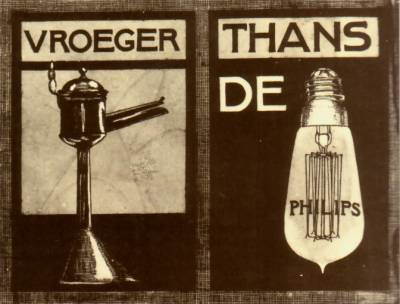
\includegraphics{./0_intro/img/1900-philips3.jpg}
\label{fig:incandescent_light_blub}
\caption{Early incandescent light bulb}
\end{figure}


From the first incandescent light bulb, the lighting industry has not had any big disruptive change to our perception of lighting till the last decade with the apparition of the LED lamps. Besides as many of us thing, it has been done a large effort to improve the efficiency of the light sources while keeping a the quality of the light as good as the incandescent light bulb. Being the florescent lamps one of the biggest contributions during the past century, beginning  to be commercialized around 1930. Later becoming a disruptive change in the lighting market with the introduction the low consumption lamps where Philips was one of the first player launching to the market the first screw-in fluorescent lamp. Although the prices of these lamps has been dropping to become commercially attractive for the costumers, their poorer color rendering factor and the longer setting time compared to the incandescent lamps prevented this lamps to be one-to-one replacement. Therefore the lighting industry has been keep without not too much attention till the introduction the LED based lamps.

\vspace{5mm} %5mm vertical space

\begin{figure}[!h]
\centering
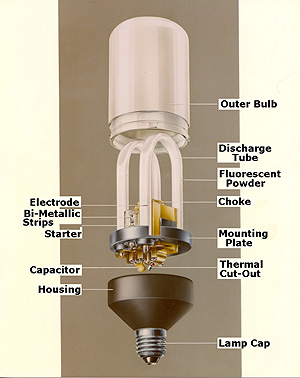
\includegraphics{./0_intro/img/phil1b.jpg}
\label{fig:philips_sl}
\caption{Components of the Philips SL compact fluorescent lamp. }
\end{figure}

The discovery of the high-efficiency blue LED ~\cite{94Nakamura} by Shuji Nakamura in 1994 enabled the quick development of the fist efficient withe LED. These early high power LEDs demonstrated that Solid State Lighting (SSL) devices  where a suitable technology for illumination. The relevance of Nakamura's work has been recognized last year being him awarded with the 2014 Nobel prize in physics. Looking farther we can also confirm the relevance of his invention since the apparition of the LED lamps, lighting is impacting again in our everyday life by changing our traditional concept of luminaries and lighting possibilities.

\begin{figure}[!h]
\centering
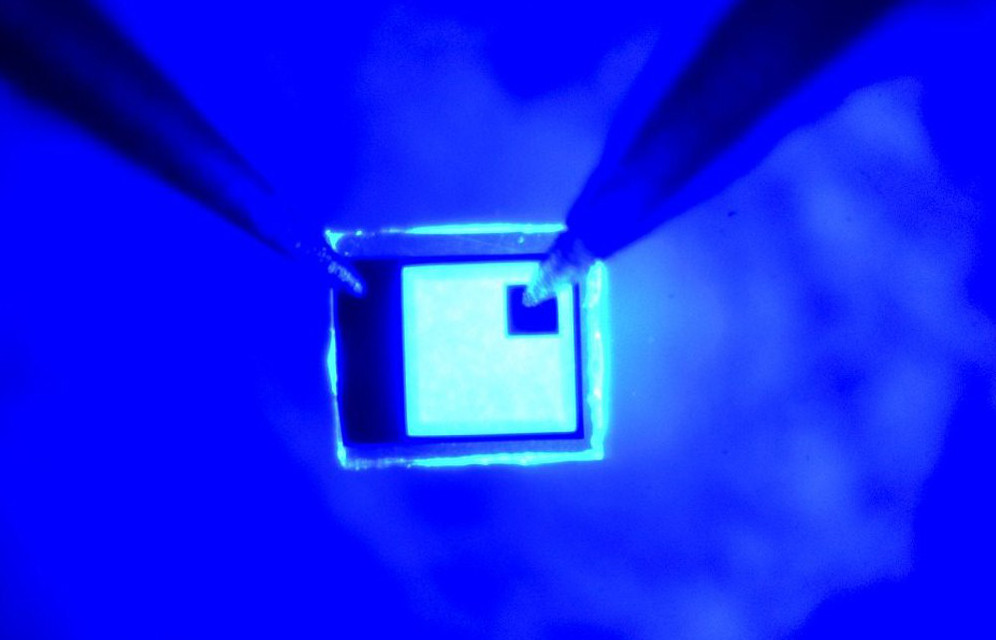
\includegraphics{./0_intro/img/10-7-14-nobel-prize-blue-led.jpg}
\label{fig:blue_LED}
\caption{Picture of a blue LED researched by Shuij Nakamura.}
\caption*{Source: \url{http://www.newsweek.com/how-blue-led-changed-world-and-won-nobel-prize-275977} }
\end{figure}

LED based lamps triggered  a frenetic rush in the lighting industry to bring that technology to the end consumers. Actually the large number of advantages of LED based lighting, or also known as Solid State Lighting (SSL), are so relevant that in the close future will replace any of the present lighting technology, that movement has been already named as the \emph{LEDification}. The principal advantages of SSL are:
\begin{description}
  \item [Efficiency] The light generation inside an LED is produced by the direct mechanism of hold-electron recombination, the supplied energy is a better use of the energy compared to the incandescent lamps. The power consumption can be up to an order of magnitude lower of an incandescent light.

  \item [Size] LEDs are tiny and flat devices, which can be considered as 2-D elements and do not need any vacuum chamber to work. They are much more flexible devices to assembly, and can easily replace the old glass made bulb design.

  \item [Color] LED light has a very narrow light spectrum, that can be used to produce directly colored light. Colored lights are becoming more popular in domestic homes becoming a piece of decoration or mood tweaking device.

  \item [Dynamics] Compared to any of the traditional sources of light LEDs have no dynamics, actually they have but it's very fast and not appreciable to the human eye. Therefore they do not have any setting time when turned on, which is not the case of CFL. The fast dynamics allows to modulate the light and transmit data without disturbing the human beings.

  \item [Lifetime] Solid State devices do not wear off, there fore they can be considered to have an infinite lifetime. In practice LEDs make use of organic phosphores, thus the light quality derates with the use, but the life expectancy of the LED is rated from 20.000 - 100.000 hours, multiplying 20 to 100 times longer that the classical light bulbs.
\end{description}

\vspace{5mm} %5mm vertical space

Bring the LED based lamps to the market is still a big challenge. Despite of the large number of advantages, the end consumers are still very reluctant to change generally due to the elevated costs of the new lamps, currently ranging between \$20 - \$40 for a 100W substitute compared to less than \$3 of an incandescent light. Also another issue that prevents consumers to change to the new technology is a poor light color consistency, light flickering and light dimming incompatibilities, that become really evident in low budget products.

\begin{figure}[!h]
\centering
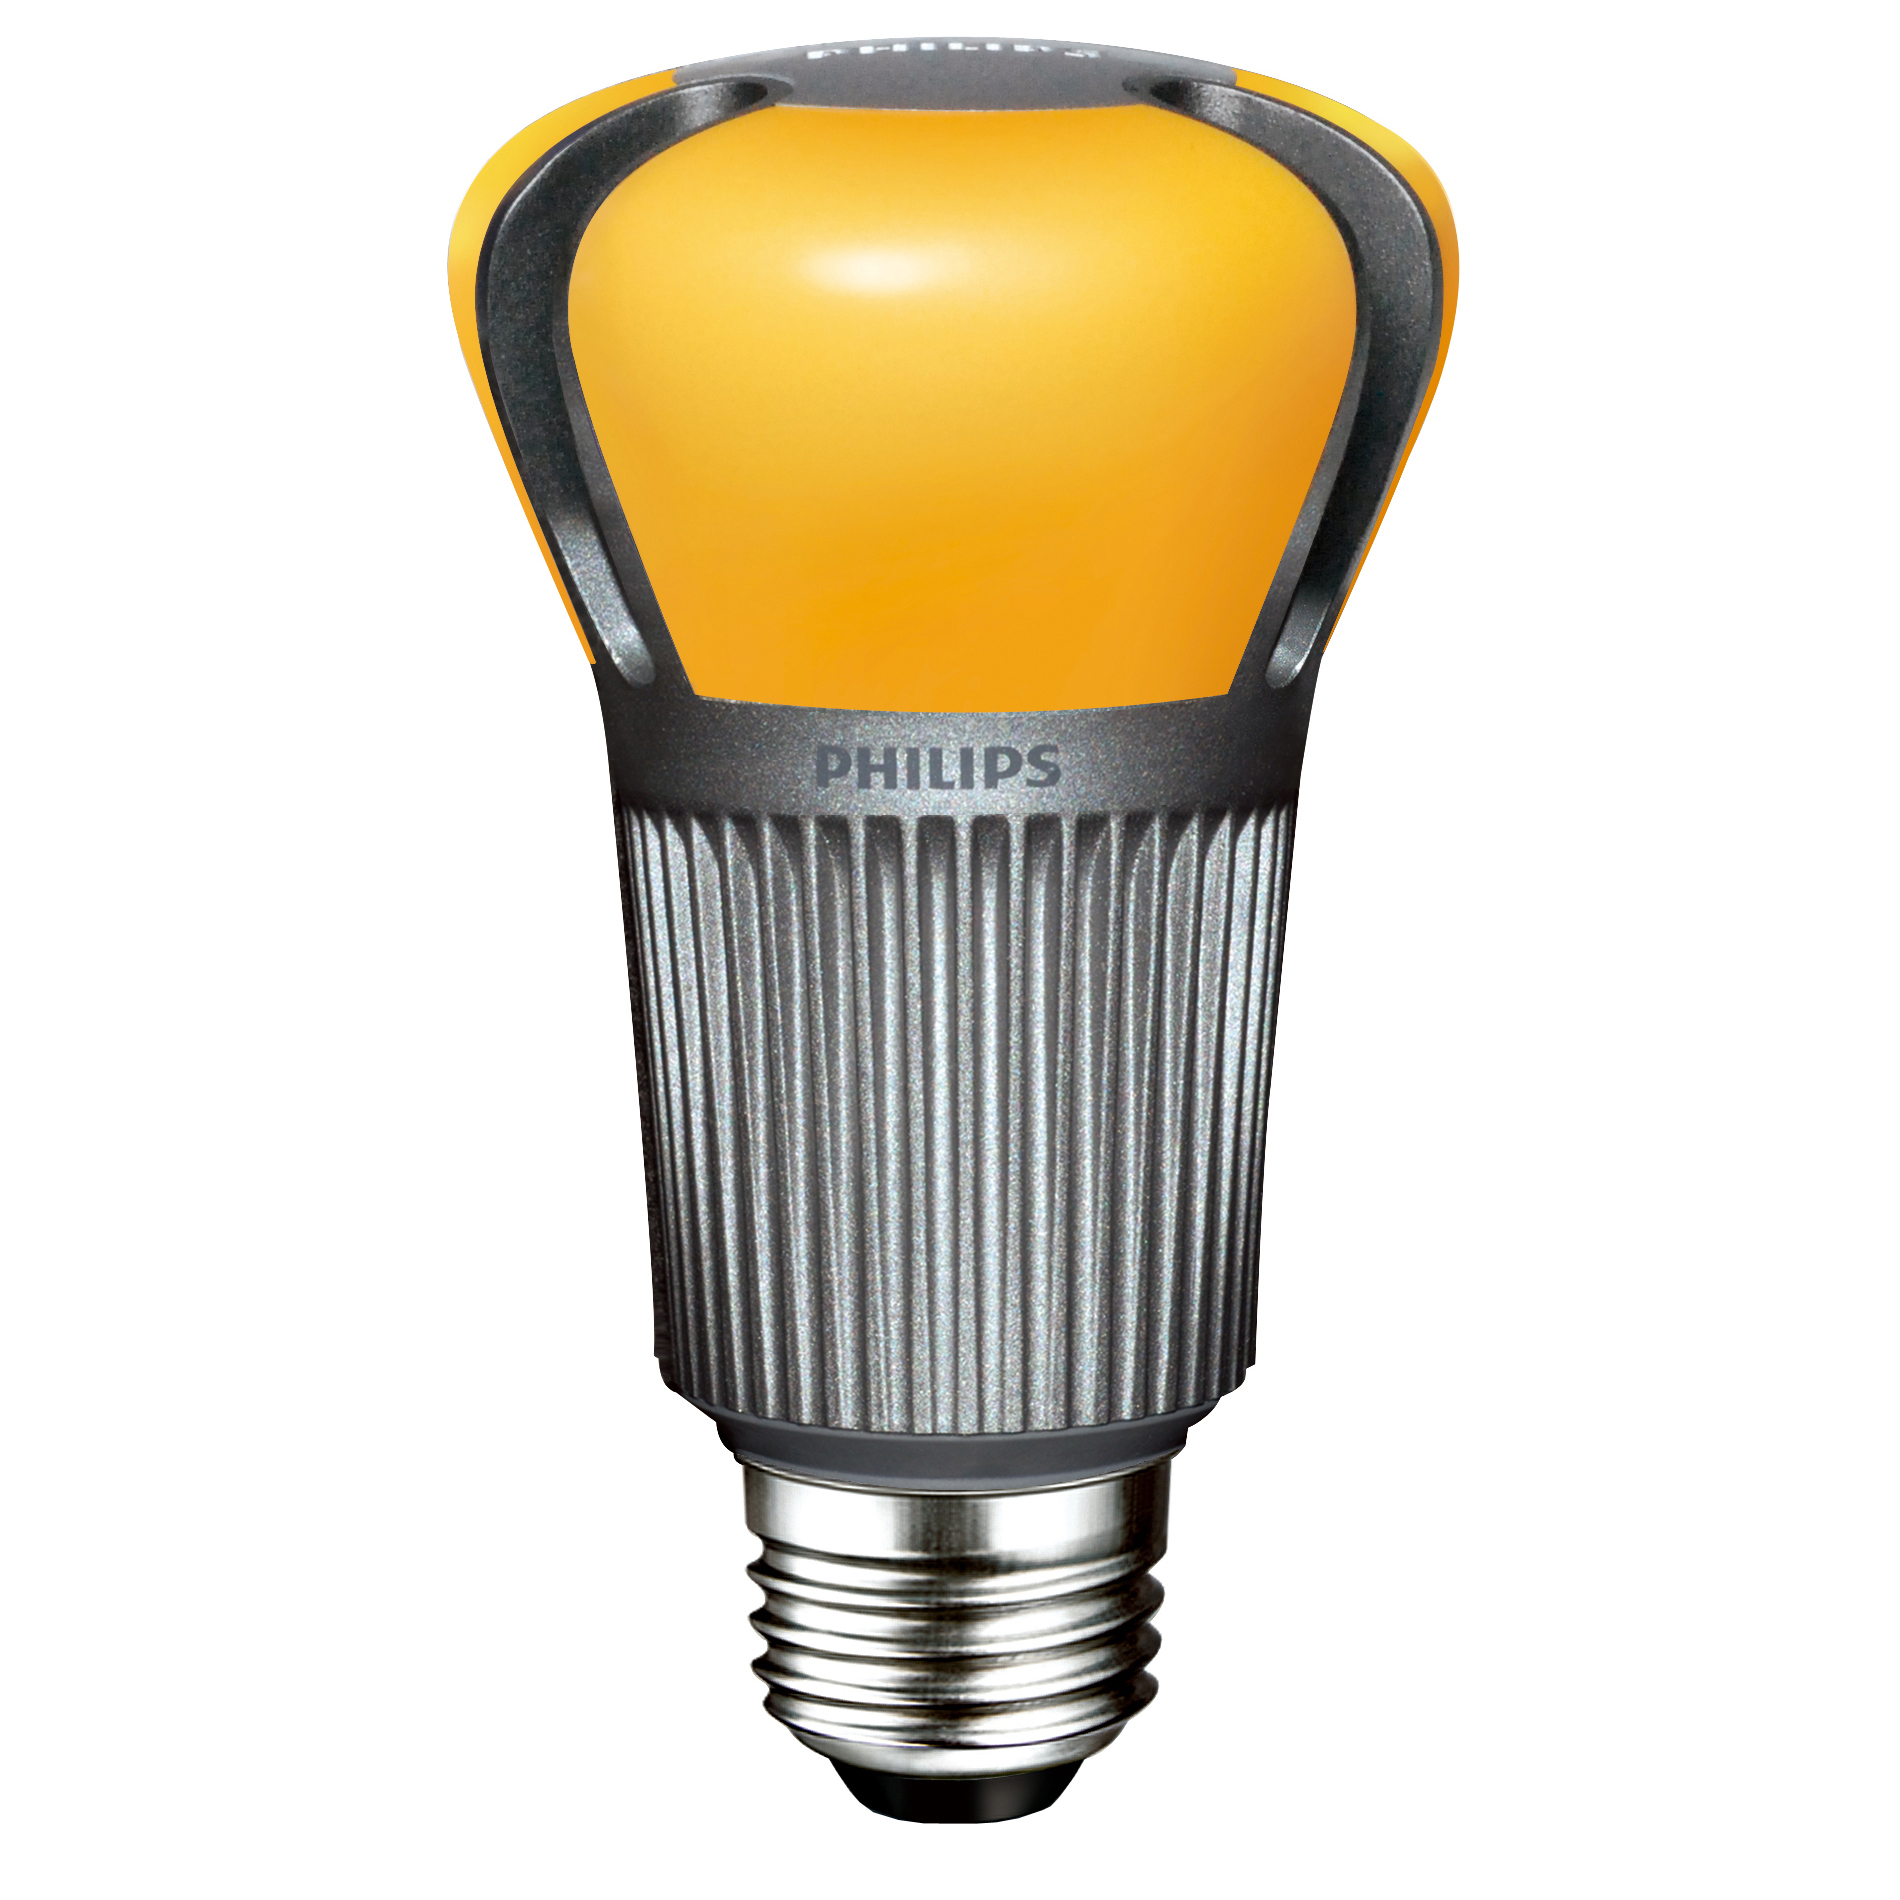
\includegraphics[width=4cm]{./0_intro/img/enduraled-12w.jpg}
\label{fig:l_prize}
\caption{900 lumens LED light bulb.}
\end{figure}

Two factors can be identified to make more favorable the adoption of the SSL as the preferred lighting solution by the consumers. In the one hand, reducing the end product price; and in the other hand, bringing more value to the traditional light sources. Actually LED light bulbs already bring more value compared to the old light bulbs being much more efficient, almost one order of magnitude lower in power consumption, and a longer lifetime, easily twenty times more operating hours. However these factors are not yet a valuable argument for the consumers. With the current trend of the \emph{internet-of-things} remote control, color tuning, light level dimming and integration to with future smart houses are probably some value propositions that people will need and SSL can easily provide. In a second level, I assume that the luminaries designs will change with a more favorable designs that take advantage of the low profiles of the LEDs.

 \begin{figure}[!h]
\centering
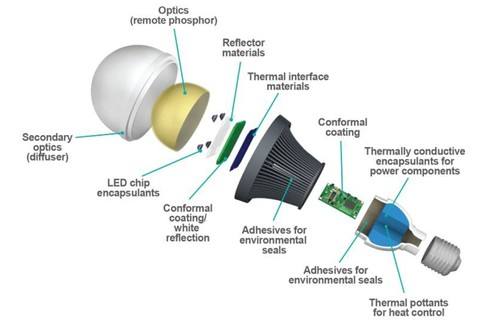
\includegraphics[width=8cm]{./0_intro/img/exploded_bulb_2.jpg}
\caption{Exploded vision of an LED light bulb.}
\label{fig:exploded_bulb}
\end{figure}

It is essential to describe the different elements in a LED light bulb in order to understand the challenges in its development and  design. A LED light bulb is composed by the six main elements described below and shown in  the Fig. ~\ref{fig:exploded_bulb}.

\begin{description}
  \item[LED] A two-lead semiconductor device that produced light when a current flows through it. The name comes from its acronym \emph{Light-Emitting Diode}. The light is produced by electroluminescence when an electron recombines with an electron-hole releasing energy in form of photons. The color of the light is determined by the energy band gap of the semiconductor.

   LED cost is very cheap and there is a broad assortment in colors, power and applications. The selection of the LED will determine: light color, voltage and current of the load, efficiency and necessary optics.

  \item[Optics] The optical device that helps to collimate, mix and distribute the light in the space in a desired way, normally uniformly for a determined projection area.

  \item[Driver] Electronic circuit placed between the input source and the load, the LEDs, that transforms the input electrical power to the requirements of the load. Since almost all the power distribution systems and storage devices are voltage sources and LEDs are current supplied loads, an LED driver is considered as current-to-voltage (V-I) power supply.

      The driver controls the current thought the load, hence the light output. Therefore it can be considered as the active part of the system where the control of the lamp relies. It is the most expensive and takes the largest volume of the lamp, and also one of the most or even the most important element in the entire system.

  \item[Heat sink] Mechanical element that acts as a passive heat exchanger and cools hot elements within the lamps system by dissipating the heat into the surrounding medium. The energy that is not converted to light becomes heat and must be extracted from the lamp, the main heat contributors elements are the LEDs and some components of the driver.

      The costs of the heat sink is also a relevant part in the total cost of the lamp.

  \item[Body assembly] Mechanical element that hold all the different subsystems in one single device. In many cases the heat sink does this functionality.

  \item[Connector] Mechanical element that provides connection with the energy source. The most popular one is the Edison connector present in all screw-in lamps. There are many other popular ones such as GU10, MR16, MR11 coming from the halogen multifaceted reflector bulbs or the 2-pin connector of the fluorescent tubes.

      In many cases, the standardized connectors suppose a restriction for the mechanical design of the lamp. Their old-fashioned design is not optimal for the new lamps.


\end{description}

\vspace{5mm} %5mm vertical space

The chart shown in Fig.\ref{fig:cost_breakdown} makes evident that the driver is the most expensive part of the system. As it was previously mentioned, the driver is the key component in the functionality of the LED lamp, since it controls the light output and at the same time determines the efficiency of the system. Therefore, the LED driver has become on of the hot topics of research within the power electronics field. Besides the necessity of fulfilling the operational requirements, such as high efficacy an proper power quality, two main issues have trigger research around the driver circuit: The costs and the volume.
\begin{figure}[!h]
\centering
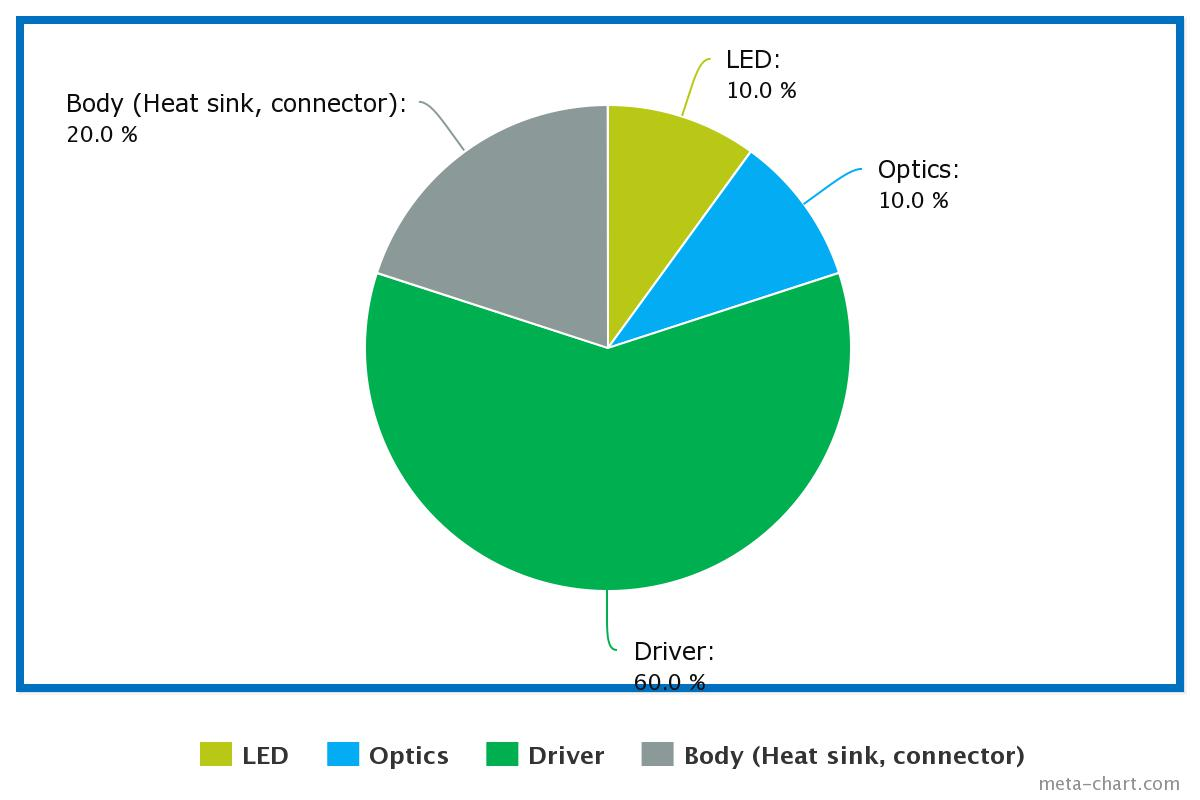
\includegraphics[width=8cm]{./0_intro/img/piechar_costs.jpeg}
\caption{LED lamp cost breakdown by subsystems.}
\label{fig:cost_breakdown}
\end{figure}

\vspace{5mm} %5mm vertical space

The cost of the driver is one of the biggest problems that SSL industry has been dealing after the power LEDs become a commodity components. Actually, this piece of electronics was not present in the incandescent light bulbs, thus its elevated cost arose as an inconvenient and difficult to justify in the new light bulbs. Philips Research has devoted a large effort in that field, being indeed the main focus of research regarding the LED drivers.


Reducing the costs of the lamps has been the strategy taken for the first wave in the \emph{LEDification} process where retrofitting\footnote{Adding the new LED technology to the older light bulb systems. In that way the end user can directly replace an incandescent lamp or a florescent tub by an LED one without needing to make any change in the current installation.} the old lamps is chosen as the way to target the end costumer. In on the one hand, fruitful results came form that research with new innovative solutions at very low costs that could be packed in almost all the light bulb shapes currently commercially available. But in the other hand, these new drivers had the incontinent of using very old components that at the same time restricted reduction of the circuit volume and made more complex the addition of extra control functionalities while keeping the initial low costs.

\begin{figure}[!h]
\centering
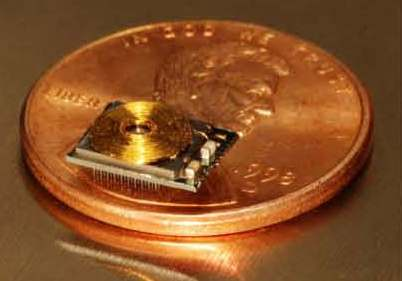
\includegraphics[width=8cm]{./0_intro/img/FSolzbacher01.jpg}
\caption{Power System in a Package die. The circuit implements a buck converter.}
\label{fig:psoc_example}
\end{figure}

\vspace{5mm} %5mm vertical space

The second line of research has focus on reducing the volume of the driver circuit. That research topic arose when comparing the the volume of the LEDs and the driver, it is evidenced a mismatch between the two volume of the components, becoming in many cases the driver circuit the dominant element of the entire lamp. Such mechanical constrain supposes an obstacle to take the full advantage of the low form-facto of the LED in the future luminaries, where LED will not be assembled using the old fashioned cases. Therefore, that research has a much longer term vision for targeting the second of third generation of lights in the \emph{LEDification} process.

The drive to reduce the volume of the drivers led to focus the research from the perspective of the integrated power supplies, where the power converter can be partially or fully integrated in a single package. There are two approaches of integrated power converters: \emph{Power System on Chip} (PSoC) or  \emph{Power System in Package} (PSiP). The first integrate all required power components, active and passive, in a single die. The second assemble all the components within the same package, keeping the appearance of an unique \emph{Integrated Circuit} (IC), see Fig.\ref{fig:psoc_example}. The advantages of having an integrated power management unit align with the necessities of the LED drivers, therefore trend of the drivers will be going towards having \emph{Power LED Drivers in Package} (PLDiP).

Besides the size reduction that an integrated driver would suppose, an integrated approach would also bring other benefits in terms of control and connectivity. Since such a solution would require a the design of a dedicated \emph{application-specific integrated circuit} (ASIC), the power management unit and driver control unit can be integrated together, providing the necessary intelligence for light control and the connectivity optimized for the requirements of the coming connected lighting industry. The \emph{Philips} \emph{HUE} lamp is a clear example of the requirements of the so called \emph{smart drivers}. That lamp provides a full light color gamut color control through a mobile and web application or through a remote control. The internal driver has four light channels red, green, orange and additional amber and at the same time provides wireless connectivity through ZigBee, being the electronic board populated with discrete power drivers and few micro-controller units. A solution that integrates all the functions in a single IC, or few ICs (one per channel), will definitely reduce packaging and assembling costs and still providing the same functionalities. And at the same time, the expected market size for LED lighting to justify a dedicated ASIC design for the light bulbs and indeed has been the motivation of this thesis. Therefore goal of this work was to explore and identify new architectures that are suitable for integration and at the same time can perform as an efficient LED driver.


\section{Why a LED needs a driver?}

As shown in Fig. \ref{fig:led_I-V} a LED has a very abrupt V-I curve. For voltages below the \emph{forward voltage}, $V_{f}$, there is no current flow and the LED behaves as an open circuit. For voltages above $V_{f}$ the curve becomes very steep and the current increases dramatically with respect to the voltages, thus the LED behaves as short circuit. The driver bias the LED to a specific point, $P$ in Fig. \ref{fig:led_I-V}, providing the desired output light. The colour and flux (light intensity) will vary depending of the bias point.  Since the majority of  available  energy sources are  voltage sources, and LED requires a circuit that limits the current that flows through it, that circuit is the LED driver.

\begin{figure}[!h]
\centering
\begin{tikzpicture}[domain=0:5]
    \draw [->] (0,0) -- (4.5,0) node[anchor=west]{$V$};
    \draw [->] (0,0) -- (0,4.5) node[anchor=east]{$I$};

    %Mark Vth
    \draw (2,2pt) -- (2,-5pt) node[anchor=north] {$V_{f}$};

    %Draw ideal plot
    \draw[thick] (0,0) -- (2,0) -- (4,4);

    %Draw bias points
    \draw[dashed] (3,2) -- (3,-0);
    \draw (3,2pt) -- (3,-5pt) node[anchor=north]  {$V_{bias}$};

    \draw[dashed] (3,2) -- (-0,2);
    \draw (2pt,2) -- (-5pt,2) node[anchor=east]  {$I_{bias}$};
    \filldraw (3,2) circle(2pt) node[anchor=west] {$P$};

  

\end{tikzpicture}
\caption {}
\label{fig:led_I-V}
\end{figure}

At the first glance, keeping a constant bias current, $I_bias$, through the LED does not seems to be challenging. However LED V-I characteristic is not static, in practice LEDs has different source of deviations and drivers have to deal with them in order to keep delivering the desired light output. First, $V_f$ has a negative dependence with the temperature, drooping its values as the PN junction temperature increases. Second, the LED has an aging factor derating its light output over time, which has to be adjusted by changing the bias point. And last but not least, during production LEDs will vary in colour, flux and forward voltage; even for products from the same batch. The manufacturer reduced the dispersion between devices by binning \footnote{Quality control performed at LED production line, where each LED is individual tested and sorted in groups (bins) that have the same electrical and lighting characteristics.}, but still after binning it can be deviations from up to $10\%$ in $V_f$ for the same part number.

Up to date, there are three families of LED drivers:

\begin{description}
  \item[Linear Drivers] place a shunt element between the source and the LED. The shunt element limits the current in the LED providing the necessary voltage droop between the source and the load. The excess of voltage between the source and the load is dissipated in the shunt element, literally burned in form of heat; therefore this drivers become very inefficient if the LED voltage is not close to the source. Moreover this drivers can only provide step-down conversion, thus they cannot work when the load voltage is higher than the input supply.

      \begin{figure}[!h]
        \centering
        \ctikzset { bipoles/length=1cm}
        \begin{circuitikz} [american,scale=0.65]
        \draw
        (5,0) to[short]
        (0,0) to[V = $v_{src}$]
        (0,3) to[generic=${Shunt}$]
        (5,3);
        \draw
        (5,0) to[leD*,mirror,v>=$v_{o}$,i<=$i_o$] (5,3); 
        
        \begin{scope}[xshift = 8cm, yshift=0cm]
            \draw[->] (0,0) -- (4,0) node[anchor=north] {$  m $};
            \draw[->] (0,0) -- (0,3) node[anchor=west] {$\eta $};
            
            %Ticks X 
            \draw (3,2pt) -- (3,-5pt) node[anchor=north] {$1$};
            \draw (1.5,2pt) -- (1.5,-5pt) node[anchor=north] {$0.7$};
            
            %Ticks Y
            \draw (2pt,2.5) -- (-5pt,2.5) node[anchor=east] {$100\%$};
            \draw (2pt,1.5) -- (-5pt,1.5) node[anchor=east] {$70\%$};
            
            %Markers
            \draw[dotted] (3,2.5) -- (3,0);
            \draw[dotted] (3,2.5) -- (0,2.5);
            \draw[dotted] (1.5,1.5) -- (1.5,0);
            \draw[dotted] (1.5,1.5) -- (0,1.5);
            
            
            \draw[thick] (3,2.5) -- (0,0.5);
            
            
            
        \end{scope}
        
        \end{circuitikz}
        \label{fig:linear_drv}
        \caption{Linear LED driver schematic} 
       \end{figure}
      
   The circuit of the Fig. \ref{fig:linear_drv} shows schematic of a linear driver, the shunt element can be implemented with just a resister of with an active device, the second enables regulation for variations in the source and in the load. Both cases linear drivers are very simple to implement, with very low costs and taking almost no volume, being indeed the perfect solution for integration.
   
   The plotted graph presents the variation of the driver efficiency with respect to the conversion ration $m$. $m$  is the ratio between the input voltage, $v_{src}$,  and the output voltage,$v_o$, being defined as
   \begin{equation}
        m = \frac{v_o}{v_{src}}.
   \end{equation}
   
   The efficiency of the driver is the ratio between the input power and the output power
   \begin{equation}
        \eta = \frac{P_o}{P_i} = \frac{v_o i_o}{v_{src} i_o} = \frac{v_o}{v_{src}},
   \end{equation}
   thus we can see that for this case the efficiency is indeed the conversion ratio
   \begin{equation}
        \eta = m,
   \end{equation} 
   owing to the fact that LED drivers have to be efficient, saying that at worst case 80\% efficiency can be accepted, such drivers could only be suitable where the ration between input voltage and load voltage is 0.8.  
   
   Despite the fact that linear drivers are cheap and easy to integrate, their poor efficiencies and limitations in power conversion palace them in a unfavorable position as a realistic sortition for an integrated solution.  
   
   


  \item[Inductor Based Converters] are \emph{Switched Mode Power Supplies} (SMPS) 
  \item[Switched Capacitors] dfa
\end{description}


\chapter{Different types of Drivers}




%\section{DC-DC Drivers}
%\section{AC-DC Drivers}

\chapter{Switched capacitors for LED drivers}

There are two families within the integrated power supplies, inductor based converters and switched capacitors based converters. Inductor based converters make use of magnetic passive components as energy storage for the power conversion, being the most common converters used for LED drivers for to lighting. These converters easily achieve very large efficiencies while providing excellent current regulation output. However the magnetic devices restricts the integration of these converters. Switched Capacitor Converters (SCC) provide energy conversion using capacitors as a energy storage



%\label{ch:h_scc}
%%%%\bibliographystyle{numerical}
\chapter{Introduction}

The challenges in powering LED loads are so relevant that have an impact in functionalities and design of the future \emph{Solid-State-Lighting} (SSL) products. So much, that the user adoption of such a beneficial technology by is far slower than comparable disruptive technologies~\cite{11Voger}. In a part, that could be attributed due to the difficulties in achieving the high miniaturization and performance necessary in the LED drivers, at low cost, in order to outcompete the cheaper old technologies.

From the power management standpoint power a LED load is a trivial task, however the different requirements of SSL products make the design of them a complex task. Initially the main driving forces in the driver designs where: manufacturing cost, power quality, light quality. Reducing manufacturing costs can enable to decrease the lamp prices to the entry point for the consumers. The drivers have to fulfill with the legislation in terms of power quality not exceeded the minimum \emph{Power Factor} (PF) and \emph{Total Harmonic Distortion} (THD). From the consumer point of view the light quality is measured in terms of: flickering, color consistency and \emph{Color Rendering Index} (CRI), being the flickering a parameter related to the driver design. Flickering must be kept  under certain limits to do cause health concerns~\cite{10Wilkins}.
Recently two other factors are becoming more relevant in the driver: miniaturization and  controllability. The volume of the drivers is currently, in many cases, limited by the old lamp shapes in order to provide retrofit solutions. There are solutions for all incandescent lamps, however there are still challenged for small halogen cases. Anyway the miniaturization requirements of the lamps have been relaxed by redefining the shape and look of the old lamps, the new design take large part of the lamp volume for the heat sink body, what allows a large volume for the driver. Further reduction of the driver will enable higher freedom in the lamp design. The future connected lamps~\cite{14Harbers} will require control and connectivity, what challenges the driver to provide multiple color channels, current control and power management for added intelligent circuitry such as MCUs and sensors.

The high and diverse level of requirements for the LED drivers has made the design process a complex task, further than just a pure power management problem. The initial driving forces in driver design, cost, power and light quality, found effective solutions  based on discrete components.  The new driving forces where miniaturization, controllability and connectivity brings to research in the context of \emph{Power Systems on-Chip/in-Package}(PSoC/PSiP), where miniaturization and integration of functionalities can be easily achieved. This chapter starts with an analysis of the LED characteristics to understand why is a driver necessary. Subsequently, the three different driver technologies are studied: Linear, switched inductor converters and switched capacitor converters. An state-of-the-art for each technology will be provided in order to construct a rational of the technology toward miniaturization. Switched capacitor converters will be thoroughly studied, since constitute the central conversion technology selected for this dissertation.


\section{The LED load}
\label{sc:LED_load}
The LED is just a special diode that emits light as the acronym stands for \emph{Light Emitting Diode}. It is well known that a diode has a very \emph{voltage-current} ($v-i$) curve as shown in Figure~\ref{fig:led_I-V}. For voltages below the \emph{forward voltage}, $v_{f}$, there is practically no current flow and the LED behaves as an open circuit. The same characteristic applies  when reversed bias until the breakdown voltage, $v_{break}$, is reached. For voltages above $v_{f}$ the curve becomes very steep and the current increases dramatically with respect to the voltage, thus the LED behaves as a short circuit. The similar behaviour happens when the LED is reverse biased and the voltage is above $v_{break}$, however in this case there is no light generation. The LED has to be supplied at an specific point $P$ in order to provide a desired light output as shown in Figure~\ref{fig:led_I-V}, depending on the bias current light colour and intensity will vary. Due to the steepness in the $v-i$ curve, the practical way to bias a LED is supplying them with a \emph{dc}-current. Since the common used energy sources are voltage supplies, it is necessary to select a circuit that converts the input energy from the voltage source to a constant current.

\begin{figure}[!h]
\centering
\begin{circuitikz}[american voltages]

    \draw (0,2.5) to[leD*,v=$v$,i=$i$,*-*] (3
    ,2.5) ;

\begin{scope}[xshift=4cm, domain=0:6]
    \draw [->] (0,0) -- (5.5,0) node[anchor=west]{$v$};
    \draw [->] (0,0) -- (0,5.5) node[anchor=east]{$i$};

    %Mark Vth
    \draw (2,2pt) -- (2,-5pt) node[anchor=north] {$v_{f}$};

    %Mark Vthmin and Vt_max
    \def\dvf{0.25}
    \def\dvftop{0.45}

    \draw (1.5,2pt) -- (1.5,-5pt) node[anchor=north] {};
    \draw (2.5,2pt) -- (2.5,-5pt) node[anchor=north] {};
    \draw[dotted] (1.5,0) -- (1.5,\dvftop);
    \draw[dotted] (2.5,0) -- (2.5,\dvftop);
    %Mark Delta Vf
    \draw[pil,>-< ,dotted] (1.25,\dvf) -- (2.75,\dvf);
    \draw (1,\dvf) -- (1.5,\dvf) node[anchor=south east] {$\Delta v_f$};


    %Draw ideal plot
    \draw[thick] (0,0) -- (2,0) -- (4.5,5);

    %Draw lower limit
    \draw[dashed] (0,0) -- (1.5,0) -- (4,5);
    %Draw higher limit
    \draw[dashed] (0,0) -- (2.5,0) -- (5,5);

    %Draw bias point projection
    \draw[dotted] (4,4) -- (4,-0);
    \draw (4,2pt) -- (4,-5pt) node[anchor=north]  {$v_{bias}$};

    \draw[dotted] (4,4) -- (-0,4);
    \draw (2pt,4) -- (-5pt,4) node[anchor=east]  {$i_{bias}$};

    %Draw bias point
    \filldraw (4,4) circle(2pt) node[anchor=south west] {$P$};

    %Draw bias point variations
    \draw (4.5,4)  node[anchor=south west] {};
    \draw (3.5,4)  node[anchor=south west] {};

    %\draw[loosely dotted] (4.5,4) -- (4.5,-0);
    %\draw[loosely dotted] (3.5,4) -- (3.5,-0);
    \draw (4,2pt) -- (4,-5pt) node[anchor=north]  {$v_{bias}$};
    %Mark Vthmin and Vt_max
    \def\bpmi{4.5}
    \def\bpMa{3.5}
    %\draw (1.5,2pt) -- (1.5,-5pt) node[anchor=north] {};
    %\draw (2.5,2pt) -- (2.5,-5pt) node[anchor=north] {};
    %\draw[dotted] (1.5,0) -- (1.5,\dvftop);
    %\draw[dotted] (2.5,0) -- (2.5,\dvftop);
    %Mark Delta Vf
    %\draw[pil,>-< ,dotted] (3.25,\dvf) -- (4.75,\dvf);
    %\draw (4.5,\dvf) -- (5,\dvf) node[anchor=south west] {$\Delta V_{bias}$};

    %Mark Vthmin and Vt_max
    \def\dvf{4}
    %\draw (1.5,2pt) -- (1.5,-5pt) node[anchor=north] {};
    %\draw (2.5,2pt) -- (2.5,-5pt) node[anchor=north] {};
    %\draw[dotted] (1.5,0) -- (1.5,\dvftop);
    %\draw[dotted] (2.5,0) -- (2.5,\dvftop);
    %Mark Delta Vf
    \draw[pil,>-< ,dotted] (3.25,\dvf) -- (4.75,\dvf);
    \draw (4.5,\dvf) -- (5,\dvf) node[anchor=south west] {$\Delta v_{bias}$};


\end{scope}
\end{circuitikz}
\caption{Idealized LED voltage-current characteristic, with the \emph{forward voltage} $v_f$  identified and a projection of the \emph{bias point} P }
\label{fig:led_I-V}
\end{figure}

At first glance, keeping a constant bias current, $i_{bias}$, through the LED does not seems to be challenging, however the LED's electrical characteristics are not static and have some tolerances. On the one hand, a LED has different sources of deviations that the driver circuit has to deal with them in order to keep them delivering the desired light output. First, $v_f$ has a negative dependence with the temperature, drooping its values as the \emph{pn}-junction temperature increases. Second, the LED has an aging factor which derates the light output over time, and which has to be adjusted by changing the bias point. And last, during production LEDs will vary in colour, flux, and forward voltage; even for products from the same batch. The manufacturers have reduced the tolerances between devices by binning \footnote{Quality control performed at LED production line, where each LED is individual tested and sorted in groups (bins) that have the same electrical and lighting characteristics.}, but after binning, the parts suffer deviations, \emph{e.g.} up to $10\%$ in $v_f$. Figure ~\ref{fig:led_I-V} shows graphically how deviations in $v_f$ produce a displacement in the $v-i$ characteristic,  which require to modify the $v_{bias}$ within a certain range $\Delta v_{bias}$ in order to keep $i_{bias}$ constant. On the other hand, the voltage provided by the energy supply has some tolerances. Depending on the nature of the energy supply, \emph{ac} or \emph{dc}, the driver has to provide line regulation, filter high frequency perturbations and accept the voltage tolerances of the source, without affecting the light output. In general, LEDs lamps have to provide a certain desired light output range despite variations in the LED characteristics or the voltage supply, and therefore that control function is what adds complexity to the driver circuit. The three families of LED drivers will be presented in the subsequent sections.

\section{Linear Regulators}
Linear drivers place a shunt element between the source and the load(\emph{i.e} the LED). The shunt element limits the LED current providing the necessary voltage droop between the source and the load. The excess of voltage between the source and the load is dissipated in the series element, literally burned in form of heat; therefore these drivers become very inefficient if the LED voltage is not close to the source. Other limitation is that linear drivers only provide step-down conversion, thus they cannot work when the voltage at the load is higher than the input supply.

\begin{figure}[!h]
\centering
\ctikzset { bipoles/length=1cm}
\begin{subfigure}[t]{.45\textwidth}
    \centering
    \begin{circuitikz} [american voltages,scale=0.65]
    \draw
        (0,0) to[V = $v_{src}$]
        (0,3) to[generic=$r_series$,i=$i_o$]
        (5,3) to[leD*,v=$v_{o}$]
        (5,0) -- (0,0);
    \end{circuitikz}
    \caption{}
    \label{fig:linear_ckt}
\end{subfigure}
\begin{subfigure}[t]{.45\textwidth}
    \begin{circuitikz} [scale=0.65]
    \begin{scope}%[xshift = 8cm, yshift=0cm]
        \draw[->] (0,0) -- (4,0) node[anchor=south] {$  m $};
        \draw[->] (0,0) -- (0,3.2) node[anchor=east] {$\eta $};

        %Ticks X
        \draw (3,-5pt) -- (3,2pt)  node[anchor=south west] {$1$};
        \draw (1.5,-5pt) -- (1.5,2pt)   node[anchor=south west] {$0.7$};

        %Ticks Y
        \draw (2pt,2.5) -- (-5pt,2.5) node[anchor=east] {$100\%$};
        \draw (2pt,1.5) -- (-5pt,1.5) node[anchor=east] {$70\%$};

        %Markers
        \draw[dotted] (3,2.5) -- (3,0);
        \draw[dotted] (3,2.5) -- (0,2.5);
        \draw[dotted] (1.5,1.5) -- (1.5,0);
        \draw[dotted] (1.5,1.5) -- (0,1.5);


        \draw[thick] (3,2.5) -- (0,0.5);
    \end{scope}
    \end{circuitikz}
    \caption{}
\label{fig:linear_chr}
\end{subfigure}
\caption{Linear driver, \emph{left}- schematic; \emph{righ}- conversion ratio vs. efficiency characteristics}
\label{fig:linear_drv}
\end{figure}

The circuit of the Figure~\ref{fig:linear_ckt} shows the schematic of a linear driver. The shunt element can be implemented with just a resistor of with an active device. The first will impose a current depending on the input source and the load conditions; the second will provide regulation of the bias point for variations in the source and in the load. Linear drivers are very simple to implement, with very low costs and taking almost no volume, being indeed the perfect solution for integration since they do not make use energy storage components for power processing.

The plotted graph in Figure~\ref{fig:linear_chr} presents the variation of the driver efficiency with respect to the conversion ration $m$. Here $m$  is the ratio between the input voltage, $v_{src}$,  and the output voltage,$v_o$, being defined as
   \begin{equation}
        m = \frac{v_o}{v_{src}}.
   \end{equation}

The efficiency of the driver is the ratio between the input power and the output power
   \begin{equation}
        \eta = \frac{P_o}{P_i} = \frac{v_o i_o}{v_{src} i_o} = \frac{v_o}{v_{src}},
   \end{equation}

hence for this case the efficiency is indeed equal to the conversion ratio
   \begin{equation}
        \eta = m.
   \end{equation}
Owing to the fact that LED drivers have to be efficient, and assuming that a worst case 80\% efficiency can be accepted, linear drivers could only be suitable where the ration between input voltage and load voltage is higher than 0.8.


\section{Inductor Based Converters}

\emph{Inductor Based Converters} (IBCs) are \emph{Switched Mode Power Supplies} (SMPS) \footnote{Electronic power supply that provides efficient electric power conversion by commuting between different circuit configurations (modes).}  that employ magnetic passive elements (i.e. inductors and transformers) to store energy and provide efficient electrical power conversion. Since IBCs are very efficient with respect to voltage-to-current conversion, they are ideal as LED drivers.

The inductor is the main element in these converters and it allows voltage conversion by storing energy in form of magnetic field. In the case of the converter of the figure~\ref{fig:induct_ckt} the inductor is charged during

These converters can provide step-up and step-down conversion for large dynamic ranges while keeping the efficiency very high. On top of their power conversion capabilities, such converters can also provide galvanic isolation, which in many applications is compulsory in order to guarantee the safety of the users against electrical hazards. Such characteristics suggest these drivers as the preferred solution for the LED industry. Figure~\ref{fig:induct_ckt} shows one of the most popular implementations for LED drivers: The \emph{buck} converter.  Figure~\ref{fig:induc_chr} presents the regulation characteristic of a generic  inductor based converter. As shown, the theoretical efficiency of these converters is 100\% for all the conversion ratio range. In practice, due to parasitics in switches and inductors, the efficiency drops to a certain value with small fluctuations with respect to the conversion range.

\begin{figure}[!h]
\centering
\ctikzset { bipoles/length=1cm}
\begin{subfigure}[t]{.45\textwidth}
    %\centering
    \raggedright
    \begin{circuitikz} [american voltages,scale=0.65]
    \draw
        (6.5,0) to[short]
        (0,0) to[V = $v_{src}$]
        (0,3) to[switch]
        (3,3) to[inductor=${L}$,i=$i_o$]
        (6.5,3);

    \draw (2.5,3) to[switch] (2.5,0);

    \draw (6.5,3) to[leD*,v=$v_{o}$] (6.5,0);

    \end{circuitikz}
    \caption{}
    \label{fig:induct_ckt}
\end{subfigure}
\hfill
\begin{subfigure}[t]{.45\textwidth}
    %\centering
    \raggedleft
    \begin{circuitikz} [scale=0.65]
    \begin{scope}%[xshift = 8cm, yshift=0cm]
        \draw[->] (0,0) -- (4,0) node[anchor=south] {$  m $};
        \draw[->] (0,0) -- (0,3.2) node[anchor=east] {$\eta $};

        %Ticks X
        %\draw (3,2pt) -- (3,-5pt) node[anchor=north] {$1$};
        %\draw (1.5,2pt) -- (1.5,-5pt) node[anchor=north] {$0.7$};

        %Ticks Y
        \draw (2pt,2.5) -- (-5pt,2.5) node[anchor=east] {$100\%$};
        \draw (2pt,1.5) -- (-5pt,1.5) node[anchor=east] {$90\%$};

        %Markers
        % \draw[dotted] (3,2.5) -- (3,0);
        \draw[dotted] (3,2.5) -- (0,2.5);
        %\draw[dotted] (1.5,1.5) -- (1.5,0);
        \draw[dotted] (1.5,1.5) -- (0,1.5);


        \draw[thick] (0.5,2.5) -- (3,2.5) node[anchor=south] {$Theoretical$};
        \draw[thick,dashed] (0.5,1.20) parabola[bend at end] (3,1.7) node[anchor=north] {$Real$};
    \end{scope}
    \end{circuitikz}
    \caption{}
\label{fig:induc_chr}
\end{subfigure}
\caption{Inductor based converter, \emph{left} - buck converter schematic; \emph{right} - conversion ration \emph{vs.} efficiency curve comparing the \emph{theoretical} and a \emph{practical} limit. }
\label{fig:inductive_smps}
\end{figure}

One of the disadvantages of these converters is the magnetic components, and the volume related to them. In practice, inductors dominate the entire volume of the LED drivers as shown in Figure~\ref{fig:smps_driver}. Integrated implementations of these converters suffer the challenges of using integrated magnetic components. The present \emph{very-large integration scale} (VLSI) technologies do not yet offer power inductors in the commercial implementations, and other integrated inductors are not yet mature enough for non-research products.

Yet another disadvantage for integration is the voltage stress in the switches of the converter. Switches in inductive converters have to withstand the full operational voltage, which depending on the application range, is from tens to a few hundreds of volts. Using high voltage devices has three main drawbacks: First, the losses in the devices scale quadratically with the voltage  stress. Second, bad switching performances, because high voltage devices are less efficient and slower switching. Third, the standard VLSI technologies do not offer these \emph{high voltage} (HV) devices and the VLSI technologies that offer them are less performant and more expensive than the dedicated discrete technologies.

\begin{figure}[!h]
\centering
\begin{tikzpicture}
\node[anchor=south west,inner sep=0] (image) at (0,0) {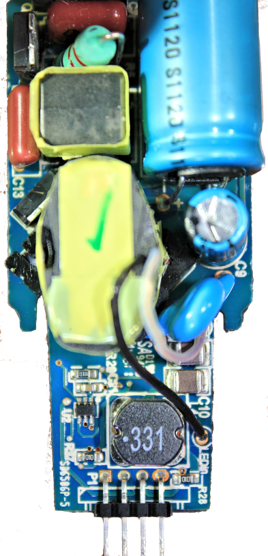
\includegraphics[height=5cm,angle=90]{./0_intro/img/LED_driver.png}};
\begin{scope}[x={(image.south east)},y={(image.north west)}]
%\draw [<-,thick] (0.75,0.5) -- (0.855,0.7)  node [anchor=south west] {Power Magnet};
\draw[black,ultra thick,rounded corners] (0.70,0.3805) rectangle (0.855,0.7);
\draw[black,ultra thick,rounded corners] (0.11,0.1) rectangle (0.28,0.50);
\draw[black,ultra thick,rounded corners] (0.28,0.1) rectangle (0.63,0.62);
\end{scope}
\end{tikzpicture}
\caption{Magnetic components marked with a black square in a mains connected LED driver. These components dominate the volume of the converter.}
\label{fig:smps_driver}
\end{figure}


\section{Capacitor Based Converters }
Switched Capacitor Converters (SCCs) are SMPS composed only of switches and capacitors. SCC were initially used for voltage multiplication~\cite{30Cockcroft,44Waidelich,76Dickson} and more recently in applications that need voltage regulation as well~\cite{Ng:EECS-2011-94}. Compared to inductor based converters, the absence of magnetic elements places them in a good position for high density power systems and integrated solutions, such as Power-System-in-Package (PSiP) or Power-System-on-Chip (PSoC).

SCCs have a fixed ratio of conversion between the input and the output determined by the topology. The output voltage of the converter under no load conditions is defined as the \emph{target voltage} $v_t$. The converter performs at high efficiency when the load is supplied close to the \emph{target voltage}. Similar to the linear drivers, if the output voltage goes below the \emph{target voltage} the efficiency drops and when the output voltage is above the \emph{target voltage} the converter cannot operate. Figure~\ref{fig:SCC_ckt} shows a step-down converter with a conversion ratio of one half.

A common practice to extend the regulation margins of these converters is to have topologies with multiple conversion rations~\cite{2013Ma,2013Breussegem:m_trg}. From Figure~\ref{fig:SCC_chr} it can be seen that the efficiency increases as the ration $m$ gets close to the first fixed conversion ration of the converter $m_1$; right after $m_1$ the efficiency drops again dramatically and it again linearly increases as it approaches the second fixed conversion ratio of the converter $m_2$. Beyond $m_2$ the converter does not work.


\begin{figure}[!h]
%\centering
\ctikzset { bipoles/length=1cm}
\begin{subfigure}[t]{.45\textwidth}
    %\centering
    \raggedright
    %\raggedleft
    \begin{circuitikz} [american voltages,scale=0.65]
    \draw
        (6.5,0) to[short]
        (0,0) to[V = $v_{src}$]
        (0,3) to[switch]
        (2,3) to[capacitor=${c_1}$]
        (3,3) to[switch]
        (5,3) to[short]
        (6.5,3);

    %Parallel switch to ground
    \draw (3.25,3) to[switch] (3.25,0);

    %Switch branch to load
    \draw (1.75,3) --
          (1.75,4.5) to[switch]
          (5,4.5) --
          (5,3);

    %Load and capacitor C2
    \draw (5,0) to[capacitor=$c_2$,-*] (5,3);
    \draw (6.5,3) to[leD*,v_=$v_{o}$] (6.5,0);

    \end{circuitikz}
    \caption{}
    \label{fig:SCC_ckt}
\end{subfigure}
\hfill
\begin{subfigure}[t]{.45\textwidth}
    %\centering
    \raggedleft
    %\raggedright
    \begin{circuitikz} [scale=0.65]
    \begin{scope}[xshift = 10cm, yshift=0cm]
            \draw[->] (0,0) -- (4,0) node[anchor=south west] {$  m $};
            \draw[->] (0,0) -- (0,3.2) node[anchor=east] {$\eta $};

            %Ticks X
            \draw  (1.75,5pt) -- (1.75,0pt) node[anchor=south west ] {$m_1$};
            \draw  (3,5pt) -- (3,0pt)   node[anchor=south west ] {$m_2$};
            %\draw (1.5,2pt) -- (1.5,-5pt) node[anchor=north] {$0.7$};

            %Ticks Y
            \draw (2pt,2.5) -- (-5pt,2.5) node[anchor=east] {$100\%$};
            \draw (2pt,1.5) -- (-5pt,1.5) node[anchor=east] {$90\%$};

            %Markers
            \draw[dotted] (1.75,2.4) -- (1.75,0);
            \draw[dotted] (3,2.3) -- (3,0);
            \draw[dotted] (3,2.5) -- (0,2.5);
            %\draw[dotted] (1.5,1.5) -- (1.5,0);
            %\draw[dotted] (1.5,1.5) -- (0,1.5);


            \draw[thick] (0.5,1.4) -- (1.75,2.4) -- (1.75,1.6) -- (3,2.3)  node[anchor=south] {};
            \draw (10,0)[anchor=north] {};
        \end{scope}
    \end{circuitikz}
    \caption{}
\label{fig:SCC_chr}
\end{subfigure}
\caption{Switched capacitor converter, \emph{left} - 2:1 converter schematic; \emph{right} - conversion ration \emph{vs.} efficiency curve for of a generic multiple  conversion ration stage }
\label{fig:SCC_smps}
\end{figure}

The main advantage of these converters is that they use no inductors, which makes them suitable for integration. Integrated capacitors have a better energy density than integrated inductors. The mechanical structure of the capacitors, a stack of isolator-metal-isolator, is much easier to replicate on a small scale. Yet another advantage of the switch capacitors is that they split the voltage applied to the converter among the different components, thus reducing the voltage stress in the switches and capacitors. Such voltage stress reduction is very interesting from the point of view of integration. First, lower voltage capacitors have better performances: higher energy density, less derating and better chances of integration. Second, lower voltage switches have better switching performances. Finally, low voltage devices take less silicon area and there is more to offer in the standard VLSI technologies, thus reducing the production costs.

The big disadvantage of these converters is that they can not directly provide the voltage-to-current conversion required for the LEDs to work. Nevertheless they are still used as LED drivers in backlighting applications for battery supplied devices. In such cases, the SCCs steps-up or steps-down the battery voltage and afterwards a linear driver  provides current regulation to properly bias the LEDs. Adopting that architecture for general lighting could be a solution, but when  voltages and currents are scaled to the values used in these applications the number of necessary conversion steps of the SCC would make it totally infeasible and inefficient.

Based on the previous arguments adopting an SCC architecture for a general solution for LED drivers seems to be, a priori,  not an evident choice. On the one hand, their limitation in voltage-to-current conversion would directly disqualify switched capacitors. On the other hand, the advantageous characteristics of switched capacitors for integration made these circuits very attractive. Actually, if the initial limitations in voltage-to-current conversion could be overcome, such architecture would be an interesting candidate to explore as a solution for a \emph{Power System on-Chip/in-Package} LED driver.  Exploring the possibilities that switched capacitor converters can offer in terms of integrated and miniaturized LED drivers with efficient voltage-to-current conversion was the rational of this dissertation.


\section{State of the art LED Drivers}
Screen backlighting, Automotive and General Lighting are currently the three main areas of applicaiton of LEDs. Looking into these three areas of application gives a broad overview about the different driver architectures currently used and the approaches towards integration and miniaturization.

With regard to the  miniaturization of power supplies, we can indemnify two clear approaches: \emph{Power System on Chip} (PSoC), and   \emph{Power System in Package} (PSiP). The PSoC approach aims for the integration of the all converter in a single monolithic \emph{Integrated Circuit} (IC). In this approach the power management and the control control circuits are integrated in the same semiconductor die along with energy storage components, with poor energy storage that have on-die inductors and capacitors. The PSiP approach aims for the integration all the necessary functionalities in the same IC package including the passives. This second approach allows to use a large variety of technologies enabling multi-die chips and the integration miniaturized discrete passives in the same package. In line with PSiP, it could be considered a third approach with off-package  passives, and an IC integrating  power management, control and processing.  Actually, this solution is widely spread among the current IC manufacturers regarding power management solutions, however the current solutions only provide the integration of the power train and control circuit or just merely the control circuit.

\citeauthor{2013Breussegem:int_conv}~\cite{2013Breussegem:int_conv} and \citeauthor{2013villar}~\cite{2013villar} provide a comprehensive overview and analysis over the stat-of-art regarding integrated converters, this section provides the overview targeted specific to LED drivers from two points of view application and driver technology.

\subsection{Commercial LED drivers }

Generalist IC manufacturers such as NXP, TI, ST, etc. have a large portfolio of dedicated LED drivers for the this three main applications: Backlighting, Automotive and General Lighting. Innovation from the perspective of the IC manufacturers is very limited just providing the two standard integrated circuit solutions with regard to power management for LED drivers: controller or controller and power train. This approach facilitates the driver development by reducing component count and design time, however  using this circuits the possibilities to reduce the size of the off-chip passives if very limited, topologies are fixed. Currently there is any commercial IC that solves the challenges of the smart drivers, offering connectivity and power management.

Currently the most innovative approach is taken by the startup \emph{Gooee} that proposes connected lighting platform consisting   of two ICs. The control chip integrates a micro-controller unit (MCU) with to implement the communication and sensing, and the power chip with the LED driver that interfaces with the LED; the platform  is completed with a cloud service that enables from a web application to have access to the lamp fixture data logs. The technical details of the power chip are no yet available~\cite{web:Gooee}.

\begin{figure}[t]
    \centering
    \begin{circuitikz} [american voltages,scale=0.65]
    \ctikzset{bipoles/length=0.85cm}
   \draw[thick] (2.5,0.25) --
                (2.5,6.5) --
                (11.5,6.5) --
                (11.5,0.25) --
                (2.5,0.25);

    %Draw SCC block with capacitors
    \draw (3,1) --
          (3,6) --
          (5,6) --
          (5,1) --
          (3,1);

    \draw (4,1.25) node[rotate=90,anchor=west] {Regulator SMPS };

    \draw (5,5.5) to[short,-o] (14,5.5);
    \draw (13,5.5) to[capacitor] (13,4.5) node[sground]{};

    \draw (4,1) -- (4,0) node[sground,scale=0.75]{};

   %Draw linear drivers
   \draw  (4,0.5) -- (10.5,0.5) -- (10.5,1);

   %First transitor
   \draw   (10,1) -- (10,1.5) node[npn,anchor=E,scale=0.5](npn1){}
           (npn1.C) -- (10,2.75) to[short,-o] (12,2.75);

   %Second transitor
   \draw  (10,1) -- (11,1)
           node[npn,anchor=E,scale=0.5](npn2){}
           (npn2.C) -- (11,2.25) to[short,-o] (12,2.25);

   %Controller box
   \draw (5.5,1) -- (8.5,1) -- (8.5,3) -- (5.5,3) -- (5.5,1);
   \draw (5.75,2) node[anchor=west, text width = 1.75cm]{Intensity Controller};
   \draw (npn2.B) -| (8.5,2);
   \draw (npn1.B) -| (8.5,2);

   %LEDs

   \draw [dotted] (14,5.5) to[short,o-] (15,5.5)
                  (15,2.75) to[short,-o] (12,2.75);

   \draw (15,5.5) to[leD*] (15,2.75);

   \draw [dotted] (15,5.5) -- (17,5.5)
                  (17,2.25) to[short,-o] (12,2.25);

   \draw (17,5.5) to[leD*] (17,2.25);

   %Add battery

   \draw (1,0) node[sground,scale=0.75]{};
   \draw (1,0) to[V = $v_{src}$] (1,5.5)
         -- (3,5.5);

    \end{circuitikz}
    \caption{Block diagram of the common architecture used in drivers for backlighting applications.}
    \label{fig:backlight_LED}
\end{figure}

Backlighting for screens in phones, tablets, laptops and TVs was one of the first commercial application of high brightness LEDs (HB-LEDs). Backlighting applications require multiple LED channels, therefore these drivers are generally implemented with a two stage architecture as shown in Figure~\ref{fig:backlight_LED}. The first stage - normally implemented with SMPS, inductive or capacitive-  boosts the supply voltage above the highest voltage of the LED strings. The different strings are individually driven by a linear driver which enables to adjust and dim the currents for each channel individually ~\cite{2008Yuequan,07Feng}. Current commercial solutions integrates power train and power management in a single IC package, using off-chip passives. Drivers for mobile devices, phones and tablets, accept low voltages between 2.5V to 5V, and implement the SMPS stage with an inductive or a capacitive converter. For bigger screens the drivers accept higher voltages between 5V to 45V, and the SMPS stage is normally implemented with an inductive boost converter. In both cases currents are in the low range between between 20mA to 100mA for each string channels, with the exception of the flash light that requires currents burst of up to 1A.

Signaling for the tail lights was the initial application of LEDs in the automotive industry, with the consolidation of the HB-LEDs, LED lighting is currently used also in headlights~\cite{2008Gacio}. Drivers for automotive applications have to deal with a wide range in the input voltage  from 6V to 42V between and provide immunity for the transients in the battery line~\cite{2005mednik,2012Saponara}. The currents change depending on the application, for signaling currents are between 20mA to 100mA, and for head lighting around 1A.  These drivers are implemented  with the popular inductive converters such as Boost, Back, Back-Boost or SEPIC. The available commercial products control ICs using off-chip passives and switches for scalable solutions, or power train and control ICs using off-chip passives. A new trend in the automotive lighting field is the matrix LED technology for headlamps~\cite{web:AUDI_MATRIX}, where a matrix of individually driven LEDs provide high-precision illumination for the drivers, enabling higher safety during night conduction. Matrix LED headlights represent a new challenge for the LED driver, requiring individual control for each of the LEDs in the matrix. The current used architecture connects a switch in parallel of each individual LED, by closing the switches the LEDs can be short-circuited allowing to turn them off or dimming the light intensity ~\cite{2014DS_TI:LED_Matrix_Manger}.

General lighting is currently the main application of high brightness LEDs and the one with the most variants with respect to the drivers. Drivers for general lighting are supplied from the mains utility (\emph{ac} source ) and they require a buffer element in order to provide constant power to the LEDs, which is generally implemented with an electrolytic capacitor. This buffer capacitor is one main contributors in volume and failures, limiting the lamp design and lifetime. Therefore reducing the volume of the capacitor is one of the important aspects in the miniaturizations of off-line drivers, and it can be done by reducing the operating voltage or the required value enabling to use other technologies with better reliability or energy density such us multi-layer ceramics chip capacitors (MCCC) or  thin film plastic capacitors.

Three different architecture approaches are currently implemented in off-line drivers:
\begin{description}
  \item[Single stage] A SMPS, a buck or a fly-back,  converts the input rectified mains voltage to a constant current to supply the LEDs. At the same time the driver keeps the power quality within the standards in terms power factor (PF) and total harmonic distortion (THD). This approach has the advantage of a reduced costs since it has a small number of components, just  requiring one power transistor and one magnetic component. However it is necessary to use a big buffer capacitor in parallel to the LEDs in order to have an stable output voltage and avoid the flickering from the low frequency rectified mains voltage (100Hz - 120Hz).  Currently it is one of the most popular solutions for domestic lighting products for powers up to 70W, and there is a large portfolio of ICs implementing the control or the control and power train, passives have to be used off-chip.

  \item[Two stage] Rectified mains voltage is first converted to a \emph{dc} bus voltage and stored in to the buffer capacitor with almost unity power factor. A second stage converts the power from the buffer capacitor to the LED strings. In this approach the size of the buffer capacitor can be optimized adjusting the voltage and ripple in the bus voltage, which leads to an smaller value than the single stage approach. As a draw back these architecture are more expensive and require double number of components, switches for two power train and at least two different magnetic components. Two stage drivers are used in professional lighting applications, for powers above 100W, and for domestic application for smart bulbs with color tuning, usually both applications require a drivers with  multiple outputs to efficiently supply independent LED strings. There are not dedicated power factor controllers (PFC) ICs  for lighting applications, therefore first stages are just designed and mounted with generic power management ICs for PFC. For the second stage, the IC manufacturer offer a portfolio of drivers for the standard inductive converters (back, boost and flyback),  with the two common options in power management ICs: controller or integrated controller and power train, passives are mounted off-chip.


  \item[Tap linear] Rectified mains is directly supplied two the LEDs by means a matrix of switches and linear regulators. The driver is continuously adjusting the LED string configuration in order to minimize the difference between the input voltage and the LED string, hence decreasing the voltage through a linear regulator. Tap linear drivers do not require the use of a buffer capacitor and magnetics, therefore can be fully implemented in silicon. However, these circuit have a poor light quality in terms of flickering. TI launched in 2014 the first dedicated IC for tab linear drivers the TPS92410, currently there are no other commercial alternatives.
\end{description}





\subsection{Linear LED Drivers}
Linear Drivers are the excellent converters for a full integrated solution with a minimal die area, being possible to practically implement all the converter in silicon with the exception of the output buffer capacitor. Linear drivers are commonly used in \emph{dc-dc} conversion for screen blacklighting~\cite{2007Sang-Yun,2008Tseng,2008Yuequan}, where different LED strings have to be supplied individually supplied from the same voltage buffer. Each string has a linear driver that permits to individually control and adjust their light level. The common voltage levels is generally supplied from a SMPS pre-regulator that can be adjusted to improve the efficiency of the system.

Regarding general lighting, full integrated implementations were reported for \emph{ac-dc} conversion with the so called \emph{tap}-linear drivers or matrix converters~\cite{2011Eunchul,2013Park,2014Chenyang}. Tap-linear drivers implement a matrix of linear regulators and switches along with different LED strings. The matrix of switches adjust the voltage of the LED string and the linear regulators the currents in order to follow the input voltages and reduce the drop-out voltage across the linear regulators, achieving good efficiencies above 80\% and power factors above 90\%. Light quality was not reported with respect to flickering, however it can be anticipated that a low frequency ripple (100-120Hz) will be present since the current and the number of LEDs varies with the mains voltage. Neither dimmablility in the drivers were reported. Another requirement of the tab-linear drivers is that led strings are designed with an overhead to cope with the mains line variations($\pm10\%$), which leads to poor utilization of the LED chips, some can conduct for short or null periods of time, increasing the costs for the LEDs.


\subsection{Inductor Based LED Drivers}

Inductor based converters are, without doubt, most used solution for LED drivers. Inductive converters have an excellent current-to-voltage regulation at high efficiencies, and at the same time can provide galvanic isolation. That is why, the majority of IC manufacturers offer a large portfolio of ICs for LED driving, with two approaches of integration: Control circuit alone, or Control circuit with the power switches. In both cases, buffer capacitors and magnetics have be mounted externally. Different flavors of control circuits can be found, covering the usual architectures (buck, boost or fly-back) and with different control schemes providing Power Factor Correction (PFC)  and dimmability. Practically SSL products already in the market have build the electronics around these, circuits.

\section{Conclusions}
The different applications show an increasing interest in using SCC for LED drivers. It is evident that the approach used in portable devices can no be further extended in for high powers and higher voltages. The use of a bear SCC can never satisfy the requirements of LED drivers due to the following facts:
\begin{itemize}
  \item Only provide voltage-to-voltage conversion
  \item Fixed conversion ratios
  \item Regulation is provided by series shunting
\end{itemize}
These limitations combined with the abrupt characteristics I-V of the LEDs makes barely impossible to provide high efficient solutions with the single use of SCC. The converters would require to have a large number of conversion ratios with a very large granularity to avoid uncontrolled currents flowing through the LEDs.

The research presented in this work aims to explore the possibilities of the SCC for LED drivers and the conducting path is based in the combination of the with inductors. The overall solution improves the power density and reduced form factor of the present solutions.


This thesis is divided in the four main sections that where necessary to build a switched capacitor LED driver. The first section introduces the new LED driver architecture used during the entire thesis, the \emph{Hybrid-Switched Capacitor Converter}, H-SCC from now on. The second part of this book, the core of the PhD. work, presents the methodology to model H-SCC. The methodology extends the previous works in the topic providing an enhanced modeling for the design of SCCs and H-SCCs. The third section is devoted to the practical use of the new methodology, thus for the design phase of a converter. The modeling is used  to help in the development facilitating the sizing and optimization of the design variables. The last section presents a discrete implementation of 12W H-SCC LED driver and the design procedure. Although is not a regular practice, experimental work is not only presented in the in the last section. The experimental work has been also  used to validate the presented modeling and methodology. The final section is the conclusion of the entire work and the future opportunities that the presented work can offer.

\bibliographystyle{plainnat}
\bibliography{references} 
\part{Hybrid Switched Capacitor LED driver}
\chapter{Hybrid Switched Capacitor Converter}
\label{ch:H-SCC}
Driving high power LEDs using a switched capacitor converter (SCC) challenges the operation of this converter. The SCC provides good performance in voltage-to-voltage conversion, but it can not directly provide regulated current. In low power applications, this is solved by using a linear regulator in series with the LED string, however that is not a valid solution for general lighting where high power and high current are needed. Combining switched capacitors with inductors can provide efficient converters for LED lighting, where the use of an inductor provide a tight and efficient regulation, and the use of switched capacitors allows to reduce the voltage stress in the components, in turn reducing both the switching losses and the volume of the inductor.

The \emph{hybrid} switched capacitor converter (H-SCC), that is introduced in this chapter, is a merge of a switched capacitor and an inductive converter. The first section introduces basic facts about switched capacitor converters (SCC) in order to understand the enhancements, modifications and characteristics of the \emph{hybrid}-SCC. The second section presents the H-SCC topology and  operation. The third section focus in the applications of the H-SCC as a LED driver circuit. Additionally, some driver architectures are described in this section, giving a broader perspective of the possible applications that H-SCC based LED drivers offer.

\section{State of the Art}
In  commercial ICs but also in research the integration and miniaturization characteristics of Switched Capacitor Converters (SCCs) are applied in LED drivers. Commercially there is a large portfolio of available integrated circuits (ICs), designated as Charge-Pumps (CPs), for backlighting in portable devices, \emph{i.e.}  \emph{MAX8930}\footnote{Maxim\textsuperscript{\textregistered} WLED Charge Pump, RGB, OLED Boost, LDOs with ALC and CAI }, \emph{MCP1252/3}\footnote{Microchip\textsuperscript{\textregistered} Low noise, Positive-Regulated Charge Pump}. By merely adding a few external capacitors, these circuits can drive White or RGB LEDs from a Lithium-Ion battery, as shown in the block diagram of Figure~\ref{fig:SCC_backlight_LED}. Generally these chips integrate a SCC with different conversion ratios with a linear regulator for each channel. Various publications ~\cite{07Feng,09Wu,10Yin} propose different modifications of this architecture in order to reduce the parasitic losses, bringing the efficiency close to the theoretical limit. The power ratings of these drivers are below 1$W$ at currents below hundred \emph{milli}-amperes with efficiencies between 70\%-90\% depending on the operation point.

\begin{figure}[!ht]
    \centering
     \ctikzset{bipoles/length=1cm}
     \tikzstyle{hs_s}=[shift={(-0.125,0)}]
    \begin{circuitikz} [american,scale=0.65]
   \draw[thick,dashed] (2.5,0.25) --
                (2.5,6.5) --
                (11.5,6.5) --
                (11.5,0.25) --
                (2.5,0.25);

    %Draw SCC block with capacitors
    \draw (3,1) --
          (3,6) --
          (5,6) --
          (5,1) --
          (3,1);

    \draw (11.5,6.5) node[anchor=north east] {IC PACKAGE};
    \draw (4,3.5) node[rotate=90] {SCC};

    \draw (5,5.5) to[short,-o] (12,5.5)  -- (14,5.5);
    \draw (12.5,5.5) -- (12.5,5.25)  to[C,/tikz/circuitikz/bipoles/length=0.75cm] (12.5,4.75) node[sground,scale=0.75]{};

    \draw (4,1) to[short,-o] (4,0) -- (4,-0.25)  node[sground,scale=0.75]{};

   %Draw linear drivers
   \draw  (4,0.5) -- (11,0.5) ;

   %First transitor
   \draw   (10,0.5) to[R,/tikz/circuitikz/bipoles/length=0.5cm]
           (10,1.5)-- (10,2.5) node[npn,anchor=E,scale=0.5](npn1){}
           (npn1.C) -- (10,3.75) to[short] (12,3.75)
           (8.5,1.5) -- (10,1.5);


   %Second transitor
   \draw  (11,0.5) to[R,/tikz/circuitikz/bipoles/length=0.5cm]
          (11,1.5) -- (11,2) node[npn,anchor=E,scale=0.5](npn2){}
          (npn2.C) -- (11,3.25) to[short] (12,3.25)
          (8.5,1.75) -- ([hs_s]8.5,1.75 -| 10,1.5 ) arc(180:0:0.125) --   (11,1.75);


   %Controller box
   \draw (5.5,1) -- (8.5,1) -- (8.5,4) -- (5.5,4) -- (5.5,1);
   \draw (5.75,2.5) node[anchor=west, text width = 1.75cm,font=\footnotesize]{Intensity Controller};
   \draw (npn2.B) -| (8.5,3);
   \draw (npn1.B) -| (8.5,3);

   %LEDs
   \draw (14,5.5) to[short] (14,5.5)
                    to[leD*,/tikz/circuitikz/bipoles/length=0.75cm] (14,3.75) to[short,-o] (12,3.75);

   \draw (14,5.5) -- (15.5,5.5)
                    to[leD*,/tikz/circuitikz/bipoles/length=0.75cm] (15.5,3.75) -- (15.5,3.25) to[short,-o] (12,3.25);

   %Add battery

   \draw (-1,-0.25)  node[sground,scale=0.75]{} -- (-1,0) to[battery = $v_{src}$] (-1,5.5)
         to[short,-o] (2,5.5) -- (3,5.5);

   \draw (3,5) to[short,-o] (2,5) -- (1.25,5) to[C,l_=$c_2$,/tikz/circuitikz/bipoles/length=0.75cm] (1.25,3.5) to[short,-o] (2,3.5) -- (3,3.5);
   \draw (3,3) to[short,-o] (2,3) -- (1.25,3) to[C,l_=$c_1$,/tikz/circuitikz/bipoles/length=0.75cm] (1.25,1.5) to[short,-o] (2,1.5) -- (3,1.5);


    \end{circuitikz}
    \caption{Block diagram of the common architecture used in \emph{charge pump} LED drivers for backlighting small screens in portable applications.}
    \label{fig:SCC_backlight_LED}
\end{figure}

With respect to general lighting there are a few research publications that report the use of SCCs. In 2008, ~\citeauthor{08Lee}~\cite{08Lee} presented a step-down converter supplied from rectified 220$V_{rms}$ mains voltage, providing 15W with a 95\% peak efficiency. The proposed architecture directly supplied the LED string from the capacitors, controlling the output power by changing the switching frequency.

In 2012, ~\citeauthor{2012Kline}~\cite{2012Kline} proposed an isolated converter that combined a SCC stage with series-LC resonant converter delivering 15.5W with an efficiency of  92\%.  The SCC stage decreased  the rectified mains voltage, reducing the voltage stress in switches, capacitors, and the resonant tank, allowing to diminish  the volume of the passive components and the total silicon area. The LED current is regulated by modulating both the frequency and the duty cycle.  The architecture was recently implemented in modular silicon dies, allowing to be stacked in order to adjust to different mains voltages~\cite{2013Kline}.


%different LED driver architectures will be presented along with architecture and control modifications that extends the range of operation of the converter.

\section{Switched Capacitor Converter}
\begin{SCfigure}[][!h]
%\begin{wrapfigure}{o}{0.6\textwidth}
    \ctikzset { bipoles/length=1cm}
    \centering
        \begin{circuitikz}[american voltages,scale=0.6]
        \draw
                %Input Supply
                (0,0)  to[V=$v_{src}$]
                %Draw Switches
                (0,7.5)  --
                (5,7.5)  to[gswitch=$s_1$] %S1
                (5,6)   to[gswitch=$s_2$] %S2
                (5,4.5)   to[gswitch=$s_3$] %S3
                (5,3) --
                %left branch
                (3,3)   to[gswitch=$s_7$]
                (3,1.5)   to[gswitch=$s_6$]
                (3,0);

        \draw   %right branch
                (5,3) --
                (7,3)   to[gswitch=$s_4$]
                (7,1.5)   to[gswitch=$s_5$]
                (7,0) -- (0,0);

        \draw %Capacitor C1
               (3,1.5) -- (2,1.5) -- (2,3)
                to[pC,l_=$c_1$] (2,6) --
               (5,6);

        \draw %Capacitor C2
               (7,1.5) -- (8.25,1.5) --
               (8.25,3) to[pC=$c_2$] (8.25,4.5) --
               (5,4.5);

        \draw %Capacitor C3
               (5,0) to[pC,l_=$c_3$]
               (5,3);

        \draw (7,3) --([hs]8.25,3 |- 7,3) arc(180:0:\radius) to[short,-o] (10,3) to[open,v^=$v_{out}$] (10,0)
        (7,0) to[short,-o] (10,0) node[anchor=west] {};
    \end{circuitikz}
     \caption{3:1 Dickson Converter.}
     \label{fig:demo_full_sch}
%\end{wrapfigure}
\end{SCfigure}
SCCs are a family of SMPS circuits that provide power conversion using only switches and capacitors. A SCC has two or more operation modes, referred as phases, and each operating mode is associated with a different circuit arrangement of the capacitors. The SCC is sequentially switching between the different modes, providing a voltage conversion between input and output. The Dickson and Ladder topologies (Figures~\ref{fig:demo_full_sch} and~\ref{fig:31Ladder_sch} respectively) are the preferred SCC topologies used in this dissertation. Both topologies have been selected since they share similar characteristics that favour the design of H-SCCs. Despite the fact that presented examples (in this dissertation) are based on these two topologies, the presented analysis hold for any other well-posed\footnote{The net equations (KVL) of a well-posed converter provides a solvable system with an unique solution for all capacitor voltages. If these voltages cannot be uniquely determined, the converter is not well-posed.} SCC topology~\cite{Seeman:EECS-2009-78}.
\begin{SCfigure}[][!h]
%\begin{wrapfigure}{o}{0.6\textwidth}
    \ctikzset { bipoles/length=1cm}
    \centering
        \begin{circuitikz}[american voltages,scale=0.6]
        \draw
                %Input Supply
                (1,0)  to[V=$v_{src}$]
                %Draw Switches
                (1,9)  --
                (5,9) to[gswitch=$s_1$] %S1
                (5,7.5) to[gswitch=$s_1$] %S1
                (5,6)   to[gswitch=$s_2$] %S2
                (5,4.5) to[gswitch=$s_3$] %S3
                (5,3)   to[gswitch=$s_4$]
                (5,1.5) to[gswitch=$s_5$]
                (5,0) -- (1,0);



        \draw %DC grounded Leg
            (5,0) --
            (7,0) to[pC,l_=$c_5$]
            (7,3) to[pC,l_=$c_3$]
            (7,6) to[pC,l_=$c_1$]
            (7,9) -- (5,9)
            (7,3) -- (5,3)
            (7,6) -- (5,6);

        \draw %Flying Leg
            (5,1.5) --
            (3,1.5) to[pC,l_=$c_4$]
            (3,4.5) to[pC,l_=$c_2$]
            (3,7.5) -- (5,7.5)
            (3,4.5) -- (5,4.5);

        \draw (7,3) to[short,-o]
              (9,3) to[open,v^=$v_{out}$]
              (9,0) to[short,o-] (7,0);

    \end{circuitikz}
     \caption{3:1 Ladder Converter.}
     \label{fig:31Ladder_sch}
%\end{wrapfigure}
\end{SCfigure}
The circuit in Figure~\ref{fig:demo_full_sch} is a two phase 3:1 Dickson converter that provides a step down conversion ratio of $\frac{1}{3}$. During the first phase the odd switches are closed, resulting in the circuit of Figure~\ref{fig:demo_full_p1}. During the second phase, the even switches are closed, resulting in the circuit of Figure~\ref{fig:demo_full_p2}.
\subsection{Conversion ratio}
\label{ch:conversion_ratio}
When the converter is unloaded and in steady-state (s.s.), its topology determines the average voltages in the capacitors, and so its conversion ratio. Therefore, the capacitor s.s. voltages and the conversion ratio of the converter can be obtained by solving a system of linear equations defined by applying Kirchhoff's voltage law (KVL) for each circuit mode. Well-posed converters~\cite{Seeman:EECS-2009-78} provide a solvable system with a unique solution, converters that result in undetermined or overdetermined linear systems are non-well-posed converters, and generally require a modification of the converter circuit.
\begin{figure}[!h]
\centering
\ctikzset { bipoles/length=1cm}

    \begin{subfigure}[t]{\textwidth}
    \centering
    %\ctikzset { bipoles/length=1cm}
        \begin{circuitikz}[american voltages,scale=0.6]
        \draw (-1,4) node[anchor=north]{ };
        \draw
                %Input Supply
                (-1,0)  to[V=$v_{src}$]
                %Draw Switches
                (-1,3);
        %Capacitor C1
        \draw   (3,3) -- (2,3) to[pC=$c_1$,v>=$v_1$] (-1,3);

        %Capacitor C2
        \draw (2,0)to[pC=$c_2$,v>=$v_2$](2,3) --(3,3);

        %Capacitor C3
        \draw  (-1,0)--
               (5,0) to[pC=$c_3$,v>=$v_3$]
               (5,3) -- (3,3);

         \draw (5,3) to[short,-o] (6.5,3) node[anchor=west] {};
         \draw (5,0) to[short,-o] (6.5,0) node[anchor=west] {};
         \draw (6.5,3) to[open,v^=$v_{out}$] (6.5,0);
         \end{circuitikz}
     \subcaption{First phase, odd switched are closed and even switches are open.}
     \label{fig:demo_full_p1}
     \end{subfigure}

     \begin{subfigure}[t]{\textwidth}
      \centering
      \begin{circuitikz}[american voltages,scale=0.6]
       \draw (0,5.5) node[anchor=north]{ };
        \draw   %Input Supply
                (-1,0)  to[V=$v_{src}$]
                %Draw Switches
                (-1,4);

        \draw   (5,2) to[pC=$c_2$,v>=$v_2$] (5,4);

        \draw %Capacitor C1
               (2,0)to[pC=$c_1$,v>=$v_1$](2,4) --(5,4);

        \draw %Capacitor C3
               (5,0) to[pC=$c_3$,v>=$v_3$]
               (5,2) ;

         \draw (5,2) to[short,-o] (7.5,2) node[anchor=west] {};
         \draw (-1,0) to[short,-o] (7.5,0) node[anchor=west] {};
         \draw (7.5,1.5) to[open,v^=$v_{out}$] (7.5,0.5);

         %\draw ()
         \end{circuitikz}
     \subcaption{Second phase, even switched are closed and odd switches are open.}
     \label{fig:demo_full_p2}
     \end{subfigure}
\caption{Equivalent circuits of the modes in 3:1 Dickson converter. }
\label{fig:emo_full}
\end{figure}

KVL equations of the first phase (see Figure~\ref{fig:demo_full_p1}) are:
\begin{align}
\label{eqn:ph1_kvl}
\begin{split}
  v_{src} - v_{c_1} - v_{c_2} &=0, \\
  v_{out} - v_{c_2}  &=0,\\
  v_{out} - v_{c_3}  &=0.
\end{split}
\end{align}
KVL equations of the second phase (see Figure~\ref{fig:demo_full_p2}) are:
\begin{align}
\label{eqn:ph2_kvl}
\begin{split}
  v_{c_1} - v_{c_2} - v_{c_3} &=0, \\
  v_{out} - v_{c_3}  &=0.
\end{split}
\end{align}
Selecting the linear independent equations from (\ref{eqn:ph1_kvl}) and (\ref{eqn:ph2_kvl}), a solvable system can be formulated as
\begin{equation}
  \syssubstitute{.,{a_1}{v_{src}}{a_2}{v_{out}}{b_1}{v_{c1}}{b_2}{v_{c2}}{b_3}{v_{c3}}}
  \systeme{
    a_1  - b_1 -b_2  = 0,
    b_1 - b_2 - b_3  = 0,
    b_2   = a_2,
    b_3  =  a_2}.
    \label{eqn:sys_kvl}
\end{equation}
Solving it results in
\begin{align}
\label{eqn:sol_kvl}
\begin{split}
  v_{out} =  v_{c_3} = v_{c_2} &=\frac{V_{src}}{3} , \\
  v_{c_1} &=\frac{2 \cdot V_{src}}{3} ,
\end{split}
\end{align}
hence the converter conversion ratio is
\begin{equation}
\label{eqn:m_kvl}
m_i = \frac{v_{out}}{v_{src}} = \frac{1}{3}.
\end{equation}
This result shows that unloaded conversion ratio is defined by the topology of the converter and independent of the switching operating regime (frequency and duty cycle). From here on, the topology defined conversion ratio will be referred to as the \emph{intrinsic} conversion ratio $m_i$.

\subsection{Output voltage regulation}
As previously demonstrated, a SCC has a fixed conversion ratio only defined by its topology and not by its operation regime, therefore the converter can not directly provide voltage regulation.
\begin{SCfigure}[][!h]
%\begin{wrapfigure}{o}{0.6\textwidth}
\centering
\ctikzset { bipoles/length=1cm}
\tikzstyle{block} = [draw, rectangle, fill=white!40]
\begin{circuitikz} [american voltages, scale=0.65]
\draw   (-3,0) --
        (-4,0) to[V = $v_{src}$]
        (-4,3) -- (-3,3);

 \draw  (0.5,3) to[open,v^=$m_i \cdot v_{src} $] (0.5,0);

 \draw  (0,3)  to[generic,v^=$v_{drop}$,i_=$i_o$]
        (4,3)  to[R,l_=$r_l$,v^=$v_{out}$]
        (4,0) -- (0,0);

 \node [block] (SCC) [minimum height = 2.6cm, minimum width = 1.95cm] at(-1.5,1.5) {SCC};
 %\node [block] (SCC) [minimum height = 4pt, minimum width = 3pt] at(-.5,1.5) {SCC};
\end{circuitikz}
\caption[Linear regulated SCC]{Conceptual block diagram of a linear regulated switched capacitor.}
\label{fig:linear_scc}
%\end{wrapfigure}
\end{SCfigure}
Indirectly, there is always the possibility to regulate the output voltage by means of a linear regulator, thus the output voltage is adjusted by drooping the excess voltage ($v_{drop}$) in a series element with the load, as shown in the schematic of Figure~\ref{fig:linear_scc}. This can be achieved in two ways: Using an external linear regulator connected  between the converter output and the load, or what is more common, using or \emph{'misusing'}  the behaviour of the SCC in order to provide this linear regulation characteristic~\cite{Ng:EECS-2011-94} . Both ways of regulation reduces the efficiency of the converter. Like in a linear regulator~\eqref{eq:linear_reg},  the efficiency of the converter can be written as a function of $v_{src}$ and $v_o$, giving
\begin{equation}
\eta = \frac{P_o}{P_i} = \frac{v_o \cdot i_o}{m_i \cdot v_{src} \cdot i_o} = \frac{v_o}{m_i \cdot v_{src}}.
\label{eq:eff_vo}
\end{equation}
In order to compare the efficiencies among different converters, we define the \emph{effective conversion ration} $m_e$ as the ratio between the voltage source and the load, thus
\begin{equation}
m_e = \frac{v_{out}}{v_{src}} \label{eq:eff_m}
\end{equation}
Figure~\ref{fig:eff_crv_linear_vs_scc_linear} compares the efficiency of a linear regulator and a linear regulated 2:1 SCC, showing that below $m_e=1/2$ the 2:1 SCC has better efficiency, however above $1/2$ the SCC is not longer operative. Anyway in both cases the efficiency drops as the output voltages decreases.
\begin{SCfigure}[][!h]
\centering
\begin{circuitikz}
    \begin{scope}%[xshift = 8cm, yshift=0cm]
        \draw[->] (0,0) -- (4,0) node[anchor=south] {$  m_e $};
        \draw[->] (0,0) -- (0,4) node[anchor=east] {$\eta $};

        %Ticks X
        \draw (3,2pt) -- (3,-5pt)  node[anchor=north west] {$1$};
        \draw (1.5,2pt) -- (1.5,-5pt)   node[anchor=north west] {$\frac{1}{2}$};

        %Ticks Y
        \draw (2pt,3) -- (-5pt,3) node[anchor=east] {$100\%$};
        \draw (2pt,1.5) -- (-5pt,1.5) node[anchor=east] {$50\%$};

        %Markers
        \draw[dotted] (3,3) -- (3,0);
        \draw[dotted] (3,3) -- (0,3);
        \draw[dotted] (1.5,3) -- (1.5,0);
        \draw[dotted] (1.5,1.5) -- (0,1.5);


        \draw[thick,dashed] (3,3) -- (0,0);
        \draw[thick] (1.5,3) -- (0,0);

        \draw[thick] (0.75,4) -- (1.25,4) node[anchor=west] {Linear regulator};
        \draw[thick,dashed] (0.75,3.5) -- (1.25,3.5) node[anchor=west] {2:1 SCC};
\end{scope}
\end{circuitikz}
\caption[Efficiency comparison between a linear regulator and a SCC]{Maximum theoretical efficiency plotted as function of the \emph{effective} conversion ratio between a linear regulator and a 2:1 SCC linearly regulated.}
\label{fig:eff_crv_linear_vs_scc_linear}
\end{SCfigure}

\subsection{Multiple conversion ratio converters}
\begin{figure}[!h]
    \centering
    \parbox[b]{.45\linewidth}{
            \raggedright
            \ctikzset { bipoles/length=1cm}
\begin{circuitikz} [american,scale=0.65]
    %\draw (0,7) node[anchor=south] {};
    \draw
        (0.5,-4) node[sground] {} to[V = $v_{src}$] (0.5,-2)
        (0.5,3) to[gswitch=$s_1$]
        (2.5,3) to[capacitor=${c_1}$]
        (3.5,3) -- (5,3) to[gswitch=$s_2$]
        (6.5,3);

    %Switch s9
    \draw (4,3) -- (4,1.5) to[gswitch=$s_9$] (2,1.5) -- (2,-2);

    %Switch s4
    \draw (5,3)  to[gswitch=$s_4$] (5,1.5) node[sground] {} ;

    %Switch branch to load
    \draw (2.25,3) --
          (2.25,4.5) to[gswitch=$s_3$]
          (6.5,4.5) -- (6.5,-2);

    \draw (0.5,3) -- (0.5,-2) to[gswitch=$s_5$] (2,-2) -- (2.5,-2) to[capacitor=${c_2}$] (3.5,-2) -- (4,-2) to[gswitch=$s_6$] (6.5,-2);

    %Switch s7
    \draw (2,-0.5) to[gswitch,l^=$s_7$] (6.5,-0.5);

    %Switch s8
    \draw (4,-2)  to[gswitch,l_=$s_8$] (4,-4) node[sground] {} ;


    %Load and capacitor C2
    \draw (6.5,-4) node[sground]{} to[capacitor,l^=$c_o$] (6.5,-2);

    \draw (6.5,-2) to[short,-o] (7.5,-2) node[anchor=west] {$v_o$};
\end{circuitikz}

            \subcaption{Circuit schematic}
            \label{fig:M_SCC_ckt}
    }
    \hfill
    \parbox[b]{.45\linewidth}{
            \raggedleft
            \ctikzset { bipoles/length=1cm}
\begin{circuitikz}
    \begin{scope}[xscale=0.75, yscale=0.85]
        \draw (0,4.5) node[anchor=south] {};
        \draw[->] (0,0) -- (7,0) node[anchor=south] {$  m_e $};
        \draw[->] (0,0) -- (0,4) node[anchor=east] {$\eta $};

        %Ticks X
        \draw (6,2pt) -- (6,-5pt)  node[anchor=north  ] {$1$};
        \draw (3,2pt) -- (3,-5pt)   node[anchor=north ] {$\frac{1}{2}$};
        \draw (4,2pt) -- (4,-5pt)   node[anchor=north ] {$\frac{2}{3}$};
        \draw (2,2pt) -- (2,-5pt)   node[anchor=north ] {$\frac{1}{3}$};
        \draw (0,0) node[anchor=north east] {$0$};

        %Ticks Y
        \draw (2pt,3) -- (-5pt,3) node[anchor=east] {$100\%$};
        \draw (2pt,1.5) -- (-5pt,1.5) node[anchor=east] {$50\%$};

        %Markers
        \draw[dotted] (6,3) -- (6,0);
        \draw[dotted] (6,3) -- (0,3);
        \draw[dotted] (3,3) -- (3,0);
        \draw[dotted] (3,1.5) -- (0,1.5);


        \draw[thick,dashed] (6,3) -- (0,0);
        \draw[thick] (0,0)--(2,3)--(2,2) -- (3,3) -- (3,2.25) -- (4,3) -- (4,2) -- (6,3);

        \draw[thick] (0.75,4) -- (1.25,4) node[anchor=west,font=\footnotesize]  { Multi-target SCC};
        \draw[thick,dashed] (0.75,3.5) -- (1.25,3.5) node[anchor=west,font=\footnotesize] {Linear regulator};

    \end{scope}
\end{circuitikz} 
            \subcaption{Maximum theoretical efficiency.}
            \label{fig:M_SCC_plt}
    }
    \caption{Multiple conversion ratio converter.}
    \label{fig:M_SCC}
\end{figure}
Multiple conversion ratio converters enable to extend the regulation margins and increase the conversion efficiency. Figure~\ref{fig:eff_crv_linear_vs_scc_linear} shows the limitations of a 2:1 SCC. First, the converter is only operative for \emph{effective} conversion rations ($m_e$) below $1/2$. Second, as $m_e$ moves below the intrinsic conversion ratio of the converter ($m_i=1/2$) the efficiency decreases linearly.
Other topologies, like the one of Figure~\ref{fig:M_SCC_ckt}, have multiple \emph{intrinsic} conversion ratios - $\frac{1}{3}$, $\frac{1}{2}$, $\frac{2}{3}$ and $1$ - that extend the operation margins and increase the efficiency of the converter as shown in the plot of Figure~\ref{fig:M_SCC_plt}.

\subsection{Converter output nodes}
The previous section presented switched capacitor converters with the load connected to a node that provides a fixed conversion ratio. Actually, that is the most common way of employing these converters, however a SCC can supply the load from other nodes. As shown in Figure~\ref{fig:dc_pwm_nodes}, two different types of nodes can be identified: \emph{node a} -  fixed voltage \emph{dc}-node; \emph{node b} - floating voltage \emph{pulse width modulated} node (\emph{pwm}-nodes).
\begin{figure}[!h]
\centering
\ctikzset { bipoles/length=1cm}
\begin{circuitikz}[american voltages,scale=0.65]
\draw
        %Draw Switches
        (1.5,0)  to[V=$v_{src}$]
        (1.5,6)  --
        (5,6)   to[gswitch=$s_1$]
        (5,4.5)   to[gswitch=$s_2$]
        (5,3)   to[gswitch=$s_3$]
        (5,1.5)   to[gswitch=$s_4$]
        (5,0)  --
        (1.5,0)

        (5,4.5) to[short,-o]
        (8,4.5) node[anchor=west] {$b \rightarrow$  \emph{pwm}  node}

        (5,3) to[short,-o]
        (8,3) node[anchor=west] {$a \rightarrow$ \emph{dc} node}

%Draw Capacitors
        (5,1.5) --
        (3,1.5) to[C,l_=$c_{fly}$]
        (3,4.5)--
        (5,4.5)

        (5,0) --
        (7,0) to[C=$c_{dc}$,mirror]
        (7,3)--
        (5,3);

  \begin{scope}[xshift=13cm,yshift=0.2cm]
  \draw [->] (-0.1,0) -- (5,0) node[anchor=west]{$t$};
  \draw [->] (0,-0.1) -- (0,2.5) node[anchor=east]{$v_a$};
  %\draw (0,-1) node[anchor=south]{0}
%        (1.25,-1) node[anchor=south] {$T$}
%        (2.5,-1)  node[anchor=south] {$2T$}
%        (3.75,-1) node[anchor=south] {$3T$} ;

  \draw [thick] (0,1) -- (0.75,0.75) -- (0.75,0.95) -- (1.25,0.80)
                      -- (1.25,1)-- (2,0.75) -- (2,0.95) -- (2.5,0.80)
                      -- (2.5,1)-- (3.25,0.75) -- (3.25,0.95) -- (3.75,0.80);

  \draw [dashed] (0,0.875) -- (4,0.875) node[anchor=west]{$v_a$} ;
  \end{scope}

  \begin{scope}[xshift=13cm,yshift=4 cm]
  \draw [->] (-0.1,0) -- (5,0) node[anchor=west]{$t$};
  \draw [->] (0,-0.1) -- (0,2.5) node[anchor=east]{$v_b$};
  %\draw (0,-1) node[anchor=south]{0}
%        (1.25,-1) node[anchor=south] {$T$}
%        (2.5,-1)  node[anchor=south] {$2T$}
%        (3.75,-1) node[anchor=south] {$3T$} ;

  \draw [thick] (0,2) -- (0.75,1.85) -- (0.75,1) -- (1.25,0.80) --
                (1.25,2) -- (2,1.85) -- (2,1) -- (2.5,0.80) --
                (2.5,2)-- (3.25,1.85) -- (3.25,1) -- (3.75,0.80);

  \draw [dashed] (0,1.515) -- (4,1.515) node[anchor=west]{$v_b$} ;
  \end{scope}

\end{circuitikz}
\caption[Nodes types in a SCC]{Node types in a 2:1 converter: Node $a$ is a \emph{dc}-node; its voltage, $v_a$ is plotted in the bottom graph. Node $b$ is a \emph{pwm}-node; its voltage, $v_b$, is plotted in the top graph.}
\label{fig:dc_pwm_nodes}
\end{figure}

Fixed voltage \emph{dc}-nodes are the common output nodes of a SCC. A \emph{dc}-node supplies the load with a fixed conversion ratio defined by the topology, and  with a low voltage ripple thanks to the capacitor in parallel with the load. The capacitors that are connected between a \emph{dc}-node and ground are  \emph{dc}-capacitors as shown in Figure \ref{fig:dc_pwm_nodes}. A SCC can have one or more \emph{dc}-capacitors. Topologies that reduce the number of \emph{dc}-capacitors trend to have a better capacitor utilization, since these capacitors do not contribute to transport charge~\cite{Seeman:EECS-2009-78}.

The use of floating \emph{pulse width modulated}-nodes (\emph{pwm}-nodes) was not reported until a couple of recent publications~\cite{2012Kumar, 2012Kline} presented the advantages of using them. \emph{Pwm}-nodes were considered internal to the converter without any added functionality, nevertheless the conversion possibilities of SCCs can be further enhanced by using these nodes as outputs for the converter. \emph{Pwm}-nodes are accessible from the terminals of flying capacitors ($c_{fly}$), delivering a floating pulse-width-modulated (PWM) voltage with an added \emph{dc} offset of a fraction of the input voltage with respect to ground. The magnitudes are related to the SCC topology. The pulsating voltages can be filtered using an inductive-capacitive filter (\emph{LC}), allowing to supply a \emph{dc} load with the averaged voltage of the node. Furthermore the \emph{pwm} voltage at the node can be controlled by adjusting the duty
cycle of the SCC, enhancing the regulation capabilities of these outputs compared to the fixed conversion ration of the \emph{dc}-nodes.

\section{Hybrid-Switched Capacitor Converter}
\begin{figure}[!h]
\ctikzset { bipoles/length=1cm}
\centering
    \begin{circuitikz}[american,scale=0.6]

    \draw
            %Input Supply
            (0,0)  to[V=$v_{src}$]
            %Draw Switches
            (0,7.5)  --
            (5,7.5)  to[gswitch=$s_1$] %S1
            (5,6)   to[gswitch=$s_2$] %S2
            (5,4.5)   to[gswitch=$s_3$] %S3
            (5,3) --
            %left branch
            (3,3)   to[gswitch=$s_7$]
            (3,1.5)   to[gswitch=$s_6$]
            (3,0);

    \draw   %right branch
            (5,3) --
            (7,3)   to[gswitch,l_=$s_4$]
            (7,1.5)   to[gswitch,l_=$s_5$]
            (7,0) -- (0,0);

    % Nodes
    \draw   (5,6) node[anchor=west] {$n_1$};
    \draw   (5,4.5) node[anchor=east] {$n_2$};
    \draw   (2,1.5) node[anchor=east] {$n_3$};
    \draw   (8.25,1.5) node[anchor=west] {$n_4$};



    \draw %Capacitor C1
           (3,1.5) -- (2,1.5)
            to[pC,l_=$c_1$] (2,6) --
           (5,6);

    \draw %Capacitor C2
           (7,1.5) --
           (8.25,1.5)  to[pC,l_=$c_2$](8.25,4.5) --
           (5,4.5);

    \draw  %Inductor
            (8.25,4.5) to[L=$l_o$,-o] (12,4.5);


    \draw %Capacitor C3
           (5,0) to[pC,l_=$c_3$] (5,3);

     %\draw (7,4) to[short,-o] (10,4) node[anchor=west] {};
     \draw (7,0) to[short,-o] (12,0) node[anchor=west] {};
     \draw (12,4.5) to[open,v^=$v_{out}$] (12,0);
     \draw (8.25,4.5) node[anchor=south] {$v_x$};

     \draw (11.5,0) to[pC,l=$c_{o}$] (11.5,4.5);

     \end{circuitikz}
 \caption{ A 3:1 H$^2$-Dickson topology with the inductor connected to the second \emph{pwm}-node.}
 \label{fig:3_1_hscc}
\end{figure}
A Hybrid Switched Capacitor Converter (H-SCC) uses a low pass filter to supply a \emph{dc} voltage from a \emph{pwm}-node.  Figure~\ref{fig:3_1_hscc} shows the \emph{hybrid} configuration of the 3:1 Dickson converter, where the output filter is connected to the node $n_2$. The low pass filter is composed of an inductor $l_o$ and capacitor $c_o$, and removes high frequency \emph{ac}-component present in the node. From this point on the \emph{hybrid} variation of a SCC topology will be denoted by adding an H$^x$ in front of the topology's name, where the superscript refers to the used output, thus  the converter in Figure~\ref{fig:3_1_hscc} is now referred as 3:1 H$^2$-Dickson.
\begin{SCfigure}[][!h]
\centering
\begin{circuitikz}[american voltages,xscale=0.55,yscale=0.65]
\begin{scope}
  \draw [->] (0,0) -- (10,0) node[anchor=west]{$t$};
  \draw [->] (0,0) -- (0,5.5) node[anchor=east]{$v_x$};

  %Vertical ticks
  \draw (2pt,4) -- (-5pt,4) node[anchor=east]  {$v_{src} \frac{2}{3}$};
  \draw (2pt,2.5) -- (-5pt,2.5) node[anchor=east]  {$v_{src} \frac{1}{3}$};

  %Horizontal ticks
  \draw (1.25,2pt) -- (1.25,-5pt) node[anchor=north]  {$DT$};
  \draw (3,2pt) -- (3,-5pt) node[anchor=north]  {$T$};
  \draw (6,2pt) -- (6,-5pt) node[anchor=north]  {$2T$};
  \draw (9,2pt) -- (9,-5pt) node[anchor=north]  {$3T$};
  \draw (0,0) node[anchor=north east]  {$0$};

  \draw[thick] (0,2.5) -- (1.25,2.5) -- (1.25,4) -- (3,4) --
               (3,2.5) -- (4.25,2.5) -- (4.25,4) -- (6,4) --
               (6,2.5) -- (7.25,2.5) -- (7.25,4) -- (9,4) ;

  \draw[thick, dashed] (0,3.375) -- (7.25,3.375) ;
  \draw (2.075,3.375)node[anchor=north] {$\bar{v_x}$};

  \draw[pil,<->] (8,4.1) -- (8,2.4) ;

  \draw[dotted] (7.25,2.5) -- (8.1,2.5);

  \draw (8,3.25) node[anchor=west] {$\Delta v_x$};
\end{scope}
\end{circuitikz}
\caption{Transient voltage at the switching node of the switching node $v_x$ of the 3:1 H$^2$-Dickson in Figure~\ref{fig:3_1_hscc}}
\label{fig:vx_t}
\end{SCfigure}

For sake of clarity, the operation of a H-SCC is illustrated with the 3:1 Dickson converter used previously, which the steady-state (s.s.) voltages where already solved in Section~\ref{ch:conversion_ratio}. Except for the added filter, the SCC topology keeps the same circuit structure as in the original converter, and so they do the s.s. voltages in the capacitors. The two switching modes of the converter are shown in Figures~\ref{fig:3_1_hscc_p1} and~\ref{fig:3_1_hscc_p2}, displaying the voltages values of the capacitors. Through a graphical inspection, it can be seen that the voltage at the switching node $v_x$ is different in each switching cycle, producing the \emph{pwm}-voltage shown in Figure~\ref{fig:vx_t}. The unloaded voltage at the switching node $v_x$ over an entire switching period $T_{sw}$ is defined with a discontinuous function as
\begin{equation}
v_x(t) = \left\{
\begin{array}{lcccccr}
  \frac{1}{3} v_{src}   & : & 0   & < & t & \leq & D  T_{sw}  \\
  ~\\
   \frac{2}{3} v_{src} & : & D T_{sw} & < & t & \leq & T_{sw},
\end{array}
\right.
\label{eq:vx_t}
\end{equation}
where $D$ corresponds to the duty cycle of the odd switches.
\begin{figure}[!h]
    \begin{subfigure}{0.4\textwidth}
    \ctikzset { bipoles/length=1cm}
    \centering
    \begin{circuitikz}[american,scale=0.6]
    \draw
            %Input Supply

            %Draw Switches
            (5,8) node[anchor=south] {$v_{src}$}
            (5,7.5) node[rground, yscale=-1] {}
            (5,7.5)  to[cswitch=$s_1$] %S1
            (5,6)   to[gswitch=$s_2$] %S2
            (5,4.5)   to[cswitch=$s_3$] %S3
            (5,3) --
            %left branch
            (3,3)   to[cswitch,l_=$s_7$]
            (3,1.5)   to[gswitch,l_=$s_6$]
            (3,0);

    \draw   %right branch
            (5,3) --
            (7,3)   to[gswitch,l=$s_4$]
            (7,1.5)   to[cswitch,l=$s_5$]
            (7,0) -- (3,0);


    \draw %Capacitor C1
           (3,1.5) -- (2,1.5)
            to[pC,l_=$c_1$,v^>=$\frac{2 v_{src}}{3}$] (2,6) --
           (5,6);

    \draw %Capacitor C2
           (7,1.5) --
           (8.25,1.5) -- (8.25,2) to[pC,l=$c_2$,v>=$\frac{v_{src}}{3}$](8.25,4.5) --
           (5,4.5);



    \draw %Capacitor C3
           (5,0) node[sground] {} to[pC,l_=$c_3$,v^>=$\frac{v_{src}}{3}$] (5,3);

     %\draw (7,4) to[short,-o] (10,4) node[anchor=west] {};
     \draw (8.25,4.5) to[short,-o] (9.25,4.5) node[anchor=south,] {$v_x$};


     \end{circuitikz}
     \subcaption{Phase 1: Odd switches closed.}
     \label{fig:3_1_hscc_p1}
  \end{subfigure}
  \hfill
    \begin{subfigure}{0.4\textwidth}
    \ctikzset { bipoles/length=1cm}
    \centering
    \begin{circuitikz}[american,scale=0.6]
    \draw
            %Input Supply

            %Draw Switches
            (5,8) node[anchor=south] {$v_{src}$}
            (5,7.5) node[rground, yscale=-1] {}
            (5,7.5)  to[gswitch=$s_1$] %S1
            (5,6)   to[cswitch=$s_2$] %S2
            (5,4.5)   to[gswitch=$s_3$] %S3
            (5,3) --
            %left branch
            (3,3)   to[gswitch,l_=$s_7$]
            (3,1.5)   to[cswitch,l_=$s_6$]
            (3,0);

    \draw   %right branch
            (5,3) --
            (7,3)   to[cswitch,l=$s_4$]
            (7,1.5)   to[gswitch,l=$s_5$]
            (7,0) -- (3,0);


    \draw %Capacitor C1
           (3,1.5) -- (2,1.5)
            to[pC,l_=$c_1$,v^>=$\frac{2 v_{src}}{3}$] (2,6) --
           (5,6);

    \draw %Capacitor C2
           (7,1.5) --
           (8.25,1.5) -- (8.25,2) to[pC,l=$c_2$,v>=$\frac{v_{src}}{3}$](8.25,4.5) --
           (5,4.5);



    \draw %Capacitor C3
           (5,0) node[sground] {} to[pC,l_=$c_3$,v^>=$\frac{v_{src}}{3}$] (5,3);

     %\draw (7,4) to[short,-o] (10,4) node[anchor=west] {};
     \draw (8.25,4.5) to[short,-o] (9.25,4.5) node[anchor=south,] {$v_x$};


     \end{circuitikz}
     \subcaption{Phase 2: Even switches closed.}
     \label{fig:3_1_hscc_p2}
  \end{subfigure}

 \caption[Two switching phases of 3:1 H-Dickson$^2$]{ Two switching phases of \emph{hybrid} 3:1 Dickson loaded at the second node.}
 \label{fig:3_1_hscc_phases}
\end{figure}
The output filter averages the voltage at the switching node $v_x$, therefore the mean value at $v_{out}$ can be obtained by integrating~\eqref{eq:vx_t} over an entire switching cycle,
\begin{align}
 v_{out} & = \frac{1}{T} \int_{0}^{T}  v_x(t) dt \\[3ex]
 v_{out} & = \frac{1}{T} \left( \int_{0}^{DT} \frac{1}{3} v_{src} ~dt + \int_{DT}^{T} \frac{2}{3} v_{src} ~dt \right) \\[3ex]
 v_{out} & = \frac{2-D}{3} v_{src},
 \label{eq:int_vx_t}
\end{align}
thus the intrinsic conversion ratio of the converter for the second node ($n_2$) is
\begin{equation}
 m_2   = \frac{v_{out}}{v_{src}} = \frac{2-D}{3},
 \label{eq:int_vx_t}
\end{equation}
where the subscript in $m$ denotes the node of the converter. The numbering of the nodes is done from  top-bottom to left-right, see the circuit schematic of Figure~\ref{fig:3_1_hscc}.
\begin{SCfigure}[][!h]
\centering
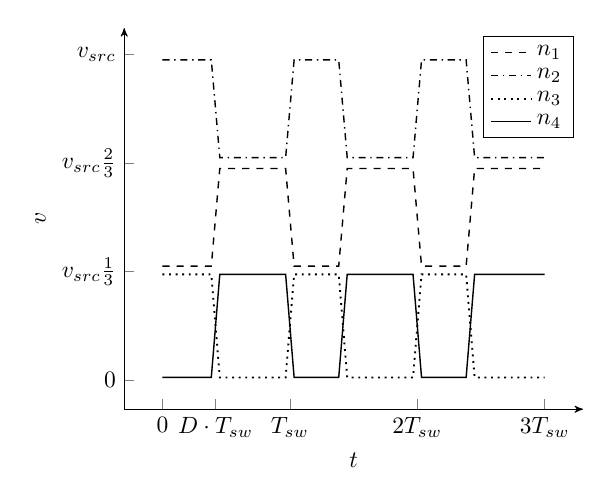
\begin{tikzpicture}[xscale=0.85, yscale=0.85]
    \begin{axis}[
        xlabel near ticks,
        xlabel=$t$,
        ylabel=$v$,
        axis line style={->},
        axis y line*=left,
        axis x line*=bottom,
        ytick = {0,2,4,6},
        yticklabels={0,$v_{src}\frac{1}{3}$,$v_{src}\frac{2}{3}$,$v_{src}$},
        xtick = {0,1.25,3,6,9},
        xticklabels={0,$D \cdot T_{sw}$,$T_{sw}$ ,$2 T_{sw}$,$3 T_{sw} $},
        ]

  %Vertical ticks
  %\draw (2pt,6) -- (-5pt,6) node[anchor=east]  {$v_{src} $};
  %\draw (2pt,4) -- (-5pt,4) node[anchor=east]  {$v_{src} \frac{2}{3}$};
  %\draw (2pt,2) -- (-5pt,2) node[anchor=east]  {$v_{src} \frac{1}{3}$};

  %Horizontal ticks
  %\draw (1.25,2pt) -- (1.25,-5pt) node[anchor=north]  {$DT$};
  %\draw (3,2pt) -- (3,-5pt) node[anchor=north]  {$T$};
  %\draw (6,2pt) -- (6,-5pt) node[anchor=north]  {$2T$};
  %\draw (9,2pt) -- (9,-5pt) node[anchor=north]  {$3T$};
  %\draw (0,0) node[anchor=north east]  {$0$};

  \addplot[semithick, dashed]
    plot coordinates{
        (0,2.1)   (1.15,2.1)  (1.35,3.9)  (2.9,3.9)
        (3.1,2.1) (4.15,2.1)  (4.35,3.9)  (5.9,3.9)
        (6.1,2.1) (7.15,2.1)  (7.35,3.9)  (9,3.9) };

  \addplot[semithick, dashdotted ]
    plot coordinates{
     (0,5.9)    (1.15,5.9)  (1.35,4.1)  (2.9,4.1)
     (3.1,5.9)  (4.15,5.9)  (4.35,4.1)  (5.9,4.1)
     (6.1,5.9)  (7.15,5.9)  (7.35,4.1)  (9,4.1)} ;

  \addplot[thick,dotted ]
    plot coordinates{
   (0,1.95)   (1.15,1.95)  (1.35,0.05)  (2.9,0.05)
   (3.1,1.95) (4.15,1.95)  (4.35,0.05)  (5.9,0.05)
   (6.1,1.95) (7.15,1.95)  (7.35,0.05)  (9,0.05)};

   \addplot[semithick]
    plot coordinates{
    (0,0.05)    (1.15,0.05)    (1.35,1.95)    (2.9,1.95)
    (3.1,0.05)  (4.15,0.05)  (4.35,1.95)  (5.9,1.95)
    (6.1,0.05)  (7.15,0.05)  (7.35,1.95)  (9,1.95) };

    \legend{$n_1$,$n_2$,$n_3$,$n_4$}


\end{axis}
\end{tikzpicture}
\caption{Transient voltage at the different \emph{pwm}-nodes of the 3:1 H-Dickson converter of Figure~\ref{fig:3_1_hscc}.}
\label{fig:pwm_nodes}
\end{SCfigure}
In the 3:1 H$^2$-Dickson there is actually a plurality of \emph{pwm}-nodes. Figure~\ref{fig:pwm_nodes} plots all the switching voltages available in the converter. The square-wave voltages are equally spaced to cover the range from 0 to $v_{src}$ with a voltage ripple of $v_{src}/3$. Being this equal spacing is unique of Dickson and Ladder compared to the other SCC topologies. In fact, the amplitude of the PWM voltages, so in the switching node $v_x,$ is fixed by the intrinsic conversion ratio $m_i$, hence
\begin{equation}
\Delta v_{x} = m_i v_{src}.
\label{eq:del_vx}
\end{equation}
%and the reason why these two topologies were selected to implement all the H-SCCs discussed in this dissertation
Notice that, a H-SCC shares many of the characteristics of a buck converter, which is the most common \emph{dc-dc} topology used as a LED driver. Adding the output filter to a SCC complements the converter by providing tight current regulation, which overcomes the intrinsic limitation of SCC in this respect. However, it requires magnetic elements, challenging the integrability  of the converter. The following sections introduce the characteristics of this new \emph{hybrid} topology as a LED driver, using the buck converter as a reference. %  since a H-SCC architecture can directly replace a buck converter LED driver providing the same regulation characteristics.

\subsection{Output Regulation}
\label{sec:out_reg}
In contrast with the classical SCC, the conversion ratio of a H-SCC converter can be adjusted. It actually depends on the duty cycle ($D$) of the driving signals, and consequently the conversion ratio can be adjusted to provide regulation to the load without directly affecting the converter's efficiency.

Figure~\ref{fig:reg_comp} compares the trend curves of the converter efficiency with respect to the conversion ratio for a three different converters a 3:1 H$^3$-Dickson, a 3:1 Dickson and a buck converter. For instance, the \emph{dc}-node of the 3:1 Dickson has an intrinsic conversion ratio of $m_i = \frac{1}{3} $, and it provides regulation at the cost of efficiency. Instead using the third \emph{pwm}-node ($n_3$) of the same Dikson converter of Figure~\ref{fig:3_1_hscc}, the converter has an adjustable conversion ratio given by
\begin{equation}
m_3 = \frac{D}{3}
\end{equation}
where $D$ is the duty cycle of the odd numbered switches. In this case the efficiency-regulation ($\eta$-$m_e$) curve is flat within the regulation margins, and drops for extreme duty cycles because of, not yet discussed\footnote{The details of the loss mechanisms in SCC and H-SCC are covered in Chapter~\ref{ch:modeling} dedicated to modeling.}, internal losses of the SCC stage. Furthermore, the $\eta$-$m_e$ curve of a H-SCC is similar to the one of a buck converter but with a smaller dynamic range.
\begin{SCfigure}[][!h]
\centering
\begin{circuitikz}[american,xscale=0.55,yscale=0.65]
\begin{scope}


  \draw [->] (0,0) -- (10,0) node[anchor=north]{$m_e$};
  \draw [->] (0,0) -- (0,5.5) node[anchor=east]{$\eta$};

  %Vertical ticks
  \draw (2pt,4) -- (-5pt,4) node[anchor=east]  {$100\%$};
  \draw (2pt,2.5) -- (-5pt,2.5) node[anchor=east]  {$70\%$};

  %Horizontal ticks
  %\draw (1.25,2pt) -- (1.25,-5pt) node[anchor=north]  {$DT$};
  \draw (3,2pt) -- (3,-5pt) node[anchor=north]  {$\frac{1}{3}$};
  \draw (6,2pt) -- (6,-5pt) node[anchor=north]  {$\frac{2}{3}$};
  \draw (9,2pt) -- (9,-5pt) node[anchor=north]  {$1$};
  \draw (0,0) node[anchor=north east]  {$0$};

  \draw[thick, dashed] (0,0) --  (2.9,3.9) ;

  %\draw[thick, dotted] (0,0) --  (2.9,3.9) ;
  \draw[thick,dotted] (0.1,2) parabola[bend at end] (2,3.45) -- (6,3.7) parabola[bend at start] (8.9,1.5);

  \draw[thick] (0.1,1.75) parabola[bend at end] (0.75,3.5) -- (2.2,3.6) parabola[bend at start] (2.9,1.6);

  \draw[thick] (4,5) -- (5,5) node[anchor=west,font=\small] {3:1 H$^3$-Dikson};
  \draw[thick,dashed] (4,4.5) -- (5,4.5) node[anchor=west,font=\small] { 3:1 Dickson };
  \draw[thick,dotted] (4,5.5) -- (5,5.5) node[anchor=west,font=\small] { Buck };
\end{scope}
\end{circuitikz}
\caption{Comparison of regulation-efficiency characteristics between converters.}
\label{fig:reg_comp}
\end{SCfigure}

\begin{table}[h]

\centering
\caption{Intrinsic conversion ratios, $m_i$, at the different nodes of a 3:1 H-Dickson converter.}
\label{tab:3:1 H-Dick_M}
\renewcommand{\arraystretch}{1.5}% Wider
\begin{tabular}{l  c | c c c c c }
 Node &  & $n_1$ & $n_2$ & $n_3$ & $n_4$ & $n_{dc}$ \\
 \midrule
 Conversion ratio & $m_x$ & $\frac{2+D}{3} $    & $\frac{2-D}{3} $ & $\frac{D}{3} $ & $\frac{1-D}{3} $ & $\frac{1}{3}$ \\
 Range of conversion &       & $1 \cdots \frac{2}{3}$ & $\frac{2}{3} \cdots \frac{1}{3} $ & $0 \cdots \frac{1}{3}$ & $0 \cdots  \frac{1}{3} $ & - \\
 Dynamic conversion range & $\Delta m$ &  $\frac{1}{3}$ &  $\frac{1}{3}$ &  $\frac{1}{3}$ &  $\frac{1}{3}$ &  -
\end{tabular}
\end{table}

Ideally a buck converter provides a conversion ratio between 0 and 1. Indeed, it is the same case for a H-SCC, however the conversion ratio is segmented in different ranges. Each segment is associated with a different \emph{pwm}-node of the converter, and it has a limited dynamic range of regulation $\Delta m$. Table~\ref{tab:3:1 H-Dick_M} presents the conversion characteristics for the different nodes of the 3:1 H-Dickson of Figure~\ref{fig:3_1_hscc}. It can be seen that the dynamic range of conversion ($\Delta m$) is the same across all the \emph{pwm}-nodes and equal to the intrinsic conversion ratio of the converter $m_i$. This characteristic is also shared between the two topologies used in this dissertation, Dickson and Ladder.

\subsection{Power Inductor}
\label{ch:power_inductor}

Like in a buck converter, a H-SCC uses a inductor-capacitor (LC) low pass filter to supply the \emph{dc} voltage to the load. The use of an inductor challenges the integrability of the converter, as was already discussed in the second chapter, nevertheless the added advantages in terms of regulation and efficiency justify its use. At the same time, the inductor benefits from the reduced voltage excursion present on the \emph{pwm}-nodes, relaxing its requirements in terms of inductance and size.
\begin{figure}[!h]
\centering
\ctikzset { bipoles/length=1cm}
\begin{subfigure}[t]{.45\textwidth}
    %\centering
    \raggedright
    \begin{circuitikz} [american voltages,scale=0.65]
    \draw
        (-1,0) to[V = $v_{src}$]
        (-1,4) -- (1,4) to[gswitch,l=$s_1$]
        (1,2) -- (1.5,2) to[inductor=${l_o}$,i=$i_o$]
        (3.5,2) -- (4,2) to[C,l=$c_o$] (4,0) -- (-1,0);

    \draw (4,2) to[short,-o] (5,2) node[anchor=west] {$v_o$};

    \draw (1,2) to[gswitch,l=$s_2$] (1,0);

    \draw (1,2) node[anchor=east] {$v_x$};

    \draw (0,-1) node[anchor=south] {};

    \end{circuitikz}
    \caption{}
    \label{fig:ind_ckt_l}
\end{subfigure}
\begin{subfigure}[t]{.45\textwidth}
    %\centering
    \raggedleft
    \begin{circuitikz} [scale=0.65]
    \begin{scope}%[xshift = 8cm, yshift=0cm]
        \draw[->] (0,0) -- (6.25,0) node[anchor=north] {$  t $};
        \draw[->] (0,0) -- (0,3.2) node[anchor= east] {$v_x $};

        %Ticks X
        \draw (2.75,2pt) -- (2.75,-5pt) node[anchor=north] {$T$};
        \draw (5.5,2pt) -- (5.5,-5pt) node[anchor=north] {$2T$};

        %Ticks Y
        \draw (2pt,2.5) -- (-5pt,2.5) node[anchor=east] {$v_{src}$};
        \draw (0,0) node[anchor=north east] {$0$};


        \draw[thick] (0,2.5) -- (1.25,2.5) -- (1.25,0) -- (2.75,0) -- (2.75,2.5) -- (4,2.5) -- (4,0) -- (5.5,0);
        \draw (0,-1) node[anchor=south] {};

        \draw[pil,<->] (4.75,-0.1) -- (4.75,2.6);
        \draw (4.75,1.25) node[anchor=west] {$\Delta v_x$};
        \draw[dotted] (4,2.5) -- (4.95,2.5);

    \end{scope}
    \end{circuitikz}
    \caption{}
\label{fig:induc_vx}
\end{subfigure}
\caption{Inductor based converter, \emph{left} - synchronous buck converter schematic; \emph{right} - transient voltage at the switching node during two switching periods. }
\label{fig:inductive_smps}
\end{figure}

The inductance value of the power inductor in a buck type converter configuration is
\begin{equation}
 l_{o}   = \frac{\Delta v_{x} ~ D (1-D)}{\Delta i ~ f_{sw}},
\label{eq:gen_l}
\end{equation}
where $\Delta i$ is the \emph{peak-to-peak} current amplitude in the inductor, $D$ the duty cycle of the buck high side switch. From~\eqref{eq:gen_l} it can be seen that the size of the power inductor is directly proportional to the amplitude of the square-wave voltage at the switching node ($\Delta v_x$), while for a buck converter it is equal to the source voltage, as shown in the plot from Figure~\ref{fig:induc_vx}. Specifying~\eqref{eq:gen_l} for a buck converter, gives
\begin{equation}
 l_{o,buck}  = \frac{v_{src} ~ D(1-D)}{\Delta i ~ f_{sw} }.
\label{eq:buck_l}
\end{equation}

Contrary to the buck converter, in the H-SCC the square-wave voltages are floating with respect the ground (see Figure~\ref{fig:vx_t}) and its ripple amplitude $\Delta v_x$ depends on the converter's topology. In the case of the Dickson and Ladder converters the amplitude of the voltage ripple $\Delta v_x$ is the same for all of the \emph{pwm}-nodes and equal to
\begin{equation}
 \Delta v_x   = m_i \cdot v_{src},
\label{eq:h_scc_Del_vx}
\end{equation}
therefore specifying~\eqref{eq:gen_l} for a Dickson or a Ladder H-SCC, gives
\begin{equation}
 l_{o,hscc}  = \frac{ m_i \cdot v_{src} \cdot D (1-D)}{\Delta i f_{sw} }.
\label{eq:hscc_l}
\end{equation}

An important remark is that the duty cycles $D$ in~\eqref{eq:hscc_l} and in~\eqref{eq:buck_l} are not correlated, therefore the two equations can not be directly compared.  Figure~\ref{fig:inductor_size} plots the normalized\footnote{Normalization given for $v_{src} = 1V$, $T_{sw}=1s$ and $\Delta i = 1A$.} inductor values for Buck, 3:1 H-Dickson and 4:1 H-Dickson converters. The plot shows a concave function for the buck converter where the highest inductance value is when the converter operates at $50\%$ conversion ratio. In contrast, the curves corresponding to H-SCCs present multiple concave peaks, where each of them corresponds to a selected node of the HSCC converter. For instance, looking at the dashed line plotted for the 3:1 H-Dickson converter of Figure~\ref{fig:3_1_hscc}, the first parabola spans $m$ between $0$ and $1/3$, where an inductor is connected to $n3$ or $n4$. The second parabola spans $m$ between $1/3$ and $2/3$, where an inductor is connected to $n2$. The last parabola spans $m$ between $2/3$ and $1$, where the inductor is connected to $n1$.
\begin{SCfigure}[][!h]
\centering
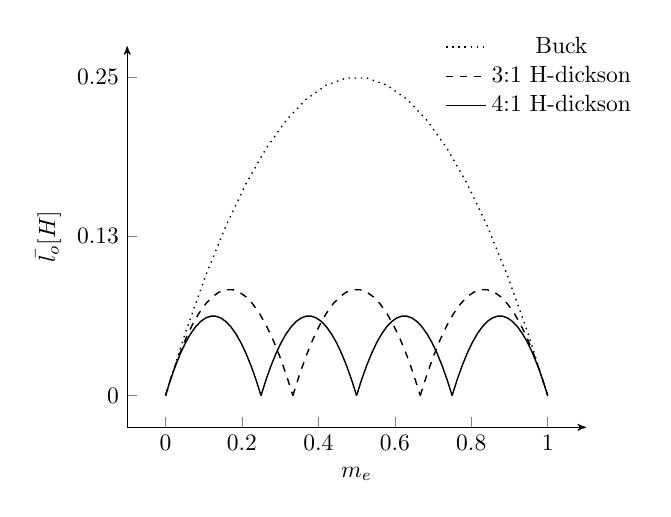
\begin{tikzpicture}[scale=0.85]
    \begin{axis}[
        xlabel near ticks,
        xlabel=$m_e$,
        ylabel={$\bar{l_o}  [ H ]  $} ,
        axis line style={->},
        axis y line*=left,
        axis x line*=bottom,
        ytick = {0,.125,.25},
        %yticklabels={0,$v_{src}\frac{1}{3}$,$v_{src}\frac{2}{3}$,$v_{src}$},
        domain=0:1,
        samples=20,
        %xticklabels={0,$D \cdot T_{sw}$,$T_{sw}$ ,$2 T_{sw}$,$3 T_{sw} $},
        legend style={at={(1.125,1.05)}, anchor= north east,draw=none},
        ]

  \addplot [semithick,dotted] {x*(1-x)};
  \addplot [domain = 0:1/3,  semithick,dashed]   {1/3* (x*3)*(1-(x*3))};
  \addplot [domain = 0:1/4,    semithick]   {1/4* (x*4)*(1-(x*4))};

  \addplot [domain = 1/3:2/3,semithick,dashed] {1/3* (2-x*3)*(1-(2-x*3))};
  \addplot [domain = 2/3:1,  semithick,dashed]   {1/3* (x*3-2)*(1-(x*3-2))};


  \addplot [domain = 1/4:2/4,  semithick]   {1/4* (x*4 - 1)*(1-(x*4 - 1))};
  \addplot [domain = 2/4:3/4,  semithick]   {1/4* (3 - x*4)*(1-(3 - x*4))};
  \addplot [domain = 3/4:4/4,  semithick]   {1/4* (x*4-3)*(1-(x*4-3))};

  \legend {Buck, 3:1 H-dickson,4:1 H-dickson};
\end{axis}
\end{tikzpicture}
\caption{Inductance value for Buck, 3:1 H-Dickson and 4:1 H-Dickson converters as function of the conversion ratio; results are normalized  for $V_{src} = 1V$, $T_{sw}=1s$ and $\Delta i = 1A$.}
\label{fig:inductor_size}
\end{SCfigure}

The reduction in inductance value with respect to the buck converter spans out from $50\%$ conversion ratio to the extremes where the inductance takes the same values for all the converters. The physical size of the inductor is proportional to the peak energy stored in it, and it can be computed from the maximum current through the inductor
\begin{equation}
 E_{l,max}  = \frac{1}{2} i_{max}^2 l_{o}.
\label{eq:eng_L}
\end{equation}
The minimum inductance value occurs when the converter operates in boundary conduction mode (BCM) for converters designed to operate continuous conduction mode (CCM), as is the case of the H-SCC. When a buck or H-SCC converter operates in BCM, the minimum current is equal to zero and the peak current is equal to twice of the output current of the converter. Thus, the maximum inductor current is
\begin{equation}
 i_{max} = \Delta i  = 2 i_{out}
\label{eq:i_max}
\end{equation}
By substituting (\ref{eq:i_max}) and (\ref{eq:buck_l}) into (\ref{eq:eng_L}), the inductor peak energy for a buck can be found
\begin{equation}
E_{l,buck}  =   \frac{ i_{out} v_{src}  D(1-D)}{f_{sw}}.
\label{eq:e_lmax_buck}
\end{equation}
\begin{SCfigure}[][!h]
\centering
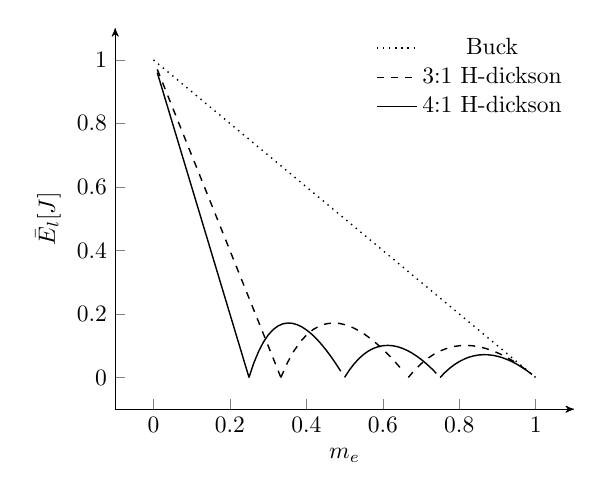
\begin{tikzpicture}[scale=0.85]
    \begin{axis}[
        xlabel near ticks,
        xlabel=$m_e$,
        ylabel={$\bar{E}_{l} [ J ]  $} ,
        axis line style={->},
        axis y line*=left,
        axis x line*=bottom,
        %ytick = {0,.125,.25},
        %yticklabels={0,$v_{src}\frac{1}{3}$,$v_{src}\frac{2}{3}$,$v_{src}$},
        domain=0:1,
        samples=20,
        %xticklabels={0,$D \cdot T_{sw}$,$T_{sw}$ ,$2 T_{sw}$,$3 T_{sw} $},
        legend style={at={(1,1)}, anchor= north east,draw=none},
        ]

  \addplot [semithick,dotted] {(1-x)};
  \addplot [domain = 0.01:1/3, semithick, dashed]   {1/x* 1/3* (x*3)*(1-(x*3))};
  \addplot [domain = 0.01:1/4, semithick]   {1/x* 1/4* (x*4)*(1-(x*4))};

  \addplot [domain = 1/3:2/3-0.01,semithick,dashed] {1/x*1/3* (2-x*3)*(1-(2-x*3))};
  \addplot [domain = 2/3:1-0.01,  semithick,dashed]   {1/x*1/3* (x*3-2)*(1-(x*3-2))};


  \addplot [domain = 1/4:2/4-0.01,  semithick]   {1/x*1/4* (x*4 - 1)*(1-(x*4 - 1))};
  \addplot [domain = 2/4:3/4-0.01,  semithick]   {1/x*1/4* (3 - x*4)*(1-(3 - x*4))};
  \addplot [domain = 3/4:4/4-0.01,  semithick]   {1/x*1/4* (x*4-3)*(1-(x*4-3))};

  \legend {Buck, 3:1 H-dickson,4:1 H-dickson};
\end{axis}
\end{tikzpicture}
\caption{Peak energy storage for Buck, 3:1 H-Dickson, and 4:1 H-Dickson converters as function of the conversion ratio;  results are normalized for $P_{out} = 1W$ and $f_{sw}=1Hz$.}
\label{fig:inductor_energy}
\end{SCfigure}
In a buck converter the source voltage can be written as
\begin{equation}
v_{src}  =  \frac{v_{out}} {D},
\label{eq:vo_buck}
\end{equation}
thus by substituting (\ref{eq:vo_buck}) into (\ref{eq:e_lmax_buck}), the $E_{l,buck}$ yields to
\begin{equation}
E_{l,buck}  =  \frac{v_{vout}}{D} \frac{ i_{out}  D(1-D)}{f_{sw}} = \frac{(1-D)}{f_{sw}} P_{out}.
\label{eq:e_lmax_buck_II}
\end{equation}
By substituting (\ref{eq:i_max}) and (\ref{eq:hscc_l}) into (\ref{eq:eng_L}), the inductor peak energy for a H-SCC using Dickson or Ladder stages can be found
\begin{equation}
E_{l,hscc}  =   \frac{ m_{i} ~ i_{out} ~ v_{src} ~ D(1-D)}{f_{sw}}.
\label{eq:e_lmax_hscc}
\end{equation}
Rearranging~\eqref{eq:eff_m} $v_{src}$ can be written as function of the \emph{effective} conversion ratio, as
\begin{equation}
v_{src}  =  \frac{v_{out}} {m}.
\label{eq:vo_hscc}
\end{equation}
Subsequently, by substituting (\ref{eq:vo_hscc}) into (\ref{eq:e_lmax_hscc}), the resulting expression of the inductor maximum energy yields to
\begin{equation}
E_{l,hscc}  =  \frac{v_{vout}}{m_e} \frac{ m_i ~i_{out} ~ D(1-D)}{f_{sw}} = \frac{m_i~ D (1-D)}{m_e~ f_{sw}} P_{out}.
\label{eq:e_lmax_hscc_II}
\end{equation}

Figure~\ref{fig:inductor_energy} plots (\ref{eq:e_lmax_buck_II}) and (\ref{eq:e_lmax_hscc_II}), both plots have the same trend of reducing the peak energy as the conversion ratio increases. With regard to the inductance value (see Figure~\ref{fig:inductor_size}), the peak energy stored in the inductor, and hence the volume, are dramatically reduced in case of using a H-SCC topology; as shown in Figure~\ref{fig:inductor_normal}. The plot shows that the reduction in inductance volume ranges from a conversion ratio of $50\%$ to the extremes $0\%$ and $100\%$ symmetrically, being very effective in most of the conversion ratio range of the converter and decreasing at the two extremes. As the intrinsic conversion ratio $m_i$ of the SCC stages decreases, the reduction in inductance increases, and  the effective region spans for a larger range of conversion ratios.
\begin{SCfigure}[][!h]
\centering
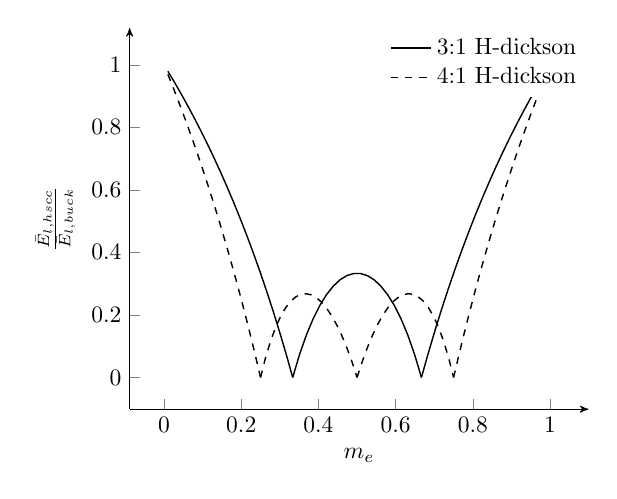
\begin{tikzpicture}[scale=0.85]
    \begin{axis}[
        xlabel near ticks,
        xlabel=$m_e$,
        ylabel={$ \frac{\bar{E}_{l,hscc}}{\bar{E}_{l,buck}}  $} ,
        axis line style={->},
        axis y line*=left,
        axis x line*=bottom,
        %ytick = {0,.125,.25},
        %yticklabels={0,$v_{src}\frac{1}{3}$,$v_{src}\frac{2}{3}$,$v_{src}$},
        domain=0:1,
        samples=20,
        %xticklabels={0,$D \cdot T_{sw}$,$T_{sw}$ ,$2 T_{sw}$,$3 T_{sw} $},
        legend style={at={(1,1)}, anchor= north east,draw=none},
        ]


  \addplot [domain = 0.01:1/3,  semithick]   { (1/x* 1/3* (x*3)*(1-(x*3)))/(1-x) };
  \addplot [domain = 0.01:1/4,    semithick,dashed]   { (1/x* 1/4* (x*4)*(1-(x*4)))/(1-x)};

  \addplot [domain = 1/3:2/3,semithick] { (1/x*1/3* (2-x*3)*(1-(2-x*3)))/(1-x)};
  \addplot [domain = 2/3:1,  semithick]   { (1/x*1/3* (x*3-2)*(1-(x*3-2)))/(1-x)};


  \addplot [domain = 1/4:2/4,  semithick,dashed]   { (1/x*1/4* (x*4 - 1)*(1-(x*4 - 1)))/(1-x)};
  \addplot [domain = 2/4:3/4,  semithick,dashed]   { (1/x*1/4* (3 - x*4)*(1-(3 - x*4)))/(1-x)};
  \addplot [domain = 3/4:4/4,  semithick,dashed]   { (1/x*1/4* (x*4-3)*(1-(x*4-3)))/(1-x)};

  \legend {3:1 H-dickson,4:1 H-dickson};
\end{axis}
\end{tikzpicture}
\caption{Peak energy storage normalized with respect to a buck converter for a 3:1 H-Dickson and a 4:1 H-Dickson converters as function of the conversion ratio.}
\label{fig:inductor_normal}
\end{SCfigure}

\subsection{Power Switches}
The large number of switches used in a H-SCC has different advantages with regards to miniaturization of the converter. In fact, in a H-SCC the voltage stress applied to the different switches is a fraction of the input voltage, in contrast to the buck converter where each of the switches have to block the full input voltage. Therefore SCCs can be implemented with switches rated at lower voltages than the input voltage. Reducing the voltage stress at the switches has the following advantages:
\begin{itemize}
  \item Low voltage devices take less silicon area in the standard integration processes.
  \item Switching performance is better since the lower voltages switches are smaller in area, and they have less parasitic capacitances, as a consequence they can switch faster.
  \item Switching losses of the converter are reduced since they have a quadratic relationship with the blocking voltages of the switches ($v_{ds}$).
\end{itemize}
From the three above-mentioned advantages, the two first facts are mainly technology-related hence their benefits are not trivial to be quantified. In contrast, the last fact can be assumed to be technology-independent and easily quantified. By assuming that drain-source capacitance $c_{ds}$ is a constant among different devices and technologies, the switching losses can be computed and compared with respect to the buck.
\begin{table}[h]
\centering
\caption{Stress voltages at the switches of the 3:1 H-Dickson of Figure~\ref{fig:3_1_hscc}.}
\label{tab:3:1 H-Dick_V_stress}
\renewcommand{\arraystretch}{1.5}% Wider
\begin{tabular}{r  c}
 Switch & $v_{ds}$  \\
 \midrule
 $s_1,s_3 \cdots s_7$ & $\frac{1}{3} v_{src}$ \\
 $s_2$ & $\frac{2 }{3} v_{src}$
\end{tabular}
\end{table}


Switching losses are given by~\cite{2001Erickson}
\begin{equation}
P_{sw} = \frac{1}{2} f_{sw} \cdot c_{ds} \cdot v_{ds}^2.
\label{eq:p_sw_dev}
\end{equation}
In a buck converter of Figure~\ref{fig:ind_ckt_l} the blocking voltage of the switches is $v_{src}$, thus using~\eqref{eq:p_sw_dev} the switching losses result in
\begin{equation}
P_{sw,buck} =   f_{sw} \cdot c_{ds} \cdot v_{src}^2.
\label{eq:p_sw_buck}
\end{equation}
The blocking voltages of the 3:1 H-Dickson are shown in Table~\ref{tab:3:1 H-Dick_V_stress}.  Applying~\eqref{eq:p_sw_dev} the switching losses for the converter can be formulated, resulting in
\begin{equation}
P_{sw,hscc} =  \frac{6}{2}  f_{sw} \cdot c_{ds} \left( \frac{1}{3} v_{src} \right)^2 + \frac{1}{2}  f_{sw} \cdot c_{ds} \left( \frac{2}{3} v_{src} \right)^2 ,
\label{eq:p_sw_hscc}
\end{equation}
rearranging~\eqref{eq:p_sw_hscc},  yields to
\begin{equation}
P_{sw,hscc} =  \frac{5}{9}  f_{sw} \cdot c_{ds} \cdot v_{src}^2.
\label{eq:p_sw_hscc_sol}
\end{equation}
By dividing~\eqref{eq:p_sw_buck} and~\eqref{eq:p_sw_hscc_sol}, we can obtain  the ratio between the two converters
\begin{equation}
\frac{P_{sw,hscc}}{P_{sw,buck}} =  \frac{5}{9}.
\label{eq:p_sw_rel}
\end{equation}
The result shows that using a H-SCC we can achieve a reduction of the switching losses of almost one half with respect to the buck converter, even when the H-SCC converter is using five more switches than the buck converter. Applying~\eqref{eq:p_sw_dev} with the blocking voltages defined for the N:1 Dickson and Ladder converters in Table~\ref{tab:Dick_Ladder_v_blk}, the formulation of the switching losses can be generalized, resulting in
\begin{align}
P_{sw,dickson} & =  \frac{4+N}{8 \cdot N^2} \cdot v_{vin}^2 \cdot f_{sw}  \cdot {c_{ds}} , \\
P_{sw,ladder}  & =  \frac{1}{ N} \cdot v_{src}^2 \cdot f_{sw} \cdot {c_{ds}}    .
\label{eq:p_sw_gen}
\end{align}
Normalizing them with respect to the power losses of the buck converter~\eqref{eq:p_sw_buck}, yields
\begin{align}
\bar{P}_{sw,dickson} & = \frac{4+N}{8 \cdot N^2} ,\label{eq:n_sw_dick}\\
\bar{P}_{sw,ladder} & = \frac{1}{ N}. \label{eq:n_sw_lddr}
\end{align}
\begin{table}[h]
\centering
\caption{Switch blocking voltage of Dickson and Ladder converters.}
\label{tab:Dick_Ladder_v_blk}
\renewcommand{\arraystretch}{1.5}% Wider
\begin{tabular}{r | c  c   }
 Converter &  N:1 Dickson  $ N \geq$ 3  &  N:1 Ladder $ N \geq 2$  \\
 \midrule
\# Switches & $ 4 + N $  & $2 \cdot N$ \\
 $v_{ds}$ &     $\begin{array} {rcl} 6   & \to &  \frac{v_{src}}{N} \\
                                     (N - 2) & \to & \frac{2 v_{src}}{N}
                 \end{array}$
          &  $\frac{v_{src}}{N} $ \\
\end{tabular}
\end{table}

Figure~\ref{fig:psw_ratio} plots~\eqref{eq:n_sw_dick} and~\eqref{eq:n_sw_lddr}, showing the switching loss ratio with respect to the buck converter. It can be seen that both converters reduce the switching losses with respect to the buck converter. In fact, as $N$ increases to losses decrease, although the number of switches increase as well. Reducing the switching loss will enable to operate the converter at higher frequencies, thus with a smaller switching period $T_{sw}$, which is also effective in the reduction of the power inductor.

\begin{SCfigure}
\centering
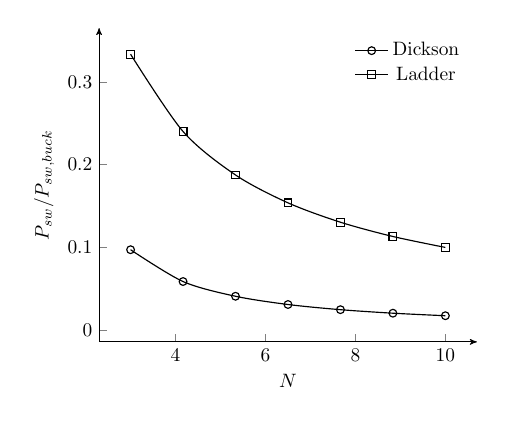
\begin{tikzpicture}[scale=0.7]
    \begin{axis}[
        xlabel near ticks,
        xlabel=$N$,
        ylabel=$P_{sw}/P_{sw,buck}$,
        axis line style={->},
        axis y line*=left,
        axis x line*=bottom,
        domain=3:10,
        samples=7,
        legend style={
                draw=none,}
        ]
  %\addplot [semithick] {x*0+1};
  \addplot [semithick,smooth,mark=o,mark size=2,scale plot marks=false] {(4+x)/(8*x^2)};
  \addplot [semithick,smooth,mark=square, mark size=2 ,scale plot marks=false]{1/x};
  \legend {Dickson,Ladder};
\end{axis}
\end{tikzpicture}
\caption{Switching loss ratio for Dickson and Ladder converters with respect to the buck converter.}
\label{fig:psw_ratio}
\end{SCfigure}

The lecture of the results is given from a qualitative perspective, consequently a couple of considerations have to be pointed regarding a practical implementation of a H-SCC. First, they are obtained assuming that $c_{ds}$ is the same for all the switches in both converters. In a practical converter each device has a different $c_{ds}$ value defined by two of the device parameters; $c_{ds}$ is directly proportional to the rated $v_{ds}$  voltage and inversely proportional to the channel resistance $r_{on}$. Theoretically, lower voltage switches have smaller $c_{ds}$, but the final value will also depend on its $r_{on}$. Second, H-SCC has a larger number of devices in series in the current path compared to a buck, that only has only one switch in the current path in both phases. A proper H-SCC design reduces the number of switches in the high current path, helping to keep the conduction loss low. In order to provide a better understanding of the advantages that H-SCC offer, the last chapter of the dissertation provides a deeper analysis between converters.

\subsection{Multiple Outputs}
The use of the internal nodes of the SCC allows to provide multiple outputs with a single power train. For instance, the converter could be simultaneously loaded at the \emph{pwm}-nodes and at the \emph{dc}-node, providing different conversion ratios for each output. The conversion ratio at the \emph{dc}-node (or nodes)  is given by the intrinsic conversion ratio of the converter $m_i$, independent of the variations in the duty cycle of the driving signal, yet this fixed output can be linearly regulated to adjust the output voltage.  The conversion ratio for the other \emph{pwm}-nodes is a function of $D$ and determined for each node by the node conversion ration $m_n$. In the case of using multiple \emph{pmw}-nodes, all the outputs will depend on $D$, hence it will not be possible to have independent regulation for each of the outputs. This happens because in order to guarantee the proper operation of a SCC, all switches are associated to a phase, hence they can not be independently controlled.
\begin{figure}[!h]
\centering
\ctikzset { bipoles/length=1cm}
\begin{circuitikz}[american voltages,scale=0.65]
\draw
        %Draw Switches

        (0,0) node[sground]{} to[V=$v_{src}$]
        (0,8)  --
        (5,8)   to[gswitch,l_=$s_1$,]
        (5,6)   to[gswitch,l_=$s_2$]
        (5,4)   to[gswitch,l_=$s_3$]
        (5,2)   to[gswitch,l_=$s_4$]
        (5,0)  --
        (0,0)

        (5,6) to[short] (8,6) to[L,l=$l_o$] (12,6) to[C,l_=$c_o$] (12,3) node[sground]{}
        (11,6) -- (14,6) to[R,l_=$r_2$,v^=$v_{o2}$] (14,3) node[sground]{}

        (5,4) to[short]
        (9,4) to[R,l_=$r_1$,v^=$v_{o1}$] (9,0) -- (5,0)

%Draw Capacitors
        (5,2) --
        (3,2) to[C=$c_{fly}$]
        (3,6)--
        (5,6)

        (5,0) --
        (7,0) to[C,l=$c_{dc}$]
        (7,4)--
        (5,4);

\end{circuitikz}
\caption[Two output H-SCC]{2:1 H-SCC with two outputs; $r_1$ is supplied by the \emph{dc}-node and $r_2$ is supplied by the first \emph{pwm}-node.}
\label{fig:2:1hscc_dual_output}
\end{figure}

Figure~\ref{fig:2:1hscc_dual_output} shows a converter with two output voltages. One load $r_1$ is connected to the \emph{dc}-node with an output voltage approximated by
\begin{equation}
v_{o1} = \frac{1}{2} v_{src}.
\end{equation}
the other load $r_2$ is connected to the first \emph{pwm}-node with an output voltage function of $D$ as
\begin{equation}
v_{o2} = \frac{1+D}{2} v_{src}.
\end{equation}
The voltage $v_{o2}$ can be regulated by means of $D$.

\section{DC-DC LED Drivers}
The buck converter is one of the most used topologies for LED drivers in \emph{dc-dc} applications. It has an excellent current regulation and a continuous output current thanks to the inductor connected in series with the output, as shown in Figure~\ref{fig:ind_ckt_led_drv}.

\begin{figure}[!h]
\centering
\ctikzset { bipoles/length=1cm}
\begin{subfigure}[t]{.45\textwidth}
    %\centering
    \raggedright
    \begin{circuitikz} [american voltages,scale=0.65]
    \draw
        (-1,0) to[V = $v_{src}$]
        (-1,4) -- (1,4) to[gswitch,l_=$s_1$]
        (1,2) -- (1.5,2) to[inductor=${l_o}$,i=$i_o$]
        (3.5,2) -- (4,2) to[C,l_=$c_o$] (4,0) -- (-1,0);

    \draw (4,2) to[short] (5.5,2) to[leD*,v_=$v_o$] (5.5,0) -- (4,0);

    \draw (1,2) to[gswitch,l_=$s_2$] (1,0);

    \draw (1,2) node[anchor=east] {$v_x$};

    \draw (0,-1) node[anchor=south] {};

    \end{circuitikz}
    \caption{}
    \label{fig:ind_ckt_led_drv}
\end{subfigure}
\hfill
\begin{subfigure}[t]{.45\textwidth}
    %\centering
    \raggedleft
    \begin{circuitikz} [scale=0.65]
    \begin{scope}%[xshift = 8cm, yshift=0cm]
        \draw[->] (0,0) -- (6.25,0) node[anchor=north] {$  t $};
        \draw[->] (0,0) -- (0,3.2) node[anchor= east] {$v_x $};

        %Ticks X
        \draw (2.75,2pt) -- (2.75,-5pt) node[anchor=north] {$T$};
        \draw (5.5,2pt) -- (5.5,-5pt) node[anchor=north] {$2T$};

        %Ticks Y
        \draw (2pt,2.5) -- (-5pt,2.5) node[anchor=east] {$v_{src}$};
        \draw (0,0) node[anchor=north east] {$0$};


        \draw[thick] (0,2.5) -- (1.25,2.5) -- (1.25,0) -- (2.75,0) -- (2.75,2.5) -- (4,2.5) -- (4,0) -- (5.5,0);
        \draw (0,-1) node[anchor=south] {};

        \draw[pil,>-<] (4.78,1.65) -- (4.78,0.6);
        \draw (4.78,0.55) -- (4.78,1.85)node[anchor=west] {$\Delta v_f$};



        \draw[thick,dotted] (0,1.36) -- (6,1.36) ;
        \draw[thick,dotted] (0,0.9) -- (6,0.9) ;
        \draw[thick,dashed] (0,1.137) -- (6,1.137) node[anchor=west] {$\bar{v_o}$};

    \end{scope}
    \end{circuitikz}
    \caption{}
\label{fig:induc_vx_led_drv}
\end{subfigure}
\caption[Gswitching node in the buck]{\emph{Left} - buck based LED driver schematic; \emph{right} - transient voltage at the switching node(thick line), average output voltage (dashed line), and forward voltage limits (dotted lines). }
\label{fig:inductive_led_drv}
\end{figure}

It can be seen in Figure~\ref{fig:induc_vx_led_drv} that the voltage swing at the switching node ($v_x$) of a buck converter goes from ground to $v_{src}$ providing the full conversion ratio range, between 0 and 1. Actually, this regulation range is often much wider than the margins of variation in the LED's forward voltage, as shown in Figure~\ref{fig:induc_vx_led_drv}. The \emph{dashed} line represents the average output voltage $\bar{v_o}$, thus the LED's forward voltage $v_f$, and the dotted lines represent the forward voltage variation boundaries $\Delta v_f$, being them around $\pm10\%$. Previously, in Chapter~\ref{sc:LED_load} was given a detailed discussion about the characteristics of the LED as a load.

\begin{figure}[!h]
\centering
\ctikzset { bipoles/length=1cm}
\begin{subfigure}[t]{.45\textwidth}
    %\centering
    \raggedright
    \begin{circuitikz} [american voltages,scale=0.65]
    \draw[dotted] (1,4) -- (1,3.5);

    \draw (1,3.35) -- (0.5,3.35);
    \draw[dotted] (0.5,3.35) --  (-.25,3.35) -- (-.25,3);

    \draw
        (1,3.5) to[gswitch,l_=$s_2$]
        (1,2) -- (2,2) to[inductor=${l_o}$,i=$i_o$]
        (4,2) -- (4,2) to[C,l_=$c_o$] (4,0.5) node[sground]{};

    \draw (4,2) to[short] (5.5,2) to[leD*,v_=$v_o$] (5.5,0.5) node[sground]{};

    \draw (1,2) to[gswitch,l_=$s_3$] (1,0.5);
    \draw[dotted] (1,0.5) --  (1,0) ;

    \draw (1.75,2) -- (1.75,1.5);
    \draw[dotted] (1.75,1.5) -- (1.75,1);

    \draw (1,2) node[anchor=east] {$v_x$};

    \draw (0,-1) node[anchor=south] {};

    \end{circuitikz}
    \caption{}
    \label{fig:hscc_ckt_led_drv}
\end{subfigure}
\hfill
\begin{subfigure}[t]{.45\textwidth}
    %\centering
    \raggedleft
    \begin{circuitikz} [scale=0.65]
    \begin{scope}%[xshift = 8cm, yshift=0cm]
        \draw[->] (0,0) -- (6.25,0) node[anchor=north] {$  t $};
        \draw[->] (0,0) -- (0,3.2) node[anchor= east] {$v_x $};

        %Ticks X
        \draw (2.75,2pt) -- (2.75,-5pt) node[anchor=north] {$T$};
        \draw (5.5,2pt) -- (5.5,-5pt) node[anchor=north] {$2T$};

        %Ticks Y
        \draw (2pt,2.5) -- (-5pt,2.5) node[anchor=east] {$v_{src}$};
        \draw (2pt,1.67) -- (-5pt,1.67) node[anchor=east] {$v_{src} \frac{2}{3}$};
        \draw (2pt,0.83) -- (-5pt,0.83) node[anchor=east] {$v_{src} \frac{1}{3}$};
        \draw (0,0) node[anchor=north east] {$0$};


        \draw[thick] (0,1.67) -- (1.25,1.67) -- (1.25,0.83) -- (2.75,0.83) -- (2.75,1.67) -- (4,1.67) -- (4,0.83) -- (5.5,0.83);
        \draw (0,-1) node[anchor=south] {};

        \draw[pil,>-<] (4.78,1.65) -- (4.78,0.6);
        \draw (4.78,0.55) -- (4.78,1.85)node[anchor=west] {$\Delta v_f$};



        \draw[thick,dotted] (0,1.36) -- (6,1.36) ;
        \draw[thick,dotted] (0,0.9) -- (6,0.9) ;
        \draw[thick,dashed] (0,1.137) -- (6,1.137) node[anchor=west] {$\bar{v_o}$};

    \end{scope}
    \end{circuitikz}
    \caption{}
\label{fig:hscc_vx_led_drv}
\end{subfigure}
\caption[Gswitching node in the H-SCC]{\emph{Left} - switching node detail of a 3:1 H-Dickson based LED driver; \emph{right} - transient voltage at the switching node(thick line), average output voltage (dashed line), and forward voltage limits (dotted lines).  }
\label{fig:hscc_led_drv}
\end{figure}

The abrupt $v-i$ characteristics of the LEDs is an advantage for the reduced conversion range of the H-SCC. Contrary to the buck converter, the H-SCC has a smaller voltage swing in the switching node. Figure~\ref{fig:hscc_led_drv} shows that the voltage limits of the switching node in a H-SCC can accommodate these variations of the LED's forward voltage.  As previously described in Section~\ref{sec:out_reg}, the dynamic conversion range at the outputs depend on the intrinsic conversion ratio $m_i$ of the SCC stage, therefore this dynamic range can be adjusted to the requirements of the load.

%The following subsections present different LED drivers based on H-SCCs for \emph{dc-dc} and \emph{ac-dc}. The presented topologies are also suitable to supply other load types, specially when these require a reduced conversion margin.

\subsection{Single-stage \emph{dc-dc} with auxiliary output voltage}
\begin{figure}[!h]
\ctikzset { bipoles/length=1cm}
\centering
    \begin{circuitikz}[american voltages,scale=0.6]

    \draw
            %Input Supply
            (0,0)  to[V=$v_{src}$]
            %Draw Switches
            (0,10.5)  --
            (5,10.5)  to[gswitch=$s_1$] %node[anchor=west] {$n_1$}%S1
            (5,9)  to[gswitch=$s_2$] %node[anchor=east] {$n_2$}%S1
            (5,7.5)  to[gswitch=$s_3$] %node[anchor=east] {$n_3$}%S1
            (5,6)   to[gswitch=$s_4$] %node[anchor=west] {$n_4$}%S2
            (5,4.5)   to[gswitch=$s_5$] %node[anchor=west] {$n_5$}%S3
            (5,3) --
            %left branch
            (3,3)   to[gswitch=$s_9$]
            (3,1.5)   to[gswitch=$s_8$]
            (3,0);

    \draw   %right branch
            (5,3) --
            (7,3)   to[gswitch,l_=$s_6$]
            (7,1.5)   to[gswitch,l_=$s_7$]
            (7,0) -- (0,0);



    \draw %Capacitor C1
           (2,6)
            to[pC,l_=$c_1$] (2,9) --
           (5,9);

    \draw %Capacitor C2
           (8.25,4.5)  to[pC,l_=$c_2$](8.25,7.5) --
           (5,7.5);

    \draw %Capacitor C3
           (3,1.5) -- (2,1.5)
            to[pC,l_=$c_3$] (2,6) --
           (5,6);

    \draw %Capacitor C4
           (7,1.5) --
           (8.25,1.5) -- (8.25,3) to[pC,l_=$c_4$](8.25,4.5) --
           (5,4.5);


    \draw  %LC output filter &  Output LED string
            (8.25,7.5)node[anchor=south] {$v_x$} to[L=$l_o$] (14,7.5)
            (13.5,0) to[pC,l=$c_{o}$] (13.5,7.5) -|
            (16,7.5) -- (16,7)  to[leD*] (16,5) to[leD*] (16,3) to[leD*] (16,1)   |- (7,0) ;

    %Vout label
    \draw (16.25,8.5) to[open,v^=$v_{out}$] (16.25,-1);

    \draw %Capacitor C3
           (5,0) to[pC,l_=$c_5$] (5,3) ;% node[anchor=south east] {$n_{dc}$};

     %\draw (7,4) to[short,-o] (10,4) node[anchor=west] {};
     %\draw (7,0) to[short,-o] (12,0) node[anchor=west] {};


     \draw (7,3) --([hs]8.25,4 |- 7,3) arc(180:0:\radius) to[short,-o] (10,3) to[open,v^=$v_{aux}$] (10,0) ;


     \end{circuitikz}
 \caption[5:1 H$^2$-Dickosn 12W LED driver]{ 5:1 H$^2$-Dickson LED driver for 24V e-merge track lighting application. The driver has two outputs: A $12V$, $12W$  LED string, and $4V$, $200mW$  to supply low power auxiliary loads. }
 \label{fig:5_1_hscc_emerge}
\end{figure}
Figure~\ref{fig:5_1_hscc_emerge} shows the \emph{dc-dc} LED driver with an auxiliary output voltage~\cite{WO2015/040564} used in the experimental set-up as a proof of concept for this dissertation, being presented in Chapter 5. The converter features two outputs: The main output $v_{out}$ supplies the LED load and normally delivers the largest amount of power. The output voltage can be controlled using the duty cycle $D$, thus its value is given by
\begin{equation}
v_{out} =  v_{src}  \frac{4 - D }{5}.
\label{eq:dc_dc_vout}
\end{equation}
The secondary output $v_{aux}$ supplies the low voltage electronics dedicated to the control of the driver, providing functionalities such as connectivity, light control and stand-by operation. The secondary output has no direct means of regulation and provides a fix conversion ratio equal to
\begin{equation}
v_{aux} =  v_{src} \frac{1 }{5}.
\label{eq:dc_dc_vaux}
\end{equation}
Nevertheless, the voltage at this output can still be controlled by means of a linear regulator.
\begin{figure}[!h]
\ctikzset { bipoles/length=1cm}
\centering
    \begin{circuitikz}[american voltages,scale=0.6]

    \draw
            %Input Supply
            (0,0)  to[V=$v_{src}$]
            %Draw Switches
            (0,10.5)  --
            (5,10.5)  to[gswitch=$s_1$] %node[anchor=west] {$n_1$}%S1
            (5,9)  to[gswitch=$s_2$]    %node[anchor=east] {$n_2$}%S1
            (5,7.5)  to[gswitch=$s_3$]  %node[anchor=east] {$n_3$}%S1
            (5,6)   to[gswitch=$s_4$]   %node[anchor=west] {$n_4$}%S2
            (5,4.5)   to[gswitch=$s_5$] %node[anchor=west] {$n_5$}%S3
            (5,3) --
            %left branch
            (3,3)   to[gswitch=$s_9$]
            (3,1.5)   to[gswitch=$s_8$]
            (3,0);

    \draw   %right branch
            (5,3) --
            (7,3)   to[gswitch,l_=$s_6$]
            (7,1.5)   to[gswitch,l_=$s_7$]
            (7,0) -- (0,0);



    \draw %Capacitor C1
           (2,6)
            to[pC,l_=$c_1$] (2,9) --
           (5,9);

    \draw %Capacitor C2
           (8.25,4.5)  to[pC,l=$c_2$](8.25,7.5) --
           (5,7.5);

    \draw %Capacitor C3
           (3,1.5) -- (2,1.5)
            to[pC,l_=$c_3$] (2,6) --
           (5,6);

    \draw %Capacitor C4
           (7,1.5) --
           (8.25,1.5) -- (8.25,3) to[pC,l=$c_4$](8.25,4.5) --
           (5,4.5);


    \draw  %LC output filter &  Output LED string
            (12,7.5)node[anchor=south west] {$v_x$} to[L=$l_o$] (15.5,7.5)
            (15,0) to[pC,l=$c_{o}$] (15,7.5) -|
            (16.5,7.5) -- (16.5,7)  to[leD*] (16.5,5) to[leD*] (16.5,3) to[leD*] (16.5,1)   |- (7,0) ;

            %Mux
    \draw   (12,7.5) -- (12,8.5) -- (11,9) -- (11,6) -- (12,6.5) -- (12,7.5)
            (11.5,7.5) node[rotate=90] {$mux$}
            (11.5,8.75) -- (11.5,9.5) node[anchor=west, rotate=90] {$sel$};

    \draw    %Mux connections
            (5,9)  --  (10,9) |- (11,8.5)
            (8.25,7.5)  --  (11,7.5)
            (5,6) --  (6.5,6) -- ([vs_d]5,7.5 -| 6.5,8 ) arc(270:90:\radius) --  (6.5,8) -- (11,8)
            (8.25,4.5) -| (9.5,7) -- (11,7)
            (8.25,1.5) -| (10,6.5) -- (11,6.5);

    %Vout label
    \draw (17,9) to[open,v^=$v_{out}$] (17,-1);

    \draw %Capacitor C3
           (5,0) to[pC,l_=$c_5$] (5,3) ;% node[anchor=south east] {$n_{dc}$};

     \end{circuitikz}
 \caption[5:1 H-Dickson LED driver 24V-12V-4V 12W LED driver]{ 5:1 H-Dickson LED driver with a multiplexer that enables to connect the different switching nodes with the power inductor.  }
 \label{fig:5_1_hscc_mux}
\end{figure}

\subsection{Single-stage \emph{dc-dc} with extended conversion range }

The reduced voltage swing at $v_x$, on the one hand favors in the reduction of output inductor, but on the other hand shrinks the conversion to a narrow range between $3/5$ and $4/5$. Using the same topology, the conversion ratio of the converter can be extended to the full range between 0 and 1, like in a buck converter, introducing a multiplexer~\cite{WO2015/040517} between the different floating \emph{pwm}-nodes and the power inductor as shown in Figure~\ref{fig:5_1_hscc_mux}. With this enhancement the power inductor can now be connecter to any of the available \emph{pwm}-nodes of the SCC stage.
%A detailed description of this architecture can be found in the annex X section Y.


\section{Summary}

In this chapter the hybrid switched capacitor converter (H-SCC) was introduced. First, the main operation and performance characteristics of the SCC were presented, with special emphasis on the limitations that these converters have with respect to load  regulation.

Subsequently, the H-SCC was described as a combination of SCC with an inductor. Such a \emph{hybrid} combination makes it possible to achieve a much better regulation than possible with the pure SCCs. In fact, the regulation enhancements in the H-SCC make the converter comparable to an inductive converters, especially to the buck. For that reason, two metrics were presented in order to qualitatively evaluate the benefits of these converters with respect to integration. These metrics shown that when using a H-SCC the inductor size and switching losses can be reduced compared to a buck converter.

Finally, the last section was dedicated to exploring the possibilities of the H-SCCs for LED driving. Different driver architectures for \emph{dc-dc} applications were presented, introducing the architecture that was used in the final demonstrator if this disoperation.

In conclusion, the H-SCC is a new power converter topology composed of a SCC and an inductor. The SCC implements the power train structure, where the SCC's conversion ratio adds a new variable to the design of the converter. Modifying this variable allows to adjust the voltages stress if the switches, capacitors, and inductors, and favors the integrability of the converter. At the same time, the extra inductor extends the regulation margins because it allows to control the output voltage with the duty cycle of the SCC stage.


\clearpage
\bibliographystyle{plainnat}
\bibliography{references} 
\chapter[Advanced Modeling of SCC]{Advanced Modeling of Switched Capacitor Converters}

\section{Introduction}

\section{Single Output Converters}
Switched Capacitor Converters has been always treated as a two-port converter with single input and a single output as shown in Fig.\ref{fig:two_port}. The input port is connected to a voltage source and the output port feeds the load. The SCC provides between input, $v_i$, and output, $v_o$, a voltage conversion, $m$,  that  steps up, steps down or/and inverts the polarity of the input voltage. Up to present all the circuit theory devoted SCCs is valid only for the two-port configuration, therefore this section is dedicated to revisit the classical concepts of single output SCC and to introduce new ones that enable a broader use of such converters.

\begin{figure}[!h]
\centering
\ctikzset { bipoles/length=1cm}
\begin{circuitikz}[scale=0.65]
\draw
    (1,0) to[short,o-]
    (0,0) to[V = $V_{supply}$]
    (0,3) to[short,-o]
    (1,3) ;

\draw
    (2,3) --
    (2.5,3)

    (2,0) --
    (2.5,0)

    node[ocirc]  (IC)  at (2,0) {}
    node[ocirc]  (I) at (2,3) {}
    (I) to[open,v=$v_{i}$] (IC);


\draw [thick]
    (2.5,-0.5) --
    (2.5,3.5)  --
    (5.5,3.5)  --
    (5.5,-0.5) --
    (2.5,-0.5);

\draw (4,2)node[anchor=north]{$\frac{v_o}{v_{i}}=m$} ;
\draw
    (5.5,3) -- (6,3)
    (5.5,0) -- (6,0)
    node[ocirc]  (O)  at (6,3) {}
    node[ocirc]  (OC) at (6,0) {}
    (O) to[open,v^<=$v_{o}$] (OC);

\draw
    (7,0) to[short,o-]
    (8,0) to[ R= $Load$,mirror]
    (8,3) to[short,-o]
    (7,3) ;
\end{circuitikz}
\label{fig:two_port}
\caption{General two port configuration of a Switched Capacitor Converter. }
\end{figure}


\subsection{The Output Impedance Model}
\subsection{Identifying the source of losses in the charge transfer}
\subsection{Re-formulating the charge flow analysis}
\subsubsection[SSL Capacitor Charge Flow]{Slow Switching Limit: Re-defining the Capacitor Charge Flow Vectors}
\subsubsection[FSL Switch Charge Flow]{Fast Switching Limit: Re-defining the Switch Charge Flow Vectors}

\subsection{Load Model: Voltage Sink versus Current Sink}
\subsection{Sensitivity of the inductor current ripple}

\section{Multiple Output Converters}
\subsection{The Output Trans-Resistance Model}
\subsection{Obtaining the Trans-Resistance parameters with the charge flow analysis }



\chapter[Optimization and Design]{Optimization and Design of Hybrid-Switched Capacitor Converters}
\section{Introduction}
\section{Study in the correlation of the design parameters and the Output Impedance}
\section{Encapsulating the Switches and Capacitors area breakdown in an optimization procedure}
\section{Insights towards a complete optimization}

\chapter[Dynamic Study]{Dynamic Study of Hybrid-Switched Capacitor Converters}
\section{Small Signal Analysis}


\clearpage
\bibliographystyle{plainnat}
\bibliography{references} 
%%%\clearpage
\section{Multiple Output Converter}
Another advantage that SCC offers is to provide multiple outputs using a single SCC stage. In this multi-port configuration, the energy supply is connected to input port, and the converter provides multiple output ports with different conversion ratios. A clear application was presented by \citeauthor{2012Kumar} in~\cite{2012Kumar} with the Triple Output Fixed Ratio Converter (TOFRC); where a 2:1 Ladder converter combined with two inductors provides three fixed output voltages using a single SCC stage.
\begin{figure}[!h]
\centering
\ctikzset { bipoles/length=1cm}
\begin{circuitikz}[american,scale=0.65]
\draw
    (1,0) to[short,o-]
    (0,0) to[V = $V_{src}$]
    (0,3) to[short,-o]
    (1,3) ;

\draw
    (2,3) --
    (2.5,3)

    (2,0) --
    (2.5,0)

    node[ocirc]  (IC)  at (2,0) {}
    node[ocirc]  (I) at (2,3) {}
    (I) to[open,v=$v_{i}$] (IC);


\draw [thick]
    (2.5,-0.5) --
    (2.5,3.5)  --
    (5.5,3.5)  --
    (5.5,-0.5) --
    (2.5,-0.5);

\draw (4,2)node[anchor=north]{$\frac{v_o}{v_{i}}=m$} ;
\draw
    (5.5,1.25) to[short,-o](6,1.25)
    (5.5,-0.25)  to[short,-o] (6,-0.25)
    (6.25,1) to[open,v^<=$v_{o2}$] (6.25,0);
\draw
    (7,-0.25) to[short,o-]
    (8,-0.25) to[/tikz/circuitikz/bipoles/length=0.5cm,R= Load 2,mirror]
    (8,1.25) to[short,-o] (7,1.25) ;
    
\draw
    (5.5,3.25) to[short,-o](6,3.25)
    (5.5,1.75)  to[short,-o] (6,1.75)
    (6.25,3) to[open,v^<=$v_{o1}$] (6.25,2);

\draw
    (7,1.75) to[short,o-]
    (8,1.75) to[/tikz/circuitikz/bipoles/length=0.5cm,R= Load $n$,mirror]
    (8,3.25) to[short,-o] (7,3.25) ;
\end{circuitikz}
\label{fig:two_port}
\caption[Block diagram of a multi-output SCC]{Block diagram of a general multiple output port configuration of a Switched Capacitor Converter. \color{red}{Figure to be updated} }
\end{figure}

\subsection{The Output Trans-Resistance Model}
When considering a converter with multiple outputs, the load effects have to be taken into account for all the outputs. Actually, when the converter is loaded, it produces a voltage drop throughout outputs of the converter. Therefore, the output current of one output node has an influence to the other outputs. In order to model these effects a new model based on trans-resistance parameters is proposed.

\begin{figure}[!h]
\centering
\ctikzset { bipoles/length=1cm}
\begin{circuitikz}[american voltages, scale=0.65]
\draw
    (0,0) to[V = $ m_1  v_{src}  $] (0,3)
    (3,3) to[american controlled voltage source,l_=$i_1 z_{11} + i_2 z_{12} + \cdots + i_n z_{1n} $] (0,3)
    (3,3) to[short,i>_=$i_1$,-o] (4,3)
    (4,0) to[short,o-] (0,0)
    (4,3) to[open,v^=$v_1$] (4,0);

\draw
    (8,0) to[V = $ m_n  v_{src}  $] (8,3)
    (11,3) to[american controlled voltage source,l_=$i_1 z_{n1} + i_2 z_{n2} + \cdots + i_n z_{nn} $] (8,3)
    (11,3) to[short,i>_=$i_n$,-o] (12,3)
    (12,0) to[short,o-] (8,0)
    (12,3) to[open,v^=$v_n$] (12,0);

\end{circuitikz}
\caption{Output trans-resistance model of a switched capacitor converter.}
\label{fig:scc_model_tr}
\end{figure}

The proposed model is shown in Figure\ref{fig:scc_model_tr}; as it can be seen, each output is represented using two controlled voltage sources connected in anti-series. One source provides the \emph{target voltage}  associated with the output, taking the value from the input voltage, $v_{src}$, multiplied by the respective conversion ratio associated to that output, $m_x$.

The other source, produces a voltage droop associated with the losses in the converter. The current delivered by each loaded node adds a specific contribution to the converter losses. Therefore, this voltage source takes the value given by the linear combination of all the converter output currents weighted by their associated trans-resistance factor $z$.

The trans-resistance factor $z_{xy}$ produces a voltage drop at the output $x$ proportional to the charge (\emph{i.e}. current) delivered by the output $y$.  It can be seen that the trans-resistance factor $z_{xx}$ corresponds to the voltage drop of the same output where the current is delivered, thus this parameter is  the output impedance for that node. Since all the trans-resistance factors relate current to voltage, they are in \emph{Ohms}.

With the proposed model, the converter behavior can be described as
\begin{equation}
 \mathbf{v_o} = -\mathbf{Z} \cdot \mathbf{i_o} + \mathbf{m} \cdot v_{src},
 \label{eq:admit_sol}
\end{equation}
where $\mathbf{Z}$ is the \emph{trans-resistance matrix}. %$\mathbf{Z}$ is symmetric for two phase converters.


\subsection{Power losses and trans-resistance parameters}
\begin{figure}[!h]
\centering
\ctikzset { bipoles/length=1cm}
\begin{circuitikz}[american voltages, scale=0.65]
\draw
    (0,0) to[V = $ m_1  v_{src}  $] (0,3)
    (3,3) to[american controlled voltage source,l_=$i_1 z_{11} + i_2 z_{12} $] (0,3)
    (3,3) to[short,i>_=$i_1$,-o] (4,3)
    (4,0) to[short,o-] (0,0)
    (4,3) to[open,v^=$v_1$] (4,0);

\draw
    (8,0) to[V = $ m_2  v_{src}  $] (8,3)
    (11,3) to[american controlled voltage source,l_=$i_1 z_{21} + i_2 z_{22} $] (8,3)
    (11,3) to[short,i>_=$i_2$,-o] (12,3)
    (12,0) to[short,o-] (8,0)
    (12,3) to[open,v^=$v_2$] (12,0);

\end{circuitikz}
\caption{Two output converter.}
\label{fig:model_duality}
\end{figure}
Using the trans-resistance matrix $\mathbf{Z}$ the losses of the converter can be computed. For a two output converter, modeled as shown in Figure~\ref{fig:model_duality}, the losses associated to each output would be
\begin{equation}
 P_{o1} = i_1^2 ~ z_{11} + i_1 ~ i_2 ~ z_{12}
 \label{eq:ploss_1}
\end{equation}

\begin{equation}
 P_{o2} = i_1 ~ i_2 z_{21} + i_2^2 ~ z_{22},
 \label{eq:ploss_2}
\end{equation}
and the total converter losses are
\begin{equation}
 P_{total} = i_1^2 ~ z_{11} + i_2^2 ~ z_{22} +  i_1 ~ i_2 ~ z_{12} ~ z_{21}  .
 \label{eq:ploss_3}
\end{equation}
%\subsubsection{Slow Switching Limit}
Using the the charge flow analysis  described in the previous section, the total losses of a two output converter can be computed as well. In order to make the analysis less cumbersome, the phases are eluded and losses are computed in a single capacitor for the SSL region. The results can be extended for any converter with any number of phases and capacitors.


In the case of a multiple-output converter, each of the individual outputs produces a \emph{redistributed} charge flow through the capacitors that can be individually quantified, being $g_{i,1}$  the \emph{redistributed} cahrge flow multiplier associated to the first output, $g_{i,2}$ associated to the second output. The total \emph{redistributed} charge is the sum of each individual contributions as
\begin{equation}
 g_i =  (g_{i,1} ~ q_{o,1} +  g_{i,2} ~ q_{o,2}).
 \label{eq:g_i_total}
\end{equation}
Substituting~\eqref{eq:g_i_total} in~\eqref{eq:pwr_ssl} the losses produced in capacitor $c_i$ of the two output converter are
\begin{equation}
 P_{c_{i}} = f_{sw} \frac{1}{2 ~ c_i} (g_{i,1} ~ q_{o,1} +  g_{i,2} ~ q_{o,2})^2.
 \label{eq:ploss_c_2}
\end{equation}
expanding terms and substituting $q_{o,1}=i_1/f_{sw}$ and $q_{o,2}=i_2/f_{sw}$ into~\eqref{eq:ploss_c_2}  yelds
\begin{equation}
 P_{c_{i}} =  \frac{1}{2 ~ f_{sw} ~ c_i} (i_1^2 ~g_{i,1}^2  +  i_2^2 ~ g_{i,2}^2 + 2 ~ i_{1} ~ i_{2} ~ g_{i,1}~g_{i,2} ).
 \label{eq:ploss_c_3}
\end{equation}
It can be seen that the trans-resistance parameters of~\eqref{eq:ploss_3} can be directly matched with the \emph{redistributed charge flow multipliers} in ~\eqref{eq:ploss_c_3} as
\begin{center}
    \renewcommand{\arraystretch}{2}
    \begin{tabular} {l c c c }
	$z_{11}$ & = & $\raisebox{0.8ex}{$g_{i,1}^2$}\big/ \raisebox{-0.6ex}{$2 f_{sw} c_i$}$ & $[\Omega] $\\
	$z_{22}$ & = & $\raisebox{0.8ex}{$g_{i,2}^2$}\big/ \raisebox{-0.6ex}{$2 f_{sw} c_i$} $& $[\Omega]$\\
	$z_{12} + z_{21} $ & = & $\raisebox{0.8ex}{$g_{i,1}g_{i,2}$}\big/ \raisebox{-0.6ex}{$ f_{sw} c_i$} $& $ [\Omega]$
    \end{tabular}
\end{center}
Therefore the general expressions of the SSL trans-resistance parameters are given as a function of the \emph{redistributed charge multipliers} as
\begin{equation}
  z_{ssl,xx} =  \frac{1}{2 f_{sw}} \sum_{i=1}^{caps.} \sum_{j=1}^{phas.}
  \frac{ \left ( g_{i,x}^j \right )^2 } {c_i}.
 \label{eq:z_ssl_xx}
\end{equation}

\begin{equation}
  z_{ssl,xy} + z_{ssl,yx} =  \frac{1}{f_{sw}} \sum_{i=1}^{caps.} \sum_{j=1}^{phas.}
  \frac{g_{i,x}^j g_{i,y}^j}{c_i}.
 \label{eq:z_ssl_xy}
\end{equation}
%\subsubsection{Fast Switching Limit}
The same analysis can be done for the FSL, but in this case the losses are compute for a single resistor.
As in the SSL case of a multiple-output converter, each of the individual outputs produces a charge flow through the switches that can be individually quantified, being $ar_{i,1}$ associated to the first output, $ar_{i,2}$ associated to the second output, etc. The total \emph{switch} charge multiplier is the sum of each individual \emph{switch} multiplier as
\begin{equation}
 ar_i =  (ar_{i,1} ~ q_{o,1} +  ar_{i,2} ~ q_{o,2}).
 \label{eq:ar_i_total}
\end{equation}
Substituting~\eqref{eq:ar_i_total} in~\eqref{eq:pwr_ssl}, the power dissipated in $r_i$ of the two output converter results in
\begin{equation}
 P_{r_{i}} =  \frac{r_i}{D} (i_1^2 ~ar_{i,1}^2  +  i_2^2 ~ ar_{i,2}^2 + 2 ~ i_{1} ~ i_{2} ~ ar_{i,1}~ar_{i,2}),
 \label{eq:ploss_r_1}
\end{equation}
leading to a similar polynomial solution of the previous case. Hence the general expressions for the FSL trans-resistance parameters are
\begin{equation}
  z_{fsl,xx} =   \sum_{i=1}^{swts.} \sum_{j=1}^{phas.}
  \frac{r_{i}}{D^j} \left ( ar_{i,x}^j \right )^2,
 \label{eq:z_fsl_xx}
\end{equation}
\begin{equation}
  z_{fsl,xy} + z_{fsl,yx} =   \sum_{i=1}^{swts.} \sum_{j=1}^{phas.}
  \frac{r_{i}}{D^j} ar_{i,x}^j ar_{i,y}^j,
 \label{eq:z_fsl_xy}
\end{equation}

Notice that~\eqref{eq:z_ssl_xy} and ~\eqref{eq:z_fsl_xy} do not provide the individual expressions for the cross trans-resistance parameters $z_{xy}$ and $z_{yx}$. Actually, the individual quantification of these parameters is related to the sequence order of the different circuit modes for the converter, but this relation has not yet been founded\footnote{Converters with more than 2 phases are beyond the scope of the H-SCC, and so, this dissertation.}. Fortunately,  two-phase converters do not have cardinality  in the sequence of the switching modes, resulting in symmetry of these parameters , and making $\mathbf{Z}$ matrix to be symmetric. Consequently, the generic expressions of the trans-resistance parameters for two phase converters are reduced to two:
\begin{equation}
  z_{ssl,xy}  =  \frac{1}{2~f_{sw}} \sum_{i=1}^{caps.} \sum_{j=1}^{phas.}
  \frac{g_{i,x}^j g_{i,y}^j}{c_i}.
 \label{eq:z_ssl_xy_2ph}
\end{equation}
\begin{equation}
  z_{fsl,xy} =   \sum_{i=1}^{swts.} \sum_{j=1}^{phas.}
  \frac{r_{i}}{D^j} ar_{i,x}^j ar_{i,y}^j,
 \label{eq:z_fsl_xy_2ph}
\end{equation}

%As aforementioned,  for converters with more than two phases, the relation between sequentiality of the circuit modes and the cross trans-conductances has not yet been found, since converters with more that 2-phases are beyond the scope of this work and the H-SCC.

\subsection{Trans-resistance Parameters Methodology}
Based on the \emph{charge flow analysis} for current-loaded SCCs, each converter output has three associated sets of charge flow vectors per switching phase. Thus, for a given converter, the different vector types can be collected in a matrix, where each column corresponds to a converter output and each row corresponds to a circuit component.

Therefore the \emph{charge flow multipliers} are collected in a matrix as
\begin{equation}
 \mathbf{A}^j =
   \bordermatrix { ~ & out_1 & out_2 & ~ & out_n \cr
     v_{src} & a_{1,1}^j  & a_{1,2}^j & \cdots & a_{1,n}^j \cr
     c_1    & a_{2,1}^j  & a_{2,2}^j & \cdots & a_{2,n}^j \cr
      ~     & \vdots     & \vdots & \ddots & \vdots \cr
     c_p    & a_{p,1}^j  & a_{p,2}^j & \cdots & a_{p,n}^j \cr},
 \label{eq:A_matrix}
\end{equation}
where the elements of the first row  $a_{1,x}^j$ corresponds to the \emph{charge flow multiplier}  delivered by the input voltage source associated to the charge flow through the $x$\emph{-th} output. The remaining elements after the first row are associated with the charge flow in the capacitors. Therefore $a_{1,1}$ is the net charge flow in capacitor $c_1$ due to the charge delivered at the $1st$ output node of a converter with $p$ capacitors and $n$ outputs.

Likewise, the \emph{charge pumped multipliers} are collected in the following matrix
\begin{equation}
 \mathbf{B}^j =
   \bordermatrix { ~ & out_1 & out_2 & ~ & out_n \cr
     c_1  & b_{1,1}^j  & b_{1,2}^j & \cdots & b_{1,n}^j \cr
     c_2  & b_{2,1}^j  & b_{2,2}^j & \cdots & b_{2,n}^j \cr
      ~   & \vdots     & \vdots & \ddots & \vdots \cr
     c_p  & b_{p,1}^j  & b_{p,2}^j & \cdots & b_{p,n}^j \cr}
     \label{eq:A_matrix},
\end{equation}
where all the elements are associated with the converter capacitors.

On the other hand, the \emph{switch charge flow multipliers} lead to the following matrix
\begin{equation}
 \mathbf{Ar}^j =
   \bordermatrix { ~ & out_1 & out_2 & ~ & out_n \cr
     sw_1  & ar_{1,1}^j  & ar_{1,2}^j & \cdots & ar_{1,n}^j \cr
     sw_2  & ar_{2,1}^j  & ar_{2,2}^j & \cdots & ar_{2,n}^j \cr
      ~    & \vdots     & \vdots & \ddots & \vdots \cr
     sw_p  & ar_{p,1}^j  & ar_{p,2}^j & \cdots & ar_{p,n}^j \cr}.
 \label{eq:A_matrix}
\end{equation}
where all the elements are associated with the converter switches. This matrix can be extended with the Equivalent Series Resistance (ESR) of the capacitors, but for the sake of clarity they are not included in the present calculations yet.

 The converter is described with two trans-resistance matrix: one for the SSL, $\mathbf{Z_{ssl}}$, and another for the FSL, $\mathbf{Z_{fsl}}$.

\subsection{Slow Switching Limit Trans-resistance Matrix}

The \emph{redistributed} charge flow multipliers matrix can be obtained from the
matrices $\mathbf{A}$ and $\mathbf{B}$  as
\begin{equation}
 \mathbf{G}^j = \mathbf{A}_{(2:end,1:end)}^j - D^j \mathbf{B}^j,
 \label{eq:R_matrix}.
\end{equation}
The \emph{redistributed charge} corresponds to the charge that flows between capacitors; therefore it is the root cause of
losses associated with the SSL operation regime~\cite{Seeman:EECS-2009-78}.

The SSL trans-resistance factors can be individually obtained from the redistributed charge multipliers as described in \eqref{eq:z_ssl_xy_2ph}. In order to obtain directly the trans-resistance matrix, the operation in \eqref{eq:z_ssl_xy_2ph} is performed in  two steps. First, the outer product of  each row of $\mathbf{G}^j$ is taken with itself as
\begin{equation}
 \mathbf{K}_i^j =[\mathbf{G}_{(i,1:end)}^j ]^T \mathbf{G}_{(i,1:end)}^j ,
 \label{eq:K_matrix}
\end{equation}
where the matrix $\mathbf{K_i}$ contains all the possible products of the  $i^{th}$ row. Since each row in $\mathbf{G}$ is associated with a capacitor, there is a matrix $\mathbf{K_i}$ for each capacitor $C_i$.
Second, with the set of $\mathbf{K}$ matrices the trans-resistance matrix is obtained as
\begin{equation}
 \mathbf{Z_{ssl}} = \frac{1}{2 F_{sw}} \sum_{j=1}^{phas.} \sum_{i=1}^{caps.} \frac{1}{C_i} \mathbf{K}_i^j.
 \label{eq:G_ssl}
\end{equation}

\subsection{Fast Switching Limit trans-resistance Matrix}
For the FSL, the trans-resistance matrix is obtained using the switch charge multipliers
contained in matrix $\mathbf{Ar}$. The operation to obtain the trans-resistance matrix as described
in \eqref{eq:z_ssl_xy_2ph} is performed in two steps. First, a set of matrices are obtained by taking the outer product
of each row of $\mathbf{Ar}$ with itself as
\begin{equation}
 \mathbf{Kr}_i^j = \mathbf{Ar}_{(i,1:end)}^j [\mathbf{Ar}_{(i,1:end)}^j]^T,
 \label{eq:Kr_matrix}
\end{equation}
yielding a matrix for each row in $\mathbf{Ar}$ associated with a switch \emph{on}-resistance ($r_{i}$). Second, with the set of matrices $\mathbf{Kr}$ the FSL trans-resistance matrix is obtained as
\begin{equation}
 \mathbf{Z_{fsl}} =  \sum_{i=1}^{swts.} \sum_{j=1}^{phas.} \frac{_{i}}{D^j}
\mathbf{Kr}_i^j,
 \label{eq:G_fsl}
\end{equation}

\subsection{Converter trans-resistance Matrix}
The total trans-resistance values are approximated using~\eqref{eq:r_scc} as
\begin{equation}
 \mathbf{Z}_{(x,y)} \approx \sqrt{\mathbf{Z_{ssl,(x,y)}}^2 + \mathbf{Z_{fsl,(x,y)}}^2}.
 \label{eq:G_total}
\end{equation}

\subsection{Conversion Ratio Vector }

The conversion ratio vector is obtained as
\begin{equation}
 \mathbf{m} = \sum_{j=1}^{phas.}[\mathbf{A}^j_{(1,1:end)}]^T.
 \label{eq:m_equation}
\end{equation}


%\chapter{Model validation}
The model was validated comparing the predicted $r_{scc}$ with either behavioural circuit simulations and an experimental circuit.  Because the proposed method has the goal to model losses produced by the charge transfer between capacitors and conductance through resistive elements (switches and parasitics), simulations with a behavioral simulator only take into account these two sources of losses, enabling a fair comparison to validate the proposed model.  Nevertheless, an experimental converter was specifically build with the only propose to measure and validate the model parameters. The converter was designed to mitigate any other source of loss not included in the model, such as switching losses, driving losses, etc. These other loss mechanisms can be added to the model as described in~\cite{Seeman:EECS-2009-78}; however including them is out of the scope of the model presented in the previous chapter.

This chapter is divided in two sections. The first section validates the model for single output SCC using only transient circuit simulations. Results are presented for both output types: The current use, loading the converter at a \emph{dc}-output. and the \emph{hybrid} use, loading the converter at a \emph{pwm}-output.  The second section validates the multiple output model using both circuit simulations and an experimental setup.

\section{Single output converter}
The accuracy of the model is presented for both output types of the converter:
\emph{dc} and \emph{pwm}. In both cases, the validation is performed comparing the predicted $r_{scc}$ values of the model with the measured values from a the behavioural circuit simulator PLECS. In the case of the \emph{dc}-node the results are also compared with the original charge flow analysis, which is the current used methodology.

The same 3:1 Dickson was used as a test circuit. First connecting the load to the \emph{dc}-node as shown in Figure~\ref{fig:3_1_hscc_exp_a}, and second connecting the load to the \emph{pwm}-node as shown in Figure~\ref{fig:3_1_hscc_exp_b}. In both cases the load was emulated with a constant current source. In both simulations the design parameters were kept the same as defied in Table~\ref{tab:sim_values}.

\begin{table}[h]
\centering
\caption{3:1 Dickson design parameters used in PLECS.}
\label{tab:sim_values}
\renewcommand{\arraystretch}{1.5}% Wider
\begin{tabular}{l | c  }
 Parameter  &  Value  \\
 \midrule
 $v_{in}$   & 10V \\
 $r_{on}$   & 100$m\Omega$ \\
 $c_x$      & 100$nF$\\
 $\eta$\footnote{Efficiency} & 95$\%$
\end{tabular}
\end{table}

In order to keep the converter properly operating, the load current $i_{out}$ was adjusted in each simulation by fixing the efficiency to $\eta=95\%$. Hence the load current is given by
\begin{equation}
    i_{out}=m_x~v_{src}\frac{1-\eta}{r_{scc,mdl}},
\label{eq:iout_eff}
\end{equation}
where $m_x$ is the conversion ratio for the given output and $r_{scc,mdl}$ is the predicted output resistance by the model. Fixing the efficiency, guarantees the same average output voltage across all the simulations, since rearranging~\eqref{eq:eff_vo} gives
\begin{equation}
    v_{out}=m_x~v_{src}~\eta.
\label{eq:vout_eff}
\end{equation}
Thus fixing a high efficiency value guarantees that the voltage at the load is close to the target voltage ($v_{trg}=m_x v_{src}$). The load current is small enough to prevent the converter's capacitors from discharging thus avoiding to bring the converter in an undesired operating regime.

\subsection{Measuring $r_{scc}$ from a SCC}
\begin{figure}[!h]
\centering
\ctikzset { bipoles/length=1cm}
\begin{circuitikz}[american,scale=0.65]
\draw
    (2.5,0) to[short]
    (-1.5,0) to[V = $v_{src}$](-1.5,3) -- (2.5,3)
    %(-1.5,3) to[ammeter,l=$i_{in}$]  (1,3) -- (2.5,3)
    (1,3) to[voltmeter,l_=$v_{in}$] (1,0);


\draw [thick]
    (2.5,-0.5) --
    (2.5,3.5)  --
    (5.5,3.5)  --
    (5.5,-0.5) --
    (2.5,-0.5);

\draw (4,1.5) node[align=center]{SCC \\ U.T.} ;

\draw
    (5.5,3) --
    (7,3) to[ammeter,l=$i_{out}$]
    (9.5,3) to[gswitch,l=$s_1$]  (10,3) -- (10.5,3) to[I,l = $i_{load}$]
    (10.5,0) -- (5.5,0)
    (7,3) to[voltmeter,l^=$v_{out}$] (7,0);
\end{circuitikz}
\caption{Experimental arrangement used to measure $r_{scc}$ from a SCC.}
\label{fig:rscc_exp_setup}
\end{figure}
Figure~\ref{fig:rscc_exp_setup} shows the configuration used to measure $r_{scc}$ in the circuit simulator. The $r_{scc}$ is computed measuring the converter in two states, while  keeping constant the driving signals of the converter ($f_{sw}$ and $D$):
\begin{enumerate}
  \item Under no load condition ($s_1$ open). The target voltage $v_{trg}$ and the conversion ration $m$ are determined,
      \begin{align}
        v_{trg} & = v_{out},\label{eq:vtrg}\\
        m & = \frac{v_{out}}{v_{in}}.
        \label{eq:vtrg_m}
      \end{align}

  \item Loading the converter ($s_1$ closed),  $r_{scc}$ is computed using~\eqref{eq:vtrg} as
      \begin{equation}
        r_{scc} = \frac{v_{trg} - v_{out}}{i_{out}}.
        \label{eq:rscc_m}
      \end{equation}
\end{enumerate}

\subsection{ Fixed \emph{dc}-output}
\begin{SCfigure}[][!h]
    \ctikzset { bipoles/length=1cm}
    \centering
    \begin{circuitikz}[american ,scale=0.6]
    \draw
            %Input Supply
            %(0,0)  to[V=$v_{src}$]
            %Draw Switches
            %(0,10)  --
            (5,10.3) node[anchor=south] {$v_{src}$}
            (5,10) node[rground, yscale=-1] {}
            to[gswitch=$s_1$] %S1
            (5,8)   to[gswitch=$s_2$] %S2
            (5,6)   to[gswitch=$s_3$] %S3
            (5,4) --
            %left branch
            (3,4)   to[gswitch=$s_7$]
            (3,2)   to[gswitch=$s_6$]
            (3,0);

    \draw   %right branch
            (5,4) --
            (7,4)   to[gswitch,l_=$s_4$]
            (7,2)   to[gswitch,l_=$s_5$]
            (7,0) -- (3,0);


    \draw %Capacitor C1
           (3,2) -- (2,2) -- (2,4)
            to[pC,l_=$c_1$] (2,8) --
           (5,8);

    \draw %Capacitor C2
           (7,2) --
           (8.25,2) -- (8.25,3.5)  to[pC,l^=$c_2$] (8.25,6) --
           (5,6);

    \draw %Capacitor C3
           (5,0) node[sground] {} to[pC,l_=$c_3$] (5,4);

     %\draw (7,4) to[short,-o] (10,4) node[anchor=west] {};

     %\draw (9,6) to[open,v^=$v_{1}$] (9,0);
     \draw (5,4)  --([hs]8.25,4 |- 5,4) arc(180:0:\radius) to[short] (9.5,4) to[I,l^=$i_{out}$] (9.5,0) |- (5,0);
     \end{circuitikz}
\caption{3:1 Dickson circuit used to validate the model accuracy in the prediction of  $r_{scc}$ for the \emph{dc}-node. Odd numbered switches belong to phase 1, even numbered switches belong to phase 2, and $D$ corresponds to the duty cycle of phase 1.}
\label{fig:3_1_hscc_exp_b}
\end{SCfigure}

Figure~\ref{fig:exp_rscc_dc_node_dx} shows $r_{scc}$ for a sweep in duty cycle ($D$) between $10\%$ and $9\%$, simulated at four different frequencies: 100kHz, 1MHz, 10MHz and 100MHz; thus operating the converter from the SSL to the FSL regions, and in between them. The \emph{$\Box$ markers} are the measured resistance values from the PLECS simulation, the \emph{solid black lines} with \emph{markers}  are the results of the model using the different approximations Original ($\circ$), Markowski ($+$) and modified Markowski($\times$). These different approximations were previously described in Section~\ref{ch:rscc_apprx}. The \emph{grey markers} are the relative error values ($epsilon_r$) between the model results and the PLECS simulation.  The two \emph{gray lines} belong to the results of the previous modeling methods. The \emph{gray dashed line}  corresponds to the results of the original charge flow (OCF) method~\cite{95Makowski} proposed  by~\citeauthor{95Makowski} in~\citeyear{95Makowski}. The dotted line is a posterior addition to the method that includes the effects of the output capacitor, proposed by~\citeauthor{2013Breussegem:c_out} in~\cite{2013Breussegem:c_out}.


\begin{figure}[!h]
\centering
    \begin{subfigure}{\textwidth}
        \parbox[c]{.03\linewidth}{\subcaption{}\label{fig:exp_rscc_dc_node_100kHz}}
        \hspace{.02\linewidth}
        \parbox[c]{.95\linewidth}{
        \centering
        % This file was created by matlab2tikz.
%
%The latest updates can be retrieved from
%  http://www.mathworks.com/matlabcentral/fileexchange/22022-matlab2tikz-matlab2tikz
%where you can also make suggestions and rate matlab2tikz.
%

\begin{tikzpicture}
\pgfplotsset{
    width=9cm,
    height=2.5cm,
    scale only axis,
    xlabel near ticks,
    ylabel near ticks,
    enlarge y limits={0.2},
    legend style={
                legend columns = 3,
                at={(0.5,1.075)},
                anchor=south,
                draw=none,
                font=\small,
                column sep=2ex,
                legend cell align=left},
}

\begin{axis}[%
    axis x line*=bottom,
    axis y line*=left,
    %xlabel= {duty cycle},
    ylabel= {$r_{scc}~[\Omega]$},
    yticklabel style={text width=2em,align=right},
    ]

    \addplot [semithick,mark=square,only marks,white]
      table[y=y1] {./3_modeling/rx_sw_dx_O2.dat};\label{pl_PLECS_hidden}

    \addplot [semithick,mark=square,only marks]
      table[y=y1] {./3_modeling/rx_sw_dx_O2.dat};\label{pl_PLECS}


    \addplot [semithick,smooth,mark=o,mark repeat=10]
      table [y=y1] {./3_modeling/rm1_sw_dx_O2.dat};\label{pl_MDL_JD}

    \addplot [semithick,smooth,mark=+,mark repeat=10]%black!66]
      table [y=y1] {./3_modeling/rm2_sw_dx_O2.dat};\label{pl_Makw}

    \addplot [semithick,smooth,mark=x,mark repeat=10]%black!33]
      table [y=y1] {./3_modeling/rm3_sw_dx_O2.dat};\label{pl_Makw rec}

    \addplot [semithick,smooth,dashed,black!75]
      table [y=y1] {./3_modeling/rm1_ms_sw_dx_O2.dat};\label{pl:95Makw}

    \addplot [semithick,smooth,dotted,black!75]
      table [y=y1] {./3_modeling/rx_ST_sw_dx_1Co.dat};\label{pl:Stey}



\end{axis}

\begin{axis}[%
    axis y line*=right,
    axis x line=none,
    ylabel = {$\epsilon_r~[\%]$},
    yticklabel pos=right,
    yticklabel style={text width=2em,align=left},
    ]
    \addlegendimage{/pgfplots/refstyle=pl_PLECS}\addlegendentry{PLECS}
    \addlegendimage{/pgfplots/refstyle=pl_MDL_JD}\addlegendentry{This Work}

    \addplot [semithick,mark=o,only marks,black!60]
      table [y=y1] {./3_modeling/err1_sw_dx_O2.dat};
    \addlegendentry{ $\epsilon_r$ (Rel. Error)}


    \addlegendimage{/pgfplots/refstyle=pl_PLECS_hidden}\addlegendentry{\color{white}PLECS}
    \addlegendimage{/pgfplots/refstyle=pl_Makw}\addlegendentry{Makowski}
    \addplot [semithick,mark=+,only marks,black!60]
      table [y=y1] {./3_modeling/err2_sw_dx_O2.dat};
    \addlegendentry{$\epsilon_r$ \color{white}(Rel. Error) }

    \addlegendimage{/pgfplots/refstyle=pl_PLECS_hidden}\addlegendentry{\color{white}PLECS}
    \addlegendimage{/pgfplots/refstyle=pl_Makw rec}\addlegendentry{*Mak. }
    \addplot [semithick,mark=x,only marks,black!60]
      table [y=y1] {./3_modeling/err3_sw_dx_O2.dat};
    \addlegendentry{$\epsilon_r$ \color{white}(Rel. Error)}

    \addlegendimage{/pgfplots/refstyle=pl_PLECS_hidden}\addlegendentry{\color{white}PLECS}
    \addlegendimage{/pgfplots/refstyle=pl:95Makw}\addlegendentry{95Makowski.}
    \addlegendimage{/pgfplots/refstyle=pl:Stey}\addlegendentry{Steyaert}


\end{axis}
\end{tikzpicture}




}
    \end{subfigure}

    \begin{subfigure}{\textwidth}
        \parbox[c]{.03\linewidth}{\subcaption{}\label{fig:exp_rscc_dc_node_1MHz}}
        \hspace{.02\linewidth}
        \parbox[c]{.95\linewidth}{
        \centering
        % This file was created by matlab2tikz.
%
%The latest updates can be retrieved from
%  http://www.mathworks.com/matlabcentral/fileexchange/22022-matlab2tikz-matlab2tikz
%where you can also make suggestions and rate matlab2tikz.
%

\begin{tikzpicture}
\pgfplotsset{
    width=9cm,
    height=2.5cm,
    scale only axis,
    ylabel near ticks,
    enlarge y limits={0.2},
    xlabel near ticks,
    ylabel near ticks,
}
\begin{axis}[%
axis x line*=bottom,
axis y line*=left,
xlabel= {duty cycle},
ylabel= {$r_{scc}~[\Omega]$},
yticklabel style={text width=2em,align=right}
]

    \addplot [semithick,mark=square,only marks]
      table[y=y4] {./3_modeling/rx_sw_dx_O2.dat};\label{pl_PLECS}
    \addplot [semithick,smooth,black]
      table [y=y2] {./3_modeling/rm1_sw_dx_O2.dat};\label{pl_MDL}
    \addplot [semithick,smooth,black!66]
      table [y=y2] {./3_modeling/rm2_sw_dx_O2.dat};
    \addplot [semithick,smooth,black!33]
      table [y=y2] {./3_modeling/rm3_sw_dx_O2.dat};
    
    \addplot [semithick,smooth,black,dashed]
      table [y=y2] {./3_modeling/rm1_ms_sw_dx_O2.dat};\label{pl_MDL}

\end{axis}

\begin{axis}[%
    axis y line*=right,
    axis x line=none,
    ylabel = {$\epsilon_r~[\%]$},
    yticklabel pos=right,
    yticklabel style={text width=2em,align=left},
    ]

    \addplot [semithick,mark=star,only marks,black]
    table [y=y4] {./3_modeling/err1_sw_dx_O2.dat};

    \addplot [semithick,mark=star,only marks,black!66]
    table [y=y4] {./3_modeling/err2_sw_dx_O2.dat};

    \addplot [semithick,mark=star,only marks,black!33]
    table [y=y4] {./3_modeling/err3_sw_dx_O2.dat};

\end{axis}
\end{tikzpicture}
}
    \end{subfigure}

    \begin{subfigure}{\textwidth}
        \parbox[c]{.03\linewidth}{\subcaption{}\label{fig:exp_rscc_dc_node_10MHz}}
        \hspace{.02\linewidth}
        \parbox[c]{.95\linewidth}{
        \centering
        % This file was created by matlab2tikz.
%
%The latest updates can be retrieved from
%  http://www.mathworks.com/matlabcentral/fileexchange/22022-matlab2tikz-matlab2tikz
%where you can also make suggestions and rate matlab2tikz.
%

\begin{tikzpicture}
\pgfplotsset{
    width=9cm,
    height=2.5cm,
    scale only axis,
    ylabel near ticks,
    enlarge y limits={0.2},
    xlabel near ticks,
    ylabel near ticks,
}
\begin{axis}[%
axis x line*=bottom,
axis y line*=left,
xlabel= {duty cycle},
ylabel= {$r_{scc}~[\Omega]$},
yticklabel style={text width=2em,align=right},
]

    \addplot [semithick,mark=square,only marks]
      table[y=y7] {./3_modeling/rx_sw_dx_O2.dat};\label{pl_PLECS}
    \addplot [semithick,smooth,black]
      table [y=y3] {./3_modeling/rm1_sw_dx_O2.dat};\label{pl_MDL}
    \addplot [semithick,smooth,black!66]
      table [y=y3] {./3_modeling/rm2_sw_dx_O2.dat};
    \addplot [semithick,smooth,black!33]
      table [y=y3] {./3_modeling/rm3_sw_dx_O2.dat};
    
    \addplot [semithick,smooth,black,dashed]
      table [y=y3] {./3_modeling/rm1_ms_sw_dx_O2.dat};\label{pl_MDL}

\end{axis}

\begin{axis}[%
axis y line*=right,
axis x line=none,
ylabel = {$\epsilon_r~[\%]$},
yticklabel pos=right,
yticklabel style={text width=2em,align=left},
]

    \addplot [semithick,mark=star,only marks,black]
    table [y=y7] {./3_modeling/err1_sw_dx_O2.dat};

    \addplot [semithick,mark=star,only marks,black!66]
    table [y=y7] {./3_modeling/err2_sw_dx_O2.dat};

    \addplot [semithick,mark=star,only marks,black!33]
    table [y=y7] {./3_modeling/err3_sw_dx_O2.dat};

\end{axis}
\end{tikzpicture}
}
    \end{subfigure}

    \begin{subfigure}{\textwidth}
        \parbox[c]{.03\linewidth}{\subcaption{}\label{fig:exp_rscc_dc_node_100MHz}}
        \hspace{.02\linewidth}
        \parbox[c]{.95\linewidth}{
        \centering
        % This file was created by matlab2tikz.
%
%The latest updates can be retrieved from
%  http://www.mathworks.com/matlabcentral/fileexchange/22022-matlab2tikz-matlab2tikz
%where you can also make suggestions and rate matlab2tikz.
%

\begin{tikzpicture}
\pgfplotsset{
    width=9cm,
    height=2.5cm,
    scale only axis,
    ylabel near ticks,
    enlarge y limits={0.2},
    xlabel near ticks,
    ylabel near ticks,
}
\begin{axis}[%
axis x line*=bottom,
axis y line*=left,
xlabel= {duty cycle},
ylabel= {$r_{scc}~[\Omega]$},
yticklabel style={text width=2em,align=right},
]

\addplot [semithick,mark=square,only marks,forget plot]
  table {./3_modeling/sim_rx_100MHz_O2.dat};

\addplot [semithick,solid,forget plot]
  table {./3_modeling/mdl_rx_100MHz_O2.dat};

%\addplot [semithick,dashed,forget plot]
%  table {./3_modeling/mdl_see_rx_100MHz_O1.dat};

\end{axis}

\begin{axis}[%
axis y line*=right,
axis x line=none,
ylabel = {$\epsilon_r~[\%]$},
yticklabel pos=right,
yticklabel style={text width=2em,align=left},
]

\addplot [semithick,mark=star,only marks,forget plot]
  table {./3_modeling/error_rx_100MHz_O2.dat};


\end{axis}
\end{tikzpicture}
}
    \end{subfigure}

\caption{$r_{scc}$ from the \emph{dc}-node of the converter of Figure~\ref{fig:3_1_hscc_exp_b}. \emph{$\Box$ markers} are the experimental results compared with the \emph{solid black lines} predicted by the model at different $f_{sw}$ \emph{top-to-bottom}: $100kHz$, $1MHz$, $10MHz$ and $100MHz$. The model results are given for the different approximations: Original ($\circ$), Makowski ($+$), Makowski modified ($\times$); and the \emph{gray markers} are the relative error for the different approximations. The \emph{dashed gray line} corresponds to the original charge flow analysis, and the \emph{dotted gray line} to a posterior enhancement including the effects of the output capacitor.}
\label{fig:exp_rscc_dc_node_dx}
\end{figure}

\begin{figure}[!h]
\newcommand\pHeigh{3.25cm}
\newcommand\pWidth{2.5cm}
\centering
    \begin{subfigure}{\textwidth}
       \parbox[b]{.325\linewidth}{
            \raggedright
            % This file was created by matlab2tikz.
%
%The latest updates can be retrieved from
%  http://www.mathworks.com/matlabcentral/fileexchange/22022-matlab2tikz-matlab2tikz
%where you can also make suggestions and rate matlab2tikz.
%

\begin{tikzpicture}
\pgfplotsset{
    width=\pWidth,
    height=\pHeigh,
    scale only axis,
    ylabel near ticks,
    enlarge y limits={0.2},
    xlabel near ticks,
    ylabel near ticks,
    enlarge x limits={0.15},
    every tick label/.append style={font=\footnotesize},
}

\begin{loglogaxis}[
		axis y line*=left,
        axis x line*=bottom,
        xticklabels={,,},
        enlarge y limits={0.1},
        ytick = {1e1,1},
        ylabel= {$ r_{scc} ~ [\Omega] $} ,
        %yticklabel style={xshift=0.5ex},
        title={$c_o= c_{fly}$},
        title style = {
                at ={(0.5,1.1)} },
        legend style={
                legend columns = -1,
                at={(0.5,0.97)},
                anchor=south,
                draw=none,
                font=\tiny,
                column sep=1ex},
        ]


    \addplot [thin,mark=square,only marks,black]
      table [y=y1]{./3_modeling/rx_sw_fsw_1Co.dat};
    \addplot [thin,smooth,black,mark=o,mark repeat=2]
      table [y=y1]{./3_modeling/rx_JD_sw_fsw_1Co.dat};\label{pl_MDL}
    %\addlegendentry{Model};
    \addplot [thin,smooth,mark=+,mark repeat=2]
      table [y=y1]{./3_modeling/rx_MS_sw_fsw_1Co.dat};
    %\addlegendentry{Seeman};
    \addplot [thin,smooth,mark=x,mark repeat=2]
      table [y=y1]{./3_modeling/rx_ST_sw_fsw_1Co.dat};
    %\addlegendentry{Steyaert};


\end{loglogaxis}

\begin{semilogxaxis}[%
    axis y line*=right,
    axis x line=none,
    %ylabel = {$\epsilon_r~[\%]$},
    yticklabel pos=right,
    yticklabel style={text width=1em,align=left,xshift=-0.5ex},
    enlarge y limits={0.25},
    legend style={
                    legend columns = -1,
                    at={(0.5,0.95)},
                    anchor=south,
                    draw=none,
                    font=\tiny,
                    column sep=1ex},
    ]


    \addplot [semithick,mark=o,only marks,black!50]
      table [y=y1]{./3_modeling/err_JD_sw_fsw_1Co.dat};
    \addplot [semithick,mark=+,only marks,black!50]
      table [y=y1]{./3_modeling/err_MS_sw_fsw_1Co.dat};
    \addplot [semithick,mark=x,only marks,black!50]
      table [y=y1]{./3_modeling/err_ST_sw_fsw_1Co.dat};

\end{semilogxaxis}

\end{tikzpicture}

        }
       \parbox[b]{.325\linewidth}{
            \raggedleft
            % This file was created by matlab2tikz.
%
%The latest updates can be retrieved from
%  http://www.mathworks.com/matlabcentral/fileexchange/22022-matlab2tikz-matlab2tikz
%where you can also make suggestions and rate matlab2tikz.
%

\begin{tikzpicture}
\pgfplotsset{
    width=\pWidth,
    height=\pHeigh,
    scale only axis,
    ylabel near ticks,
    enlarge y limits={0.2},
    xlabel near ticks,
    ylabel near ticks,
    enlarge x limits={0.15},
    every tick label/.append style={font=\footnotesize},
}
\begin{loglogaxis}[
        xticklabels={,,},
        axis y line*=left,
        axis x line*=bottom,
        ytick = {1e1,1},
        enlarge y limits={0.1},
        yticklabel style={text width=3em,align=right,xshift=0.5ex},
        title={$c_o= 10 c_{fly}$},
        title style = {
                at ={(0.5,1.2)} },
        ]

    \addplot [thin,mark=square,only marks,white]
      table [y=y1]{./3_modeling/rx_sw_fsw_10Co.dat};\label{pl_PLECS_hid}

    \addplot [thin,mark=square,only marks,black]
      table [y=y1]{./3_modeling/rx_sw_fsw_10Co.dat};\label{pl_PLECS}

    \addplot [thin,smooth,black,mark=o,mark repeat=2]
      table [y=y1]{./3_modeling/rx_JD_sw_fsw_10Co.dat};\label{pl_MDL}
    %\addlegendentry{Model};
    \addplot [thin,smooth,mark=+,mark repeat=2]
      table [y=y1]{./3_modeling/rx_MS_sw_fsw_10Co.dat};\label{pl_MS}
    %\addlegendentry{Seeman};
    \addplot [thin,smooth,mark=x,mark repeat=2]
      table [y=y1]{./3_modeling/rx_ST_sw_fsw_10Co.dat};\label{pl_ST}
    %\addlegendentry{Steyaert};


\end{loglogaxis}

\begin{semilogxaxis}[%
    axis y line*=right,
    axis x line=none,
    yticklabel pos=right,
    yticklabel style={text width=1em,align=left,xshift=-0.5ex},
    enlarge y limits={0.25},
    legend style={
                    legend columns = 3,
                    at={(0.5,0.95)},
                    anchor=south,
                    draw=none,
                    font=\tiny,
                    column sep=0.5ex},
    ]

    \addlegendimage{/pgfplots/refstyle=pl_PLECS}\addlegendentry{PLECS}
    \addlegendimage{/pgfplots/refstyle=pl_MDL}\addlegendentry{This work}
    \addplot [semithick,mark=o,only marks,black!50]
      table [y=y1]{./3_modeling/err_JD_sw_fsw_10Co.dat};
    \addlegendentry{ $\epsilon_r$}

    \addlegendimage{/pgfplots/refstyle=pl_PLECS_hid}\addlegendentry{\color{white}PLECS}
    \addlegendimage{/pgfplots/refstyle=pl_MS}\addlegendentry{OCF}
    \addplot [semithick,mark=+,only marks,black!50]
      table [y=y1]{./3_modeling/err_MS_sw_fsw_10Co.dat};
    \addlegendentry{ $\epsilon_r$}

    \addlegendimage{/pgfplots/refstyle=pl_PLECS_hid}\addlegendentry{\color{white}PLECS}
    \addlegendimage{/pgfplots/refstyle=pl_ST}\addlegendentry{Steyaert}
    \addplot [semithick,mark=x,only marks,black!50]
      table [y=y1]{./3_modeling/err_ST_sw_fsw_10Co.dat};
    \addlegendentry{ $\epsilon_r$}

\end{semilogxaxis}

\end{tikzpicture}

        }
       \parbox[b]{.325\linewidth}{
            \centering
            % This file was created by matlab2tikz.
%
%The latest updates can be retrieved from
%  http://www.mathworks.com/matlabcentral/fileexchange/22022-matlab2tikz-matlab2tikz
%where you can also make suggestions and rate matlab2tikz.
%

\begin{tikzpicture}
\pgfplotsset{
    width=\pWidth,
    height=\pHeigh,
    scale only axis,
    ylabel near ticks,
    enlarge y limits={0.2},
    xlabel near ticks,
    ylabel near ticks,
    enlarge x limits={0.15},
}
\begin{loglogaxis}[
        %xlabel= {$f_{sw}[Hz] $},
        xticklabels={,,},
        %ylabel= {$ r_{scc} ~ [\Omega] $} ,
        axis y line*=left,
        axis x line*=bottom,
        ytick = {1e1,1},
        %xtick=\empty, ytick=\empty,
        %ytick = {0,.125,.25},
        %yticklabels={0,$v_{src}\frac{1}{3}$,$v_{src}\frac{2}{3}$,$v_{src}$},
        %xticklabels={0,$D \cdot T_{sw}$,$T_{sw}$ ,$2 T_{sw}$,$3 T_{sw} $},
        enlarge y limits={0.1},
        yticklabel style={text width=2em,align=right},
        title={$c_o= 100 c_{fly}$},
        title style = {
                at ={(0.5,1.1)} },
        legend style={
                legend columns = -1,
                at={(0.5,0.95)},
                anchor=south,
                draw=none,
                font=\tiny,
                column sep=1ex},
        ]

    \addplot [thin,mark=square,only marks,black]
      table [y=y1]{./3_modeling/rx_sw_fsw_100Co.dat};
    \addplot [thin,smooth,black,mark=o,mark repeat=2]
      table [y=y1]{./3_modeling/rx_JD_sw_fsw_100Co.dat};\label{pl_MDL}
    %\addlegendentry{Model};
    \addplot [thin,smooth,mark=+,mark repeat=2]
      table [y=y1]{./3_modeling/rx_MS_sw_fsw_100Co.dat};
    %\addlegendentry{Seeman};
    \addplot [thin,smooth,mark=x,mark repeat=2]
      table [y=y1]{./3_modeling/rx_ST_sw_fsw_100Co.dat};
    %\addlegendentry{Steyaert};


\end{loglogaxis}

\begin{semilogxaxis}[%
    axis y line*=right,
    axis x line=none,
    ylabel = {$\epsilon_r~[\%]$},
    yticklabel pos=right,
    yticklabel style={text width=2em,align=left},
    enlarge y limits={0.25},
    legend style={
                    legend columns = -1,
                    at={(0.5,0.95)},
                    anchor=south,
                    draw=none,
                    font=\tiny,
                    column sep=1ex},
    ]


    \addplot [semithick,mark=o,only marks,black!60]
      table [y=y1]{./3_modeling/err_JD_sw_fsw_100Co.dat};
    \addplot [semithick,mark=+,only marks,black!50]
      table [y=y1]{./3_modeling/err_MS_sw_fsw_100Co.dat};
    \addplot [semithick,mark=x,only marks,black!50]
      table [y=y1]{./3_modeling/err_ST_sw_fsw_100Co.dat};

\end{semilogxaxis}

\end{tikzpicture}

        }
    \end{subfigure}

    \begin{subfigure}{\textwidth}
       \parbox[b]{.325\linewidth}{
            \raggedright
            % This file was created by matlab2tikz.
%
%The latest updates can be retrieved from
%  http://www.mathworks.com/matlabcentral/fileexchange/22022-matlab2tikz-matlab2tikz
%where you can also make suggestions and rate matlab2tikz.
%

\begin{tikzpicture}
\pgfplotsset{
    width=\pWidth,
    height=\pHeigh,
    scale only axis,
    ylabel near ticks,
    enlarge y limits={0.2},
    xlabel near ticks,
    ylabel near ticks,
    enlarge x limits={0.15},
    every tick label/.append style={font=\footnotesize},
}

\begin{loglogaxis}[
        %xlabel= {$f_{sw}[Hz] $},
        xticklabels={,,},
        ylabel= {$ r_{scc} ~ [\Omega] $} ,
        axis y line*=left,
        axis x line*=bottom,
        ytick = {1e1,1},
        yticklabel style={xshift=0.5ex},
        enlarge y limits={0.1},
        domain=10e6:10e8,
        legend style={
                legend columns = -1,
                at={(0.5,0.95)},
                anchor=south,
                draw=none,
                font=\tiny,
                column sep=1ex},
        ]

    \addplot [thin,mark=square,only marks,black]
      table [y=y2]{./3_modeling/rx_sw_fsw_1Co.dat};
    \addplot [thin,smooth,black,mark=o,mark repeat=2]
      table [y=y2]{./3_modeling/rx_JD_sw_fsw_1Co.dat};\label{pl_MDL}
    %\addlegendentry{Model};
    \addplot [thin,smooth,mark=+,mark repeat=2]
      table [y=y2]{./3_modeling/rx_MS_sw_fsw_1Co.dat};
    %\addlegendentry{Seeman};
    \addplot [thin,smooth,mark=x,mark repeat=2]
      table [y=y2]{./3_modeling/rx_ST_sw_fsw_1Co.dat};
    %\addlegendentry{Steyaert};


\end{loglogaxis}

\begin{semilogxaxis}[%
    axis y line*=right,
    axis x line=none,
    %ylabel = {$\epsilon_r~[\%]$},
    yticklabel pos=right,
    yticklabel style={text width=2em,align=left},
    enlarge y limits={0.25},
    legend style={
                    legend columns = -1,
                    at={(0.5,0.95)},
                    anchor=south,
                    draw=none,
                    font=\tiny,
                    column sep=1ex},
    ]


    \addplot [semithick,mark=o,only marks,black!50]
      table [y=y2]{./3_modeling/err_JD_sw_fsw_1Co.dat};
    \addplot [semithick,mark=+,only marks,black!50]
      table [y=y2]{./3_modeling/err_MS_sw_fsw_1Co.dat};
    \addplot [semithick,mark=x,only marks,black!50]
      table [y=y2]{./3_modeling/err_ST_sw_fsw_1Co.dat};

\end{semilogxaxis}
\end{tikzpicture}

        }
       \parbox[b]{.325\linewidth}{
            \raggedleft
            % This file was created by matlab2tikz.
%
%The latest updates can be retrieved from
%  http://www.mathworks.com/matlabcentral/fileexchange/22022-matlab2tikz-matlab2tikz
%where you can also make suggestions and rate matlab2tikz.
%

\begin{tikzpicture}
\pgfplotsset{
    width=\pWidth,
    height=\pHeigh,
    scale only axis,
    ylabel near ticks,
    enlarge y limits={0.2},
    xlabel near ticks,
    ylabel near ticks,
    enlarge x limits={0.15},
    every tick label/.append style={font=\footnotesize},
}

\begin{loglogaxis}[
        %xlabel= {$f_{sw}[Hz] $},
        xticklabels={,,},
        %ylabel= {$ r_{scc} ~ [\Omega] $} ,
        axis y line*=left,
        axis x line*=bottom,
        ytick = {1e1,1},
        %xticklabels = {$10^1$,,4,8},
        %xtick=\empty, ytick=\empty,
        %ytick = {0,.125,.25},
        %yticklabels={0,$v_{src}\frac{1}{3}$,$v_{src}\frac{2}{3}$,$v_{src}$},
        %xticklabels={0,$D \cdot T_{sw}$,$T_{sw}$ ,$2 T_{sw}$,$3 T_{sw} $},
        enlarge y limits={0.1},
        yticklabel style={text width=3em,align=right,xshift=0.5ex},
        %title={$c_o= 10 c_{fly}$},
        legend style={
                legend columns = -1,
                at={(0.5,0.95)},
                anchor=south,
                draw=none,
                font=\tiny,
                column sep=1ex},
        ]

    \addplot [thin,mark=square,only marks,black]
      table [y=y2]{./3_modeling/rx_sw_fsw_10Co.dat};
    \addplot [thin,smooth,black,mark=o,mark repeat=2]
      table [y=y2]{./3_modeling/rx_JD_sw_fsw_10Co.dat};\label{pl_MDL}
    %\addlegendentry{Model};
    \addplot [thin,smooth,mark=+,mark repeat=2]
      table [y=y2]{./3_modeling/rx_MS_sw_fsw_10Co.dat};
    %\addlegendentry{Seeman};
    \addplot [thin,smooth,mark=x,mark repeat=2]
      table [y=y2]{./3_modeling/rx_ST_sw_fsw_10Co.dat};
    %\addlegendentry{Steyaert};


\end{loglogaxis}

\begin{semilogxaxis}[%
    axis y line*=right,
    axis x line=none,
    %ylabel = {$\epsilon_r~[\%]$},
    yticklabel pos=right,
    yticklabel style={text width=2em,align=left,xshift=-0.5ex},
    enlarge y limits={0.25},
    legend style={
                    legend columns = -1,
                    at={(0.5,0.95)},
                    anchor=south,
                    draw=none,
                    font=\tiny,
                    column sep=1ex},
    ]


    \addplot [semithick,mark=o,only marks,black!50]
      table [y=y2]{./3_modeling/err_JD_sw_fsw_10Co.dat};
    \addplot [semithick,mark=+,only marks,black!50]
      table [y=y2]{./3_modeling/err_MS_sw_fsw_10Co.dat};
    \addplot [semithick,mark=x,only marks,black!50]
      table [y=y2]{./3_modeling/err_ST_sw_fsw_10Co.dat};

\end{semilogxaxis}

\end{tikzpicture}

        }
       \parbox[b]{.325\linewidth}{
            \centering
            % This file was created by matlab2tikz.
%
%The latest updates can be retrieved from
%  http://www.mathworks.com/matlabcentral/fileexchange/22022-matlab2tikz-matlab2tikz
%where you can also make suggestions and rate matlab2tikz.
%

\begin{tikzpicture}
\pgfplotsset{
    width=\pWidth,
    height=\pHeigh,
    scale only axis,
    ylabel near ticks,
    enlarge y limits={0.2},
    xlabel near ticks,
    ylabel near ticks,
    enlarge x limits={0.15},
}

\begin{loglogaxis}[
        %xlabel= {$f_{sw}[Hz] $},
        xticklabels={,,},
        %ylabel= {$ r_{scc} ~ [\Omega] $} ,
        axis y line*=left,
        axis x line*=bottom,
        ytick = {1e1,1},
        %xtick=\empty, ytick=\empty,
        %ytick = {0,.125,.25},
        %yticklabels={0,$v_{src}\frac{1}{3}$,$v_{src}\frac{2}{3}$,$v_{src}$},
        %xticklabels={0,$D \cdot T_{sw}$,$T_{sw}$ ,$2 T_{sw}$,$3 T_{sw} $},
        enlarge y limits={0.1},
        yticklabel style={text width=2em,align=right},
        %title={$c_o= 10 c_{fly}$},
        legend style={
                legend columns = -1,
                at={(0.5,0.95)},
                anchor=south,
                draw=none,
                font=\tiny,
                column sep=1ex},
        ]

    \addplot [thin,mark=square,only marks,black]
      table [y=y2]{./3_modeling/rx_sw_fsw_100Co.dat};
    \addplot [thin,smooth,black,mark=o,mark repeat=2]
      table [y=y2]{./3_modeling/rx_JD_sw_fsw_100Co.dat};\label{pl_MDL}
    %\addlegendentry{Model};
    \addplot [thin,smooth,mark=+,mark repeat=2]
      table [y=y2]{./3_modeling/rx_MS_sw_fsw_100Co.dat};
    %\addlegendentry{Seeman};
    \addplot [thin,smooth,mark=x,mark repeat=2]
      table [y=y2]{./3_modeling/rx_ST_sw_fsw_100Co.dat};
    %\addlegendentry{Steyaert};


\end{loglogaxis}

\begin{semilogxaxis}[%
    axis y line*=right,
    axis x line=none,
    ylabel = {$\epsilon_r~[\%]$},
    yticklabel pos=right,
    yticklabel style={text width=2em,align=left},
    enlarge y limits={0.25},
    legend style={
                    legend columns = -1,
                    at={(0.5,0.95)},
                    anchor=south,
                    draw=none,
                    font=\tiny,
                    column sep=1ex},
    ]


    \addplot [semithick,mark=o,only marks,black!60]
      table [y=y2]{./3_modeling/err_JD_sw_fsw_100Co.dat};
    \addplot [semithick,mark=+,only marks,black!50]
      table [y=y2]{./3_modeling/err_MS_sw_fsw_100Co.dat};
    \addplot [semithick,mark=x,only marks,black!50]
      table [y=y2]{./3_modeling/err_ST_sw_fsw_100Co.dat};

\end{semilogxaxis}

\end{tikzpicture}

        }
    \end{subfigure}

    \begin{subfigure}{\textwidth}
       \parbox[b]{.325\linewidth}{
            \raggedright
            % This file was created by matlab2tikz.
%
%The latest updates can be retrieved from
%  http://www.mathworks.com/matlabcentral/fileexchange/22022-matlab2tikz-matlab2tikz
%where you can also make suggestions and rate matlab2tikz.
%

\begin{tikzpicture}
\pgfplotsset{
    width=\pWidth,
    height=\pHeigh,
    scale only axis,
    ylabel near ticks,
    enlarge y limits={0.2},
    xlabel near ticks,
    ylabel near ticks,
    enlarge x limits={0.15},
    every tick label/.append style={font=\footnotesize},
}

\begin{loglogaxis}[
        xlabel= {$f_{sw}[Hz] $},
        ylabel= {$ r_{scc} ~ [\Omega] $} ,
        axis y line*=left,
        axis x line*=bottom,
        ytick = {1e1,1},
        yticklabel style={xshift=0.5ex},
        enlarge y limits={0.2},
        legend style={
                legend columns = -1,
                at={(0.5,0.95)},
                anchor=south,
                draw=none,
                font=\tiny,
                column sep=1ex},
        ]



    \addplot [thin,mark=square,only marks,black]
      table [y=y3]{./3_modeling/rx_sw_fsw_1Co.dat};
    \addplot [thin,smooth,black,mark=o,mark repeat=2]
      table [y=y3]{./3_modeling/rx_JD_sw_fsw_1Co.dat};\label{pl_MDL}
    %\addlegendentry{Model};
    \addplot [thin,smooth,mark=+,mark repeat=2]
      table [y=y3]{./3_modeling/rx_MS_sw_fsw_1Co.dat};
    %\addlegendentry{Seeman};
    \addplot [thin,smooth,mark=x,mark repeat=2]
      table [y=y3]{./3_modeling/rx_ST_sw_fsw_1Co.dat};
    %\addlegendentry{Steyaert};


\end{loglogaxis}

\begin{semilogxaxis}[%
    axis y line*=right,
    axis x line=none,
    %ylabel = {$\epsilon_r~[\%]$},
    yticklabel pos=right,
    yticklabel style={text width=2em,align=left},
    enlarge y limits={0.25},
    legend style={
                    legend columns = -1,
                    at={(0.5,0.95)},
                    anchor=south,
                    draw=none,
                    font=\tiny,
                    column sep=1ex},
    ]


    \addplot [semithick,mark=o,only marks,black!60]
      table [y=y3]{./3_modeling/err_JD_sw_fsw_1Co.dat};
    \addplot [semithick,mark=+,only marks,black!50]
      table [y=y3]{./3_modeling/err_MS_sw_fsw_1Co.dat};
    \addplot [semithick,mark=x,only marks,black!50]
      table [y=y3]{./3_modeling/err_ST_sw_fsw_1Co.dat};

\end{semilogxaxis}
\end{tikzpicture}

        }
       \parbox[b]{.325\linewidth}{
            \raggedleft
            % This file was created by matlab2tikz.
%
%The latest updates can be retrieved from
%  http://www.mathworks.com/matlabcentral/fileexchange/22022-matlab2tikz-matlab2tikz
%where you can also make suggestions and rate matlab2tikz.
%

\begin{tikzpicture}
\pgfplotsset{
    width=\pWidth,
    height=\pHeigh,
    scale only axis,
    ylabel near ticks,
    enlarge y limits={0.2},
    xlabel near ticks,
    ylabel near ticks,
    enlarge x limits={0.15},
    every tick label/.append style={font=\footnotesize},
}

\begin{loglogaxis}[
        xlabel= {$f_{sw}[Hz] $},
        axis y line*=left,
        axis x line*=bottom,
        ytick = {1e1,1},
        enlarge y limits={0.1},
        yticklabel style={text width=3em,align=right,xshift=0.5ex},
        legend style={
                legend columns = -1,
                at={(0.5,0.95)},
                anchor=south,
                draw=none,
                font=\tiny,
                column sep=1ex},
        ]

    \addplot [thin,mark=square,only marks,black]
      table [y=y3]{./3_modeling/rx_sw_fsw_10Co.dat};
    \addplot [thin,smooth,black,mark=o,mark repeat=2]
      table [y=y3]{./3_modeling/rx_JD_sw_fsw_10Co.dat};\label{pl_MDL}
    %\addlegendentry{Model};
    \addplot [thin,smooth,mark=+,mark repeat=2]
      table [y=y3]{./3_modeling/rx_MS_sw_fsw_10Co.dat};
    %\addlegendentry{Seeman};
    \addplot [thin,smooth,mark=x,mark repeat=2]
      table [y=y3]{./3_modeling/rx_ST_sw_fsw_10Co.dat};
    %\addlegendentry{Steyaert};


\end{loglogaxis}

\begin{semilogxaxis}[%
    axis y line*=right,
    axis x line=none,
    %ylabel = {$\epsilon_r~[\%]$},
    yticklabel pos=right,
    yticklabel style={text width=2em,align=left,xshift=-0.5ex},
    enlarge y limits={0.25},
    legend style={
                    legend columns = -1,
                    at={(0.5,0.95)},
                    anchor=south,
                    draw=none,
                    font=\tiny,
                    column sep=1ex},
    ]


    \addplot [semithick,mark=o,only marks,black!50]
      table [y=y3]{./3_modeling/err_JD_sw_fsw_10Co.dat};
    \addplot [semithick,mark=+,only marks,black!50]
      table [y=y3]{./3_modeling/err_MS_sw_fsw_10Co.dat};
    \addplot [semithick,mark=x,only marks,black!50]
      table [y=y3]{./3_modeling/err_ST_sw_fsw_10Co.dat};

\end{semilogxaxis}


\end{tikzpicture}

        }
       \parbox[b]{.325\linewidth}{
            \centering
            % This file was created by matlab2tikz.
%
%The latest updates can be retrieved from
%  http://www.mathworks.com/matlabcentral/fileexchange/22022-matlab2tikz-matlab2tikz
%where you can also make suggestions and rate matlab2tikz.
%

\begin{tikzpicture}
\pgfplotsset{
    width=\pWidth,
    height=\pHeigh,
    scale only axis,
    ylabel near ticks,
    enlarge y limits={0.2},
    xlabel near ticks,
    ylabel near ticks,
    enlarge x limits={0.15},
    every tick label/.append style={font=\footnotesize},
}


\begin{loglogaxis}[
        xlabel= {$f_{sw}[Hz] $},
        %xticklabels={,,},
        %ylabel= {$ r_{scc} ~ [\Omega] $} ,
        axis y line*=left,
        axis x line*=bottom,
        ytick = {1e1,1},
        enlarge y limits={0.1},
        yticklabel style={text width=2em,align=right,xshift=0.5ex},
        %title={$c_o= 10 c_{fly}$},
        legend style={
                legend columns = -1,
                at={(0.5,0.95)},
                anchor=south,
                draw=none,
                font=\tiny,
                column sep=1ex},
        ]

    \addplot [thin,mark=square,only marks,black]
      table [y=y3]{./3_modeling/rx_sw_fsw_100Co.dat};
    \addplot [thin,smooth,black,mark=o,mark repeat=2]
      table [y=y3]{./3_modeling/rx_JD_sw_fsw_100Co.dat};\label{pl_MDL}
    %\addlegendentry{Model};
    \addplot [thin,smooth,mark=+,mark repeat=2]
      table [y=y3]{./3_modeling/rx_MS_sw_fsw_100Co.dat};
    %\addlegendentry{Seeman};
    \addplot [thin,smooth,mark=x,mark repeat=2]
      table [y=y3]{./3_modeling/rx_ST_sw_fsw_100Co.dat};
    %\addlegendentry{Steyaert};


\end{loglogaxis}

\begin{semilogxaxis}[%
    axis y line*=right,
    axis x line=none,
    ylabel = {$\epsilon_r~[\%]$},
    yticklabel pos=right,
    yticklabel style={text width=2em,align=left,xshift=-0.5ex},
    enlarge y limits={0.25},
    legend style={
                    legend columns = -1,
                    at={(0.5,0.95)},
                    anchor=south,
                    draw=none,
                    font=\tiny,
                    column sep=1ex},
    ]


    \addplot [semithick,mark=o,only marks,black!50]
      table [y=y3]{./3_modeling/err_JD_sw_fsw_100Co.dat};
    \addplot [semithick,mark=+,only marks,black!50]
      table [y=y3]{./3_modeling/err_MS_sw_fsw_100Co.dat};
    \addplot [semithick,mark=x,only marks,black!50]
      table [y=y3]{./3_modeling/err_ST_sw_fsw_100Co.dat};

\end{semilogxaxis}

\end{tikzpicture}

        }
    \end{subfigure}



\caption{$r_{scc}$ from the \emph{dc}-node of the converter of Figure~\ref{fig:3_1_hscc_exp_b} for a sweep of $f_{sw}$. \emph{$\Box$ markers} are the experimental points. The \emph{solid black lines} are the different modeling methods, and the \emph{gray markers} the relative error of each method. Plots are presented for different duty cycles:  \emph{Rows top-to-bottom}- $D = 23.3\%$, $D = 50\%$ and $D = 76.7\%$. And also for different $c_o$ values: \emph{columns left-to-right}- $c_{fly}$ , $10~c_{fly} $ and $100~c_{cfly}$.}
\label{fig:exp_rscc_dc_node}
\end{figure}

Looking to the relative error  of the model with respect to the PLECS simulation, it can be seen that on the one hand the two extreme simulations Figures~\ref{fig:exp_rscc_dc_node_100kHz} and~\ref{fig:exp_rscc_dc_node_100MHz} achieve the highest accuracy with a relative error $\epsilon_r$ lower than $1\%$ at $100kHz$ and $4\%$ at $100MHz$. In this two simulations the converter operates in the well-defined switching limits, SSL and FSL, therefore the losses are precisely described by the model.  On the other hand, the other two simulations, $1MHz$ and $10MHz$,  have an error within $5\%$ to $20\%$. The accuracy is reduced since the converter operates between of two switching limits, hence $r_{scc}$ is approximated from the two asymptotical functions. Looking to the different approximation methods (\emph{gray markers}), we can see that the original approximation for $r_{scc}$ presents the best accuracy in all the simulations. Independently of the model accuracy, it can be seen that predictive trends (in all fourth plots of Figure~\ref{fig:exp_rscc_dc_node_dx}) are still consistent for variations in duty cycle.

The plotted results of the current methods (\emph{gray lines}) make evident their  limitations in the prediction of $r_{scc}$. Actually , these limitations come from modeling the load as a voltage sink, as described in Section~\ref{ch:load_model}, which neglects the effects of the duty cycle ($D$) and the output capacitor ($c_o$) in the prediction of $r_{ssl}$. Figures~\ref{fig:exp_rscc_dc_node_100kHz} and~\ref{fig:exp_rscc_dc_node_1MHz} show the converter operating in the SSL region. The original charge flow  method \emph{OCF} (\emph{gray dashed line}) only matches the measured value in PLECS when the duty cycle is close to $20\%$ and overestimates its value for the majority of the range. Steyaert proposed a modification of the charge flow method that takes into account the output capacitor in the prediction of $r_{ssc}$, however the predicted $r_{scc}$ (\emph{gray dotted line}) does not show a better trend than the original method. In this case, $r_{scc}$ presents a lower value, only matching the measured value for $D=65\%$. Indeed, both plots make evident that predicted $r_{scc}$ is independent to the duty cycle, which is not the case for the new proposed methodology (\emph{solid curves}).  When the converter operates in the FSL region, there are no differences between the methods as it can be seen in Figure~\ref{fig:exp_rscc_dc_node_1MHz}.

\begin{figure}[!h]
\newcommand\pHeigh{5cm}
\newcommand\pWidth{7cm}
\centering
     % This file was created by matlab2tikz.
%
%The latest updates can be retrieved from
%  http://www.mathworks.com/matlabcentral/fileexchange/22022-matlab2tikz-matlab2tikz
%where you can also make suggestions and rate matlab2tikz.
%

\begin{tikzpicture}
\pgfplotsset{
    width=\pWidth,
    height=\pHeigh,
    scale only axis,
    xlabel near ticks,
    ylabel near ticks,
    enlarge x limits={0.15},
    enlarge y limits={0.2},
}

\begin{semilogxaxis}[
        xlabel= {$c_{out}/c_{fly} $},
        %xticklabels={,,},
        ylabel= {$ r_{scc} ~ [\Omega] $} ,
        axis y line*=left,
        axis x line*=bottom,
        ymax= 24,
        ymin= 0,
        domain = 0.15:50,
        %xticklabels = {$10^1$,,4,8},
        %xtick=\empty, ytick=\empty,
        %ytick = {0,.125,.25},
        %yticklabels={0,$v_{src}\frac{1}{3}$,$v_{src}\frac{2}{3}$,$v_{src}$},
        %xticklabels={0,$D \cdot T_{sw}$,$T_{sw}$ ,$2 T_{sw}$,$3 T_{sw} $},
        enlarge y limits={0.1},
        yticklabel style={text width=2em,align=right},
        %title={$c_o= 10 c_{fly}$},
        legend style={
                legend columns = 2,
                at={(0.5,0.95)},
                anchor=south,
                draw=none,
                font=\small,
                column sep=1ex},
        ]


    \addplot [thin,mark=square,black,only marks]
      table [y=y1]{./3_modeling/r_scc_sweep_Cout_100kHz_dc.dat};
      \addlegendentry{PLECS};
    \addplot [thick,smooth,black]
      table [y=y1]{./3_modeling/rx_JD_sw_Cout_fsw100k.dat};
      \addlegendentry{This Work};
    \addplot [thick,smooth,dashed]
      table [y=y1]{./3_modeling/rx_MS_sw_Cout_fsw100k.dat};
      \addlegendentry{Makowski};
    \addplot [thick,smooth,dotted]
      table [y=y1]{./3_modeling/rx_ST_sw_Cout_fsw100k.dat};
      \addlegendentry{Steyaert};

\end{semilogxaxis}

\end{tikzpicture}

     \caption{Equivalent Output Resistance ($r_{scc}$) as function of the relative size of the output capacitor (\emph{dc}-capacitor) with respect to the flying capacitors for the 3:1 Dickson converter of Figure~\ref{fig:3_1_hscc_exp_b}. Results presented for the converter operating at $f_{sw}=100kHz$ with capacitors $c_1=c_2=c_{fly}=100nF$ and all switch resistances $r_{on} = 100m\Omega$.}\label{fig:exp_rscc_pwm_node_fsw}
\end{figure}

The other limitation of the original method is that it leads to inaccuracies when the output capacitor $c_o$ becomes comparable in value to the rest of the capacitors in the converter. The plots in Figure~\ref{fig:exp_rscc_dc_node} present $r_{scc}$ for a sweep in frequency. In the figure, each row is associated to a duty cycle, hence in the top row $D=23.3\%$, middle $D=50\%$ and bottom $D=76.7\%$. Each column is associated to a different size of the output capacitor $c_o$, hence left column $c_o=c_{fly}$, middle $c_o=10c_{fly}$, and right $c_o=100c_{fly}$, being $c_{fly}=c_1=c_2 =100nF$. The square markers present the measured values of $r_{scc}$ using PLECS, the \emph{solid black lines} present the three modeling methods, and the \emph{grey markers} are $\epsilon_r$ with respect to the PLECS results.

Reading the plots from left to right, it can be seen that for the two old methods (\emph{$+$ and $\times$ markers}) the relative error reduces as $c_o$ increases, achieving a almost the same accuracy of the new proposed method for largest value of $c_o$. Looking in detail, we observe that the highest inaccuracies are in the SSL region, in the low frequency range. At the same time, between the two old methodologies, the original methodology has a higher accuracy for $D=23.3\%$, and in the other cases Steyaert's modification achieves an smaller error. Actually, in the original charge flow method it was assumed $D=50\%$ when operating in the SSL region, therefore Steyaert's modification would be, under this assumption, better. In any case, the results show clearly that the best accuracy is achieved with the new proposed methodology, keeping the relative error within the same limits for all different scenarios. We can observe in all plots the lowest accuracy is around the elbow of the $r_{scc}$ curve, since the values are approximated from the two asymptotical limits.


The influence of $c_o$ in $r_{scc}$ can be better visualized in the plot of  Figure~\ref{fig:exp_rscc_pwm_node_fsw}. The results are given for the converter operating with $D=50\%$, the \emph{$\Box$ markers} are the measured values of $r_{scc}$, and the solid lines the different modeling methodologies. We can see that as the output capacitor reduces, $r_{scc}$ reduces as well till a certain minimum point where it starts increasing again. From the three modeling methodologies, only the  proposed in this work follows the measured data. Actually the reason for the decrease of the output resistance value is because a smaller output capacitor allows the other capacitors to contribute in delivering charge to the load. However reducing the output capacitor increases the voltage ripple at the output node. In~\cite{14Andersen} are exploited the advantages of reducing the output capacitor in order to increase the power density in a full integrated SCC.
%\clearpage
\subsection{ Floating \emph{pwm}-output }
Figures~\ref{fig:exp_rscc_pwm_node_dx} and~\ref{fig:exp_rscc_pwm_node_fsw} present the results of $r_{scc}$ for a sweep of the duty cycle ($D$) and frequency ($f_{sw}$) respectively. In both figures, the results are presented using the different approximations described in Section~\ref{ch:rscc_apprx}.

\begin{SCfigure}[][!h]
    \ctikzset { bipoles/length=1cm}
    \centering
    \begin{circuitikz}[american,scale=0.6]
    \draw
            %Input Supply
            %(0,0)  to[V=$v_{src}$]
            %Draw Switches
            %(0,10)  --
            (5,10.3) node[anchor=south] {$v_{src}$}
            (5,10) node[rground, yscale=-1] {}
            to[gswitch=$s_1$] %S1
            (5,8)   to[gswitch=$s_2$] %S2
            (5,6)   to[gswitch=$s_3$] %S3
            (5,4) --
            %left branch
            (3,4)   to[gswitch=$s_7$]
            (3,2)   to[gswitch=$s_6$]
            (3,0);

    \draw   %right branch
            (5,4) --
            (7,4)   to[gswitch,l_=$s_4$]
            (7,2)   to[gswitch,l_=$s_5$]
            (7,0) -- (3,0);


    \draw %Capacitor C1
           (3,2) -- (2,2) -- (2,4)
            to[pC,l_=$c_1$] (2,8) --
           (5,8);

    \draw %Capacitor C2
           (7,2) --
           (8.25,2) -- (8.25,3.5)  to[pC,l^=$c_2$] (8.25,6) --
           (5,6);

    \draw %Capacitor C3
           (5,0) node[sground] {} to[pC,l_=$c_3$] (5,4);

     %\draw (7,4) to[short,-o] (10,4) node[anchor=west] {};

     %\draw (9,6) to[open,v^=$v_{1}$] (9,0);
     %\draw (8.25,6) to[short,-o] (9,6) node[anchor=west] {$v_{out}$} ;
     \draw (8.25,6) -- (9.5,6) to[I,l^=$i_{out}$] (9.5,0) |- (5,0);
     \end{circuitikz}
\caption{3:1 H$^2$-Dickson circuit used to validate the model accuracy in the prediction of  $r_{scc}$ for the \emph{pwm}-node. Odd numbered switches belong to phase 1, even numbered switches belong to phase 2, and $D$ corresponds to the duty cycle of phase 1.}
\label{fig:3_1_hscc_exp_a}
\end{SCfigure}

Figure~\ref{fig:exp_rscc_pwm_node_dx} presents a sweep in duty cycle for different frequencies, respectively: $100kHz$, $1MHz$, $10MHz$ and $100MHz$. Like in the results for the \emph{dc}-node, the two extreme cases, top and bottom, present the highest accuracy with $\epsilon_r$ below the $2\%$, since the converter operate in the deep regions of the two well-defined operation limits: SSL (Figure~\ref{fig:exp_rscc_pwm_node_100kHz}) and FSL (Figure~\ref{fig:exp_rscc_pwm_node_100MHz}). Outside the deep operation limits (Figures~\ref{fig:exp_rscc_pwm_node_1MHz} and~\ref{fig:exp_rscc_pwm_node_10MHz}), the accuracy is decreased, being  up to an order of magnitude higher, since the values are approximated from the two asymptotic limits. Regarding to the different approximation methods, again the original formulation ( $r_{scc} = \sqrt{r_{ssl}^2 + r_{fsl}^2}$ ) achieves the best results.  Independently of the model accuracy, it can be seen that predictive trends (in all fourth plots of Figure~\ref{fig:exp_rscc_pwm_node_dx}) are still consistent for variations in duty cycle.

Figure~\ref{fig:exp_rscc_pwm_node_fsw} presents $r_{scc}$ for a sweep of the switching frequency $f_{sw}$, showing the well-known characteristic curve of $r_{scc}$. Results are presented  for different duty cycles. Consistent with the previous results, the accuracy is always reduced in the elbow of the curve where the converter operates in between the two limiting regions. At the same time, extreme duty cycles show smaller relative error ($\epsilon_r$). However this smaller values in $\epsilon_r$ are also influenced by the higher values of $r_{scc}$ at these regions.  Looking to the different approximations of $r_{scc}$, as in the previous case, the original formulation still obtains the best accuracy.

\begin{figure}[!h]
\centering
    \begin{subfigure}{\textwidth}
        \parbox[c]{.03\linewidth}{\subcaption{}\label{fig:exp_rscc_pwm_node_100kHz}}
        \hspace{.02\linewidth}
        \parbox[c]{.95\linewidth}{
        \centering
        % This file was created by matlab2tikz.
%
%The latest updates can be retrieved from
%  http://www.mathworks.com/matlabcentral/fileexchange/22022-matlab2tikz-matlab2tikz
%where you can also make suggestions and rate matlab2tikz.
%

\begin{tikzpicture}
\pgfplotsset{
    width=9cm,
    height=2.5cm,
    scale only axis,
    xlabel near ticks,
    ylabel near ticks,
    enlarge y limits={0.2},
    legend style={
                legend columns = 3,
                at={(0.5,1.075)},
                anchor=south,
                draw=none,
                font=\small,
                column sep=2ex,
                legend cell align=left},
}

\begin{axis}[%
    axis x line*=bottom,
    axis y line*=left,
    %xlabel= {duty cycle},
    ylabel= {$r_{scc}~[\Omega]$},
    yticklabel style={text width=2em,align=right},
    ]
    
    \addplot [semithick,mark=square,only marks,white]
      table[y=y1] {./3_modeling/rx_sw_dx_O1.dat};\label{pl_PLECS_hidden}

    \addplot [semithick,mark=square,only marks]
      table[y=y1] {./3_modeling/rx_sw_dx_O1.dat};\label{pl_PLECS}


    \addplot [semithick,smooth,mark=o,mark repeat=10]
      table [y=y1] {./3_modeling/rm1_sw_dx_O1.dat};\label{pl_MDL_JD}

    \addplot [semithick,smooth,mark=+,mark repeat=10]%black!66]
      table [y=y1] {./3_modeling/rm2_sw_dx_O1.dat};\label{pl_Makw}

    \addplot [semithick,smooth,mark=x,mark repeat=10]%black!33]
      table [y=y1] {./3_modeling/rm3_sw_dx_O1.dat};\label{pl_Makw rec}



\end{axis}

\begin{axis}[%
    axis y line*=right,
    axis x line=none,
    ylabel = {$\epsilon_r~[\%]$},
    yticklabel pos=right,
    yticklabel style={text width=2em,align=left},
    ]
    \addlegendimage{/pgfplots/refstyle=pl_PLECS}\addlegendentry{PLECS}
    \addlegendimage{/pgfplots/refstyle=pl_MDL_JD}\addlegendentry{This Work}

    \addplot [semithick,mark=o,only marks,black!60]
      table [y=y1] {./3_modeling/err1_sw_dx_O1.dat};
    \addlegendentry{ $\epsilon_r$ (Rel. Error)}


    \addlegendimage{/pgfplots/refstyle=pl_PLECS_hidden}\addlegendentry{\color{white}PLECS}
    \addlegendimage{/pgfplots/refstyle=pl_Makw}\addlegendentry{Makowski}
    \addplot [semithick,mark=+,only marks,black!60]
      table [y=y1] {./3_modeling/err2_sw_dx_O1.dat};
    \addlegendentry{$\epsilon_r$ \color{white}(Rel. Error) }

    \addlegendimage{/pgfplots/refstyle=pl_PLECS_hidden}\addlegendentry{\color{white}PLECS}
    \addlegendimage{/pgfplots/refstyle=pl_Makw rec}\addlegendentry{Mak. rect.}
    \addplot [semithick,mark=x,only marks,black!60]
      table [y=y1] {./3_modeling/err3_sw_dx_O1.dat};
    \addlegendentry{$\epsilon_r$ \color{white}(Rel. Error)}

\end{axis}
\end{tikzpicture}




}
    \end{subfigure}

    \begin{subfigure}{\textwidth}
        \parbox[c]{.03\linewidth}{\subcaption{}\label{fig:exp_rscc_pwm_node_1MHz}}
        \hspace{.02\linewidth}
        \parbox[c]{.95\linewidth}{
        \centering
        % This file was created by matlab2tikz.
%
%The latest updates can be retrieved from
%  http://www.mathworks.com/matlabcentral/fileexchange/22022-matlab2tikz-matlab2tikz
%where you can also make suggestions and rate matlab2tikz.
%

\begin{tikzpicture}
\pgfplotsset{
    width=9cm,
    height=2.5cm,
    scale only axis,
    ylabel near ticks,
    enlarge y limits={0.2},
    xlabel near ticks,
    ylabel near ticks,
}
\begin{axis}[%
axis x line*=bottom,
axis y line*=left,
xlabel= {duty cycle},
ylabel= {$r_{scc}~[\Omega]$},
yticklabel style={text width=2em,align=right}
]

    \addplot [semithick,mark=square,only marks]
      table[y=y4] {./3_modeling/rx_sw_dx_O1.dat};\label{pl_PLECS}
    \addplot [semithick,smooth,black]
      table [y=y2] {./3_modeling/rm1_sw_dx_O1.dat};\label{pl_MDL}
    \addplot [semithick,smooth,black!66]
      table [y=y2] {./3_modeling/rm2_sw_dx_O1.dat};
    \addplot [semithick,smooth,black!33]
      table [y=y2] {./3_modeling/rm3_sw_dx_O1.dat};

\end{axis}

\begin{axis}[%
    axis y line*=right,
    axis x line=none,
    ylabel = {$\epsilon_r~[\%]$},
    yticklabel pos=right,
    yticklabel style={text width=2em,align=left},
    ]

    \addplot [semithick,mark=star,only marks,black]
    table [y=y4] {./3_modeling/err1_sw_dx_O1.dat};
          
    \addplot [semithick,mark=star,only marks,black!66]
    table [y=y4] {./3_modeling/err2_sw_dx_O1.dat};

    \addplot [semithick,mark=star,only marks,black!33]
    table [y=y4] {./3_modeling/err3_sw_dx_O1.dat};

\end{axis}
\end{tikzpicture}
}
    \end{subfigure}

    \begin{subfigure}{\textwidth}
        \parbox[c]{.03\linewidth}{\subcaption{}\label{fig:exp_rscc_pwm_node_10MHz}}
        \hspace{.02\linewidth}
        \parbox[c]{.95\linewidth}{
        \centering
        % This file was created by matlab2tikz.
%
%The latest updates can be retrieved from
%  http://www.mathworks.com/matlabcentral/fileexchange/22022-matlab2tikz-matlab2tikz
%where you can also make suggestions and rate matlab2tikz.
%

\begin{tikzpicture}
\pgfplotsset{
    width=9cm,
    height=2.5cm,
    scale only axis,
    ylabel near ticks,
    enlarge y limits={0.2},
    xlabel near ticks,
    ylabel near ticks,
}
\begin{axis}[%
axis x line*=bottom,
axis y line*=left,
%xlabel= {duty cycle},
ylabel= {$r_{scc}~[\Omega]$},
yticklabel style={text width=2em,align=right},
]

    \addplot [semithick,mark=square,only marks]
      table[y=y7] {./3_modeling/rx_sw_dx_O1.dat};\label{pl_PLECS}
    \addplot [semithick,smooth,mark=o,mark repeat=10]
      table [y=y3] {./3_modeling/rm1_sw_dx_O1.dat};\label{pl_MDL_JD}
    \addplot [semithick,smooth,mark=+,mark repeat=10]%black!66]
      table [y=y3] {./3_modeling/rm2_sw_dx_O1.dat};\label{pl_Makw}
    \addplot [semithick,smooth,mark=x,mark repeat=10]%black!33]
      table [y=y3] {./3_modeling/rm3_sw_dx_O1.dat};\label{pl_Makw rec}

\end{axis}

\begin{axis}[%
axis y line*=right,
axis x line=none,
ylabel = {$\epsilon_r~[\%]$},
yticklabel pos=right,
yticklabel style={text width=2em,align=left},
]

    \addplot [semithick,mark=o,only marks,black!60]
    table [y=y7] {./3_modeling/err1_sw_dx_O1.dat};

    \addplot [semithick,mark=+,only marks,black!60]
    table [y=y7] {./3_modeling/err2_sw_dx_O1.dat};

    \addplot [semithick,mark=x,only marks,black!60]
    table [y=y7] {./3_modeling/err3_sw_dx_O1.dat};

\end{axis}
\end{tikzpicture}
}
    \end{subfigure}

    \begin{subfigure}{\textwidth}
        \parbox[c]{.03\linewidth}{\subcaption{}\label{fig:exp_rscc_pwm_node_100MHz}}
        \hspace{.02\linewidth}
        \parbox[c]{.95\linewidth}{
        \centering
        % This file was created by matlab2tikz.
%
%The latest updates can be retrieved from
%  http://www.mathworks.com/matlabcentral/fileexchange/22022-matlab2tikz-matlab2tikz
%where you can also make suggestions and rate matlab2tikz.
%

\begin{tikzpicture}
\pgfplotsset{
    width=9cm,
    height=2.5cm,
    scale only axis,
    ylabel near ticks,
    enlarge y limits={0.2},
    xlabel near ticks,
    ylabel near ticks,
}
\begin{axis}[%
axis x line*=bottom,
axis y line*=left,
xlabel= {duty cycle},
ylabel= {$r_{scc}~[\Omega]$},
yticklabel style={text width=2em,align=right},
]

\addplot [semithick,mark=square,only marks,forget plot]
  table {./3_modeling/sim_rx_100MHz_O1.dat};

\addplot [semithick,solid,forget plot]
  table {./3_modeling/mdl_rx_100MHz_O1.dat};

\end{axis}

\begin{axis}[%
axis y line*=right,
axis x line=none,
ylabel = {$\epsilon_r~[\%]$},
yticklabel pos=right,
yticklabel style={text width=2em,align=left},
]

\addplot [semithick,mark=star,only marks,forget plot]
  table {./3_modeling/error_rx_100MHz_O1.dat};


\end{axis}
\end{tikzpicture}
}
    \end{subfigure}

\caption{$r_{scc}$ from the \emph{pwm}-node of the converter of Figure~\ref{fig:3_1_hscc_exp_b}. \emph{$\Box$ markers} are the experimental results compared with the \emph{solid black lines} predicted by the model at different $f_{sw}$ \emph{top-to-bottom}: $100kHz$, $1MHz$, $10MHz$ and $100MHz$. The model results are given for the different approximations: Original ($\circ$), Makowski ($+$), Makowski modified ($\times$); and the \emph{gray markers} are the relative error for the different approximations.  }
\label{fig:exp_rscc_pwm_node_dx}
\end{figure}

\begin{figure}[!h]
\centering
    \begin{subfigure}{0.45\textwidth}
        % This file was created by matlab2tikz.
%
%The latest updates can be retrieved from
%  http://www.mathworks.com/matlabcentral/fileexchange/22022-matlab2tikz-matlab2tikz
%where you can also make suggestions and rate matlab2tikz.
%

\begin{tikzpicture}
\pgfplotsset{
    width=4.5cm,
    height=3.25cm,
    scale only axis,
    ylabel near ticks,
    enlarge y limits={0.2},
    xlabel near ticks,
    ylabel near ticks,
    enlarge x limits={0.15},
}
\begin{loglogaxis}[
        %xlabel= {$f_{sw}[Hz] $},
        xticklabels={,,},
        ylabel= {$ r_{scc} ~ [\Omega] $} ,
        axis y line*=left,
        axis x line*=bottom,
        %xtick=\empty, ytick=\empty,
        %ytick = {0,.125,.25},
        %yticklabels={0,$v_{src}\frac{1}{3}$,$v_{src}\frac{2}{3}$,$v_{src}$},
        %xticklabels={0,$D \cdot T_{sw}$,$T_{sw}$ ,$2 T_{sw}$,$3 T_{sw} $},
        enlarge y limits={0.2},
        title={$D=10\%$},
        title style = {
            at= {(0.5,1.25)}},
        ]

\addplot [semithick,mark=square,only marks,white]
  table [y=y1]{./3_modeling/rx_sw_fsw_O1.dat};\label{pl_PLECS_hd}

\addplot [semithick,mark=square,only marks,black]
  table [y=y1]{./3_modeling/rx_sw_fsw_O1.dat};\label{pl_PLECS}

\addplot [semithick,smooth,black,mark=o]
  table [y=y1]{./3_modeling/rm1_sw_fsw_O1.dat};\label{pl_MDL}

\addplot [semithick,smooth,black,mark=+]
  table [y=y1]{./3_modeling/rm2_sw_fsw_O1.dat};\label{pl_Makow}

\addplot [semithick,smooth,black,mark=x]
  table [y=y1]{./3_modeling/rm3_sw_fsw_O1.dat};\label{pl_Makow_II}

\end{loglogaxis}

\begin{semilogxaxis}[%
    axis y line*=right,
    axis x line=none,
    %ylabel = {$\epsilon_r~[\%]$},
    yticklabel pos=right,
    yticklabel style={text width=2em,align=left},
    enlarge y limits={0.15},
    legend style={
                    legend columns = 3,
                    at={(0.5,0.95)},
                    anchor=south,
                    draw=none,
                    font=\tiny,
                    column sep=0.5ex,
                    legend cell align=left},
    ]

\addlegendimage{/pgfplots/refstyle=pl_PLECS}\addlegendentry{PLECS}
\addlegendimage{/pgfplots/refstyle=pl_MDL}\addlegendentry{This work}
\addplot [semithick,mark=o,only marks,black!60]
  table [y=y1]{./3_modeling/err1_sw_fsw_O1.dat};
  \addlegendentry{ $\epsilon_r$}
  
\addlegendimage{/pgfplots/refstyle=pl_PLECS_hd}\addlegendentry{\color{white}PLECS}
\addlegendimage{/pgfplots/refstyle=pl_Makow}\addlegendentry{Mak.}  
\addplot [semithick,mark=+,only marks,black!60]
  table [y=y1]{./3_modeling/err2_sw_fsw_O1.dat};
   \addlegendentry{ $\epsilon_r$}
   
   
\addlegendimage{/pgfplots/refstyle=pl_PLECS_hd}\addlegendentry{\color{white}PLECS}
\addlegendimage{/pgfplots/refstyle=pl_Makow_II}\addlegendentry{Mak. Rect.}  
\addplot [semithick,mark=x,only marks,black!60]
  table [y=y1]{./3_modeling/err3_sw_fsw_O1.dat};
\addlegendentry{ $\epsilon_r$}


\end{semilogxaxis}

\end{tikzpicture}

    \end{subfigure}
    \hfill
    \begin{subfigure}{0.45\textwidth}
        % This file was created by matlab2tikz.
%
%The latest updates can be retrieved from
%  http://www.mathworks.com/matlabcentral/fileexchange/22022-matlab2tikz-matlab2tikz
%where you can also make suggestions and rate matlab2tikz.
%

\begin{tikzpicture}
\pgfplotsset{
    width=4.5cm,
    height=3.25cm,
    scale only axis,
    ylabel near ticks,
    enlarge y limits={0.2},
    xlabel near ticks,
    ylabel near ticks,
    enlarge x limits={0.15},
}
\begin{loglogaxis}[
        xticklabels={,,},
        axis y line*=left,
        axis x line*=bottom,
        enlarge y limits={0.1},
        title={$D=23\%$}
        ]

\addplot [semithick,mark=square,only marks,black]
  table [y=y2]{./3_modeling/rx_sw_fsw_O1.dat};
\addplot [semithick,smooth,black,mark=o]
  table [y=y2]{./3_modeling/rm1_sw_fsw_O1.dat};
\addplot [semithick,smooth,black,mark=+]
  table [y=y2]{./3_modeling/rm2_sw_fsw_O1.dat};
\addplot [semithick,smooth,mark=x]
  table [y=y2]{./3_modeling/rm3_sw_fsw_O1.dat};


\end{loglogaxis}

\begin{semilogxaxis}[%
    axis y line*=right,
    axis x line=none,
    ylabel = {$\epsilon_r~[\%]$},
    yticklabel pos=right,
    yticklabel style={text width=2em,align=left},
    enlarge y limits={0.15},
    title={\color{white} $D=10\%$},
    title style = {
          at= {(0.5,1.25)}},
    ]
\addplot [semithick,mark=o,only marks,black!60]
  table [y=y2]{./3_modeling/err1_sw_fsw_O1.dat};

\addplot [semithick,mark=+,only marks,black!60]
  table [y=y2]{./3_modeling/err2_sw_fsw_O1.dat};

\addplot [semithick,mark=x,only marks,black!60]
  table [y=y2]{./3_modeling/err3_sw_fsw_O1.dat};

\end{semilogxaxis}

\end{tikzpicture}

    \end{subfigure}

    \begin{subfigure}{0.45\textwidth}
        % This file was created by matlab2tikz.
%
%The latest updates can be retrieved from
%  http://www.mathworks.com/matlabcentral/fileexchange/22022-matlab2tikz-matlab2tikz
%where you can also make suggestions and rate matlab2tikz.
%

\begin{tikzpicture}
\pgfplotsset{
    width=4.5cm,
    height=3.25cm,
    scale only axis,
    ylabel near ticks,
    enlarge y limits={0.2},
    xlabel near ticks,
    ylabel near ticks,
    enlarge x limits={0.15},
}
\begin{loglogaxis}[
        %xlabel= {$f_{sw}[Hz] $},
        xticklabels={,,},
        ylabel= {$ r_{scc} ~ [\Omega] $} ,
        axis y line*=left,
        axis x line*=bottom,
        %xtick=\empty, ytick=\empty,
        %ytick = {0,.125,.25},
        %yticklabels={0,$v_{src}\frac{1}{3}$,$v_{src}\frac{2}{3}$,$v_{src}$},
        %xticklabels={0,$D \cdot T_{sw}$,$T_{sw}$ ,$2 T_{sw}$,$3 T_{sw} $},
        enlarge y limits={0.1},
        title={$D=50\%$}
        ]

\addplot [semithick,mark=square,only marks,black]
  table [y=y4]{./3_modeling/rx_sw_fsw_O1.dat};
\addplot [semithick,smooth,black]
  table [y=y4]{./3_modeling/rm1_sw_fsw_O1.dat};
\addplot [semithick,smooth,black!66]
  table [y=y4]{./3_modeling/rm2_sw_fsw_O1.dat};
\addplot [semithick,smooth,black!33]
  table [y=y4]{./3_modeling/rm3_sw_fsw_O1.dat};


\end{loglogaxis}

\begin{semilogxaxis}[%
axis y line*=right,
axis x line=none,
%ylabel = {$\epsilon_r~[\%]$},
yticklabel pos=right,
yticklabel style={text width=2em,align=left},
enlarge y limits={0.15}
]

\addplot [semithick,mark=star,only marks,black]
  table [y=y4]{./3_modeling/err1_sw_fsw_O1.dat};
  
\addplot [semithick,mark=star,only marks,black!66]
  table [y=y1]{./3_modeling/err2_sw_fsw_O1.dat};

\addplot [semithick,mark=star,only marks,black!33]
  table [y=y1]{./3_modeling/err3_sw_fsw_O1.dat};

\end{semilogxaxis}

\end{tikzpicture}

        %}
    \end{subfigure}
    \hfill
    \begin{subfigure}{0.45\textwidth}
        % This file was created by matlab2tikz.
%
%The latest updates can be retrieved from
%  http://www.mathworks.com/matlabcentral/fileexchange/22022-matlab2tikz-matlab2tikz
%where you can also make suggestions and rate matlab2tikz.
%

\begin{tikzpicture}
\pgfplotsset{
    width=4.5cm,
    height=3.25cm,
    scale only axis,
    ylabel near ticks,
    enlarge y limits={0.2},
    xlabel near ticks,
    ylabel near ticks,
    enlarge x limits={0.15},
}
\begin{loglogaxis}[
        %xlabel= {$f_{sw}[Hz] $},
        xticklabels={,,},
        %ylabel= {$ [\Omega] $} ,
        axis y line*=left,
        axis x line*=bottom,
        %xtick=\empty, ytick=\empty,
        %ytick = {0,.125,.25},
        %yticklabels={0,$v_{src}\frac{1}{3}$,$v_{src}\frac{2}{3}$,$v_{src}$},
        %xticklabels={0,$D \cdot T_{sw}$,$T_{sw}$ ,$2 T_{sw}$,$3 T_{sw} $},
        enlarge y limits={0.1},
        title={$D=77\%$}
        ]

\addplot [semithick,mark=square,only marks,black]
  table [y=y6]{./3_modeling/rx_sw_fsw_O1.dat};
\addplot [semithick,smooth,black,,mark=o]
  table [y=y6]{./3_modeling/rm1_sw_fsw_O1.dat};
\addplot [semithick,smooth,black,mark=+]
  table [y=y6]{./3_modeling/rm2_sw_fsw_O1.dat};
\addplot [semithick,smooth,black,mark=x]
  table [y=y6]{./3_modeling/rm3_sw_fsw_O1.dat};

\end{loglogaxis}

\begin{semilogxaxis}[%
axis y line*=right,
axis x line=none,
ylabel = {$\epsilon_r~[\%]$},
yticklabel pos=right,
yticklabel style={text width=2em,align=left},
enlarge y limits={0.15}
]
\addplot [semithick,mark=o,only marks,black!60]
  table [y=y6]{./3_modeling/err1_sw_fsw_O1.dat};
\addplot [semithick,mark=+,only marks,black!60]
  table [y=y6]{./3_modeling/err2_sw_fsw_O1.dat};
\addplot [semithick,mark=x,only marks,black!60]
  table [y=y6]{./3_modeling/err3_sw_fsw_O1.dat};

\end{semilogxaxis}

\end{tikzpicture}

    \end{subfigure}

        \begin{subfigure}{0.45\textwidth}
        % This file was created by matlab2tikz.
%
%The latest updates can be retrieved from
%  http://www.mathworks.com/matlabcentral/fileexchange/22022-matlab2tikz-matlab2tikz
%where you can also make suggestions and rate matlab2tikz.
%

\begin{tikzpicture}
\pgfplotsset{
    width=4.5cm,
    height=3.25cm,
    scale only axis,
    ylabel near ticks,
    enlarge y limits={0.2},
    xlabel near ticks,
    ylabel near ticks,
    enlarge x limits={0.15},
}
\begin{loglogaxis}[
        xlabel= {$f_{sw}[Hz] $},
        ylabel= {$ r_{scc} ~ [\Omega] $} ,
        axis y line*=left,
        axis x line*=bottom,
        %xtick=\empty, ytick=\empty,
        %ytick = {0,.125,.25},
        %yticklabels={0,$v_{src}\frac{1}{3}$,$v_{src}\frac{2}{3}$,$v_{src}$},
        %xticklabels={0,$D \cdot T_{sw}$,$T_{sw}$ ,$2 T_{sw}$,$3 T_{sw} $},
        enlarge y limits={0.1},
        title={$D=90\%$}
        ]

\addplot [semithick,mark=square,only marks,black]
  table [y=y7]{./3_modeling/rx_sw_fsw_O1.dat};
\addplot [semithick,smooth,black]
  table [y=y7]{./3_modeling/rm1_sw_fsw_O1.dat};
\addplot [semithick,smooth,black!66]
  table [y=y7]{./3_modeling/rm2_sw_fsw_O1.dat};
\addplot [semithick,smooth,black!33]
  table [y=y7]{./3_modeling/rm3_sw_fsw_O1.dat};
  
\end{loglogaxis}

\begin{semilogxaxis}[%
axis y line*=right,
axis x line=none,
%ylabel = {$\epsilon_r~[\%]$},
yticklabel pos=right,
yticklabel style={text width=2em,align=left},
enlarge y limits={0.15}
]
\addplot [semithick,mark=star,only marks,black]
  table [y=y7]{./3_modeling/err1_sw_fsw_O1.dat};
  
\addplot [semithick,mark=star,only marks,black!66]
  table [y=y1]{./3_modeling/err2_sw_fsw_O1.dat};

\addplot [semithick,mark=star,only marks,black!33]
  table [y=y1]{./3_modeling/err3_sw_fsw_O1.dat};
\end{semilogxaxis}

\end{tikzpicture}

    \end{subfigure}
    \hfill
    \begin{subfigure}{0.45\textwidth}
        % This file was created by matlab2tikz.
%
%The latest updates can be retrieved from
%  http://www.mathworks.com/matlabcentral/fileexchange/22022-matlab2tikz-matlab2tikz
%where you can also make suggestions and rate matlab2tikz.
%

\begin{tikzpicture}
\pgfplotsset{
    width=4.5cm,
    height=3.25cm,
    scale only axis,
    ylabel near ticks,
    enlarge y limits={0.2},
    xlabel near ticks,
    ylabel near ticks,
    enlarge x limits={0.15},
    legend style={
                legend columns = 1,
                anchor=north east,
                %at={(1,1)},
                draw=none,
                font=\tiny},
}
\begin{loglogaxis}[
       xlabel= {$f_{sw}[Hz] $},
        %ylabel= {$ [\Omega] $} ,
        axis y line*=left,
        axis x line*=bottom,
        %xtick=\empty, ytick=\empty,
        %ytick = {0,.125,.25},
        %yticklabels={0,$v_{src}\frac{1}{3}$,$v_{src}\frac{2}{3}$,$v_{src}$},
        %xticklabels={0,$D \cdot T_{sw}$,$T_{sw}$ ,$2 T_{sw}$,$3 T_{sw} $},
        enlarge y limits={0.1},
        ]

%\addplot [semithick,mark=square,only marks,black]
%  table [y=y7]{./3_modeling/r_scc_O1.dat};
\addplot [semithick,smooth,mark=square,black]
  table [y=y1]{./3_modeling/rm1_sw_fsw_O1.dat};\addlegendentry{ $D = 10\%$}

%\addplot [semithick,mark=o,only marks,black!75]
% table [y=y3]{./3_modeling/r_scc_O1.dat};
\addplot [semithick,smooth,mark=o]
  table [y=y2]{./3_modeling/rm1_sw_fsw_O1.dat};\addlegendentry{ $D = 23\%$}

%\addplot [semithick,mark=square,only marks]
%  table [y=y4]{./3_modeling/r_scc_O1.dat};
\addplot [semithick,smooth,mark=x]
  table [y=y4]{./3_modeling/rm1_sw_fsw_O1.dat};\addlegendentry{ $D = 50\%$}

%\addplot [semithick,mark=star,only marks]
%  table [y=y5]{./3_modeling/r_scc_O1.dat};
\addplot [semithick,smooth,mark=+]
  table [y=y6]{./3_modeling/rm1_sw_fsw_O1.dat};\addlegendentry{ $D = 77\%$}
%
%\addplot [semithick,mark=diamond,only marks]
%  table[y=y7] {./3_modeling/r_scc_O1.dat};
\addplot [semithick,smooth,mark=diamond]
  table [y=y7]{./3_modeling/rm1_sw_fsw_O1.dat};\addlegendentry{ $D = 90\%$}

\end{loglogaxis}

\end{tikzpicture}

    \end{subfigure}

\caption{ $r_{scc}$ from the \emph{pwm}-node of the converter of Figure~\ref{fig:3_1_hscc_exp_a}. \emph{Plots 1-5 top-to-bottom}- Frequency sweep for different duty cycles: $10\%$, $23\%$, $50\%$, $63\%$ and $90\%$. \emph{$\Box$ markers} are the PLECS results and the \emph{solid lines} the model results using the different approximations: \emph{o}) Original, \emph{+}) Makowski, \emph{x})  Makowski modified. \emph{Bottom-right plot} - Parametric plot of the predicted $r_{scc}$ using the original approximation all the simulated duty cycles.}
\label{fig:exp_rscc_pwm_node_fsw}
\end{figure}

\clearpage
\section{Multiple output SCC}
The 2:1 SCC of Figure~\ref{fig:2_1_two_outs} was used to validate the multiple output SCC model. The predicted values of the trans-conductance matrix $\mathbf{Z}$ were compared with measured values in PLECS simulations and in an experimental board.
\begin{figure}[!h]
\ctikzset { bipoles/length=1cm}
\centering
\begin{circuitikz}[american,scale=0.6]
    \draw
            %Input Supply
            %(0,0)  to[V=$v_{src}$]
            %Draw Switches
            %(0,10)  --
            (5,10.4) node[anchor=south] {$v_{src}$}
            (5,10) node[rground, yscale=-1] {}
            to[gswitch=$s_1$] %S1
            (5,8)   to[gswitch=$s_2$] %S2
            (5,6)   to[gswitch=$s_3$] %S3
            (5,4)   to[gswitch=$s_4$]
            (5,2) node[sground] {}  ;


    \draw %Capacitor C1
           (5,4) -- (3,4)
           to[pC,l^=$c_1$]
           (3,8) -- (5,8);

    \draw %Capacitor C2
           (5,2) -|  (7,4)
           to[pC,l_=$c_2$] (7,6) --
           (5,6);

    \draw (5,8) -- (8,8) to[short] (15,8) to[I,l=$i_{3}$,v=$v_3$]  (15,2) --(5,2) ;
    \draw (5,6) -- (8,6) to[short] (12,6) to[I,l=$i_{2}$,v=$v_2$] (12,2);
    \draw (5,4) -- ([hs]7,6 |- 5,4) arc(180:0:\radius) --
    (9,4) to[I,l=$i_1$,v=$v_1$] (9,2);


     \end{circuitikz}
\caption{ Circuit used for the experimental setup, 2:1 SCC, presenting all the available outputs. In the experimental setup the outputs were loaded with constant current sinks. }
\label{fig:2_1_two_outs}
\end{figure}

\subsection{Measuring $\mathbf{Z}_{scc}$ matrix from a SCC}
\begin{figure}[!h]
\centering
\ctikzset { bipoles/length=1cm}
\begin{circuitikz}[american,scale=0.65]
\draw
    (2.5,0) to[short]
    (-1.5,0) to[V = $v_{src}$](-1.5,3) -- (2.5,3)
    %(-1.5,3) to[ammeter,l=$i_{in}$]  (1,3) -- (2.5,3)
    (1,3) to[voltmeter,l_=$v_{in}$] (1,0);


\draw [thick]
    (2.5,-3.5) --
    (2.5,6.5)  --
    (5.5,6.5)  --
    (5.5,-3.5) --
    (2.5,-3.5);

\draw (4,1.5) node[align=center]{SCC \\ U.T.} ;

\draw[yshift=3cm]
    (5.5,2.5) --
    (7,2.5) to[ammeter,l_=$i_{3}$]
    (9.5,2.5) to[gswitch,l=$s_3$]  (10,2.5) -- (10.5,2.5) to[I,l = Load 3]
    (10.5,0.5) -- (5.5,0.5)
    (7,2.5) to[voltmeter,l_=$v_{3}$] (7,0.5);

\draw
    (5.5,2.5) --
    (7,2.5) to[ammeter,l_=$i_{2}$]
    (9.5,2.5) to[gswitch,l=$s_2$]  (10,2.5) -- (10.5,2.5) to[I,l = Load 2]
    (10.5,0.5) -- (5.5,0.5)
    (7,2.5) to[voltmeter,l_=$v_{2}$] (7,0.5);


\draw[yshift=-3cm]
    (5.5,2.5) --
    (7,2.5) to[ammeter,l_=$i_{1}$]
    (9.5,2.5) to[gswitch,l=$s_1$]  (10,2.5) -- (10.5,2.5) to[I,l = Load 1]
    (10.5,0.5) -- (5.5,0.5)
    (7,2.5) to[voltmeter,l_=$v_{1}$] (7,0.5);


\end{circuitikz}
\caption{Experimental arrangement used to test and measure the $\mathbf{Z}_{scc}$ matrix.}
\label{fig:Zscc_exp_setup}
\end{figure}
Figure~\ref{fig:Zscc_exp_setup} shows the configuration used to measure the $\mathbf{Z}_{scc}$ matrix, both in the circuit simulator and in the experimental setup.  In the case of the experimental setup, the currents where measured using three different Keithley\textsuperscript{\textregistered} \emph{SourceMeter 2440} one for each channel.  %, implementing the switches $s_x$ with the internal switch of the instruments.
The voltages were measured with four different Keithley\textsuperscript{\textregistered} \emph{Meters 2000}, one for the input voltage and three for the output channels.
The $\mathbf {Z_{scc}}$ is computed measuring the converter in two states, while  keeping constant the driving signals $f_{sw}$ and $D$ of the converter:
\begin{enumerate}
  \item Operating with no load ($s_1$,$s_2$,$s_3$ open). The Target voltage $v_{trg}$ and the conversion ration $m$ are determined,
      \begin{align}
        v_{trg,x} & = v_{x}, \\
        m_x & = \frac{v_{out,x}}{v_{in}}.
      \end{align}
      The measured target voltages are grouped in a column vector as
      \begin{equation}
        \mathbf{v}_{trg} =
            \colvec{3}{v_{trg,1}}{v_{trg,2}}{v_{trg,3}}
        \label{eq:vtrg_vec}
      \end{equation}

  \item Loaded measurements. A single output is loaded, by closing one of the $s_x$ switches. The output voltages and the load current are measured.  The measured voltages are grouped  in the $\mathbf{V_{out}}$ matrix, where the first column corresponds of the measured voltages when \emph{Load 1} is connected, the second column when \emph{Load 2} is connected, etc.  The measured output currents are stored in the vector $\mathbf{i}_{out}$. The operation is performed for the three outputs.
      Subsequently the $\mathbf{Z}_{scc}$ is obtained as
      \begin{equation}
       \mathbf{Z}_{scc} = \frac{\mathbf{v}_{trg} \vec{1} - \mathbf{V}_{out}}{\mathbf{I} ~  \mathbf{i}_{out}},
        \label{eq:z_scc}
      \end{equation}
      where $\mathbf{\vec{1}}$ is a three ones row vector, and $\mathbf{I}$ is the identity matrix.
\end{enumerate}

\subsection{Simulation results}
The experimental circuit has been simulated for the two operation modes SSL and FSL. Results are shown in Figures~\ref{fig:sim_ssl} and~\ref{fig:sim_fsl} respectively. Each
operation mode has been simulated with different parameters corresponding to the ones in the Table \ref{tab:sim_modes}.
In each simulation the duty cycle of the driving signal has been swept from 10\% to 90\%.

\begin{table}[!h]
    \renewcommand{\arraystretch}{1.3}
    \centering
    \caption{Simulation profiles associated with the different operation modes. }
    \label{tab:sim_modes}
    \begin{tabular}{ l || r  r  r  }
      % after \\: \hline or \cline{col1-col2} \cline{col3-col4} ...
       Mode      & $f_{sw}$  & $C$ & $R_{on}$   \\
      \hline \hline
      SSL   &  $100$ kHz   & 1 $\mu$F  & 1 m$\Omega$  \\
      %BSL   &  $500$ kHz   & 1 $\mu$Hz  & 500 m$\Omega$  \\
      FSL   &  $10$ MHz   &  1 $\mu$F  & 500 m$\Omega$

    \end{tabular}
   % \begin{tablenotes}
%    \item{1} Solution for a SCC with $V_{in} = 10, \,  F_{sw} = 1MHz, \, \eta=90\%, \, I_o = 1A $
%    \end{tablenotes}
\end{table}

In both cases the predicted values compare favorably with the simulation results. The predicted values follow the trend of the simulation results with the variations of the duty cycle, where the error is always less than 4\%.

\begin{figure}[!h]
  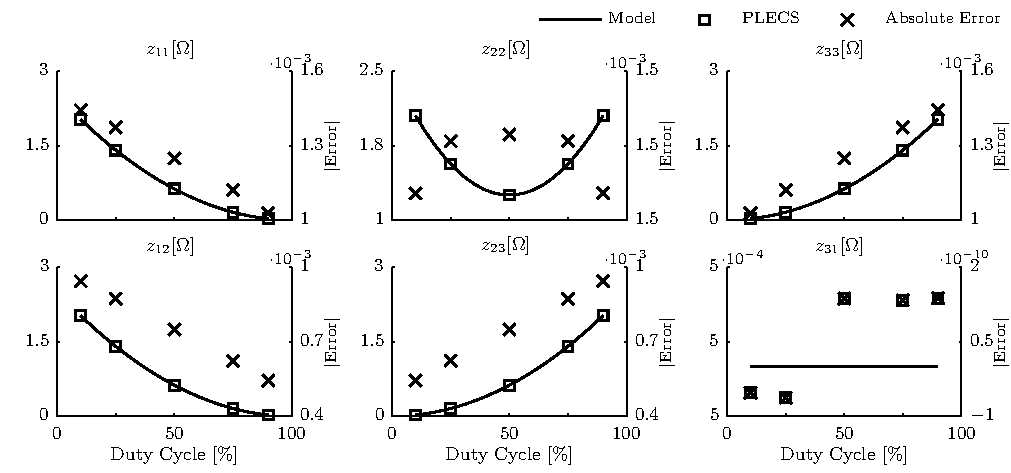
\includegraphics[page=1,width=12cm]{./4_model_validation/APEC_SIM_big}
  \centering
  \caption{SSL comparison between PLECS simulation and the proposed model.}
  \label{fig:sim_ssl}
\end{figure}


\begin{figure}[!h]
  \includegraphics[page=3,width=12cm]{./4_model_validation/APEC_SIM_big}
  \centering
  \caption{FSL comparison between PLECS simulation and the proposed model.}
  \label{fig:sim_fsl}
\end{figure}


\subsection{Experimental results}
An experimental set-up of the converter in was built. The converter uses four MOSFETs TN0104 from Supertex with typical \emph{on}-resistance of 1.5 $\Omega$. Two tantalum electrolytic capacitors of 10$\mu$F have been used as flying capacitors. The circuit was operated at 5kHz and the trans-resistance parameters are measured at different duty cycles. The results are compared with the model and  presented in Figure \ref{fig:meas_zscc}, it can be seen that the predictions match the measured values with less than 10\% error. All the trans-impedance values with the exception of  parameters $z_{31}$ and $z_{13}$ follow the trend with the duty cycle predicted by the model. $z_{31}$ and $z_{13}$ have a bigger error since these values are much smaller than the rest of the converter parameters and, therefore, more sensitive to the parasitics of the board.

\begin{figure}[!h]
\newcommand\pHeigh{2.750cm}
\newcommand\pWidth{2.500cm}
\centering
	\begin{subfigure}{\textwidth}
		\parbox[b]{0.3250\linewidth}{
		\centering
			\begin{tikzpicture}
    \pgfplotsset{
        width=\pWidth,
        height=\pHeigh,
        scale only axis,
        xlabel near ticks,
        ylabel near ticks,
        scaled y ticks= true ,
        enlarge x limits={0.1},
        enlarge y limits={0.1},
        every tick label/.append style={font=\footnotesize},
        }

	\begin{axis}[
		axis y line*=left,
		axis x line*=bottom,
		xticklabels={,,},
		ylabel = {$r_{scc} [\Omega]$},
		yticklabel style={text width=2.00em,align=right},
		title = {$z_{11}$},
		title style = {
    			font=\footnotesize },
    			at ={(0.75,0.75)},
		]

		\addplot[thin,black,smooth]
    		table [y=y1]{./4_model_validation/c10uF_bis/c10uF_bis_5kHz_Ymdl.dat};

		\addplot[semithick,mark=o,only marks]
    		table [y=y1]{./4_model_validation/c10uF_bis/c10uF_bis_5kHz_Ymeas.dat};

\end{axis}

\end{tikzpicture}

		}
		\parbox[b]{0.3250\linewidth}{
		\centering
			\begin{tikzpicture}
    \pgfplotsset{
        width=\pWidth,
        height=\pHeigh,
        scale only axis,
        xlabel near ticks,
        ylabel near ticks,
        scaled y ticks= true ,
        enlarge x limits={0.1},
        enlarge y limits={0.1},
        every tick label/.append style={font=\footnotesize},
        }

	\begin{axis}[
		axis y line*=left,
		axis x line*=bottom,
		xticklabels={,,},
		yticklabel style={text width=1.50em,align=right},
		title = {$z_{12}$},
		title style = {
    			font=\footnotesize },
    			at ={(0.75,0.75)},
		]

		\addplot[thin,black,smooth]
    		table [y=y4]{./4_model_validation/c10uF_bis/c10uF_bis_5kHz_Ymdl.dat};

		\addplot[semithick,mark=square,only marks]
    		table [y=y4]{./4_model_validation/c10uF_bis/c10uF_bis_5kHz_Ymeas.dat};

	\end{axis}

	\begin{axis}[
		axis y line*=right,
		axis x line=none,
		xticklabels={,,},
		yticklabel pos=right,
		yticklabel style={text width=1.50em,align=left,xshift=-0.50ex},
		enlarge y limits={0.15},
		]

		\addplot[semithick,mark=x,only marks]
    		table [y=y4]{./4_model_validation/c10uF_bis/c10uF_bis_5kHz_Yerr.dat};

	\end{axis}

\end{tikzpicture}

		}
		\parbox[b]{0.3250\linewidth}{
		\centering
			\begin{tikzpicture}
    \pgfplotsset{
        width=\pWidth,
        height=\pHeigh,
        scale only axis,
        xlabel near ticks,
        ylabel near ticks,
        scaled y ticks= true ,
        enlarge x limits={0.1},
        enlarge y limits={0.1},
        every tick label/.append style={font=\footnotesize},
        }

	\begin{axis}[
		axis y line*=left,
		axis x line*=bottom,
		xticklabels={,,},
		yticklabel style={text width=2.00em,align=right},
		title = {$z_{13}$},
		title style = {
    			font=\footnotesize },
    			at ={(0.75,0.75)},
		]

		\addplot[thin,black,smooth]
    		table [y=y7]{./4_model_validation/c10uF_bis/c10uF_bis_5kHz_Ymdl.dat};

		\addplot[semithick,mark=o,only marks]
    		table [y=y7]{./4_model_validation/c10uF_bis/c10uF_bis_5kHz_Ymeas.dat};

\end{axis}

\end{tikzpicture}

		}
	\end{subfigure}

	\begin{subfigure}{\textwidth}
		\parbox[b]{0.3250\linewidth}{
		\centering
			\begin{tikzpicture}
    \pgfplotsset{
        width=\pWidth,
        height=\pHeigh,
        scale only axis,
        xlabel near ticks,
        ylabel near ticks,
        scaled y ticks= true ,
        enlarge x limits={0.1},
        enlarge y limits={0.1},
        every tick label/.append style={font=\footnotesize},
        }

	\begin{axis}[
		axis y line*=left,
		axis x line*=bottom,
		xticklabels={,,},
		ylabel = {$r_{scc} [\Omega]$},
		yticklabel style={text width=1.50em,align=right},
		title = {$z_{21}$},
		title style = {
    			font=\footnotesize },
    			at ={(0.75,0.75)},
		]

		\addplot[thin,black,smooth]
    		table [y=y2]{./4_model_validation/c10uF_bis/c10uF_bis_5kHz_Ymdl.dat};

		\addplot[semithick,mark=square,only marks]
    		table [y=y2]{./4_model_validation/c10uF_bis/c10uF_bis_5kHz_Ymeas.dat};

	\end{axis}

	\begin{axis}[
		axis y line*=right,
		axis x line=none,
		xticklabels={,,},
		yticklabel pos=right,
		yticklabel style={text width=1.50em,align=left,xshift=-0.50ex},
		enlarge y limits={0.15},
		]

		\addplot[semithick,mark=x,only marks]
    		table [y=y2]{./4_model_validation/c10uF_bis/c10uF_bis_5kHz_Yerr.dat};

	\end{axis}

\end{tikzpicture}

		}
		\parbox[b]{0.3250\linewidth}{
		\centering
			\begin{tikzpicture}
    \pgfplotsset{
        width=\pWidth,
        height=\pHeigh,
        scale only axis,
        xlabel near ticks,
        ylabel near ticks,
        scaled y ticks= true ,
        enlarge x limits={0.1},
        enlarge y limits={0.1},
        every tick label/.append style={font=\footnotesize},
        }

	\begin{axis}[
		axis y line*=left,
		axis x line*=bottom,
		xticklabels={,,},
		yticklabel style={text width=2.00em,align=right},
		title = {$z_{22}$},
		title style = {
    			font=\footnotesize },
    			at ={(0.75,0.75)},
		]

		\addplot[thin,black,smooth]
    		table [y=y5]{./4_model_validation/c10uF_bis/c10uF_bis_5kHz_Ymdl.dat};

		\addplot[semithick,mark=o,only marks]
    		table [y=y5]{./4_model_validation/c10uF_bis/c10uF_bis_5kHz_Ymeas.dat};

\end{axis}

\end{tikzpicture}

		}
		\parbox[b]{0.3250\linewidth}{
		\centering
			\begin{tikzpicture}
    \pgfplotsset{
        width=\pWidth,
        height=\pHeigh,
        scale only axis,
        xlabel near ticks,
        ylabel near ticks,
        scaled y ticks= true ,
        enlarge x limits={0.1},
        enlarge y limits={0.1},
        every tick label/.append style={font=\footnotesize},
        }

	\begin{axis}[
		axis y line*=left,
		axis x line*=bottom,
		xticklabels={,,},
		yticklabel style={text width=1.50em,align=right},
		title = {$z_{23}$},
		title style = {
    			font=\footnotesize },
    			at ={(0.75,0.75)},
		]

		\addplot[thin,black,smooth]
    		table [y=y8]{./4_model_validation/c10uF_bis/c10uF_bis_5kHz_Ymdl.dat};

		\addplot[semithick,mark=square,only marks]
    		table [y=y8]{./4_model_validation/c10uF_bis/c10uF_bis_5kHz_Ymeas.dat};

	\end{axis}

	\begin{axis}[
		axis y line*=right,
		axis x line=none,
		xticklabels={,,},
		ylabel = {$\epsilon$},
		yticklabel pos=right,
		yticklabel style={text width=1.50em,align=left,xshift=-0.50ex},
		enlarge y limits={0.15},
		]

		\addplot[semithick,mark=x,only marks]
    		table [y=y8]{./4_model_validation/c10uF_bis/c10uF_bis_5kHz_Yerr.dat};

	\end{axis}

\end{tikzpicture}

		}
	\end{subfigure}

	\begin{subfigure}{\textwidth}
		\parbox[b]{0.3250\linewidth}{
		\centering
			\begin{tikzpicture}
    \pgfplotsset{
        width=\pWidth,
        height=\pHeigh,
        scale only axis,
        xlabel near ticks,
        ylabel near ticks,
        scaled y ticks= true ,
        enlarge x limits={0.1},
        enlarge y limits={0.1},
        every tick label/.append style={font=\footnotesize},
        }

	\begin{axis}[
		axis y line*=left,
		axis x line*=bottom,
		xlabel = {duty cycle},
		ylabel = {$r_{scc} [\Omega]$},
		yticklabel style={text width=1.50em,align=right},
		title = {$z_{31}$},
		title style = {
    			font=\footnotesize },
    			at ={(0.75,0.75)},
		]

		\addplot[thin,black,smooth]
    		table [y=y3]{./4_model_validation/c10uF_bis/c10uF_bis_5kHz_Ymdl.dat};

		\addplot[semithick,mark=square,only marks]
    		table [y=y3]{./4_model_validation/c10uF_bis/c10uF_bis_5kHz_Ymeas.dat};

	\end{axis}

	\begin{axis}[
		axis y line*=right,
		axis x line=none,
		yticklabel pos=right,
		yticklabel style={text width=1.50em,align=left,xshift=-0.50ex},
		enlarge y limits={0.15},
		]

		\addplot[semithick,mark=x,only marks]
    		table [y=y3]{./4_model_validation/c10uF_bis/c10uF_bis_5kHz_Yerr.dat};

	\end{axis}

\end{tikzpicture}

		}
		\parbox[b]{0.3250\linewidth}{
		\centering
			\begin{tikzpicture}
    \pgfplotsset{
        width=\pWidth,
        height=\pHeigh,
        scale only axis,
        xlabel near ticks,
        ylabel near ticks,
        scaled y ticks= true ,
        enlarge x limits={0.1},
        enlarge y limits={0.1},
        every tick label/.append style={font=\footnotesize},
        }

	\begin{axis}[
		axis y line*=left,
		axis x line*=bottom,
		xlabel = {duty cycle},
		yticklabel style={text width=1.50em,align=right},
		title = {$z_{32}$},
		title style = {
    			font=\footnotesize },
    			at ={(0.75,0.75)},
		]

		\addplot[thin,black,smooth]
    		table [y=y6]{./4_model_validation/c10uF_bis/c10uF_bis_5kHz_Ymdl.dat};

		\addplot[semithick,mark=square,only marks]
    		table [y=y6]{./4_model_validation/c10uF_bis/c10uF_bis_5kHz_Ymeas.dat};

	\end{axis}

	\begin{axis}[
		axis y line*=right,
		axis x line=none,
		yticklabel pos=right,
		yticklabel style={text width=1.50em,align=left,xshift=-0.50ex},
		enlarge y limits={0.15},
		]

		\addplot[semithick,mark=x,only marks]
    		table [y=y6]{./4_model_validation/c10uF_bis/c10uF_bis_5kHz_Yerr.dat};

	\end{axis}

\end{tikzpicture}

		}
		\parbox[b]{0.3250\linewidth}{
		\centering
			\begin{tikzpicture}
    \pgfplotsset{
        width=\pWidth,
        height=\pHeigh,
        scale only axis,
        xlabel near ticks,
        ylabel near ticks,
        scaled y ticks= true ,
        enlarge x limits={0.1},
        enlarge y limits={0.1},
        every tick label/.append style={font=\footnotesize},
        }

	\begin{axis}[
		axis y line*=left,
		axis x line*=bottom,
		xlabel = {duty cycle},
		yticklabel style={text width=2.00em,align=right},
		title = {$z_{33}$},
		title style = {
    			font=\footnotesize },
    			at ={(0.75,0.75)},
		]

		\addplot[thin,black,smooth]
    		table [y=y9]{./4_model_validation/c10uF_bis/c10uF_bis_5kHz_Ymdl.dat};

		\addplot[semithick,mark=o,only marks]
    		table [y=y9]{./4_model_validation/c10uF_bis/c10uF_bis_5kHz_Ymeas.dat};

\end{axis}

\end{tikzpicture}

		}
	\end{subfigure}

	\caption[Measured $\mathbf{Z_{scc}}$ from a 2:1 SCC experimental converter.]{Experimental results of the 2:1 SCC, with $f_{sw}=5kHz$. Comparison of the  measured (\emph{$\Box$ markers} ) trans-resistance parameters with the model predicted (\emph{solid line}), and the error ($\epsilon$) between the model and the measures (\emph{x markers}.)}
	\label{}
\end{figure}



\begin{figure}[!h]
\newcommand\pHeigh{2.750cm}
\newcommand\pWidth{2.500cm}
\centering
	\begin{subfigure}{\textwidth}
		\parbox[b]{0.3250\linewidth}{
		\centering
			\begin{tikzpicture}
    \pgfplotsset{
        width=\pWidth,
        height=\pHeigh,
        scale only axis,
        xlabel near ticks,
        ylabel near ticks,
        scaled y ticks= true ,
        enlarge x limits={0.1},
        enlarge y limits={0.1},
        every tick label/.append style={font=\footnotesize},
        }

	\begin{loglogaxis}[
		axis y line*=left,
		axis x line*=bottom,
		xticklabels={,,},
		ylabel = {$[\Omega]$},
		yticklabel style={text width=2.00em,align=right},
		title = {$z_{11}$},
		title style = {
    			font=\footnotesize },
    			at ={(0.75,0.75)},
		]

		\addplot[thin,black,smooth]
    		table [y=y1]{./4_model_validation/c10uF_bis_fsw/c10uF_bis_fsw_D=50_Ymdl.dat};

		\addplot[semithick,mark=square,only marks]
    		table [y=y1]{./4_model_validation/c10uF_bis_fsw/c10uF_bis_fsw_D=50_Ymeas.dat};

	\end{loglogaxis}

\end{tikzpicture}

		}
		\parbox[b]{0.3250\linewidth}{
		\centering
			\begin{tikzpicture}
    \pgfplotsset{
        width=\pWidth,
        height=\pHeigh,
        scale only axis,
        xlabel near ticks,
        ylabel near ticks,
        scaled y ticks= true ,
        enlarge x limits={0.1},
        enlarge y limits={0.1},
        every tick label/.append style={font=\footnotesize},
        }

	\begin{loglogaxis}[
		axis y line*=left,
		axis x line*=bottom,
		xticklabels={,,},
		yticklabel style={text width=2.00em,align=right},
		title = {$z_{12}$},
		title style = {
    			font=\footnotesize },
    			at ={(0.75,0.75)},
		]

		\addplot[thin,black,smooth]
    		table [y=y4]{./4_model_validation/c10uF_bis_fsw/c10uF_bis_fsw_D=50_Ymdl.dat};

		\addplot[semithick,mark=square,only marks]
    		table [y=y4]{./4_model_validation/c10uF_bis_fsw/c10uF_bis_fsw_D=50_Ymeas.dat};

	\end{loglogaxis}

\end{tikzpicture}

		}
		\parbox[b]{0.3250\linewidth}{
		\centering
			\begin{tikzpicture}
    \pgfplotsset{
        width=\pWidth,
        height=\pHeigh,
        scale only axis,
        xlabel near ticks,
        ylabel near ticks,
        scaled y ticks= true ,
        enlarge x limits={0.1},
        enlarge y limits={0.1},
        every tick label/.append style={font=\footnotesize},
        }

	\begin{loglogaxis}[
		axis y line*=left,
		axis x line*=bottom,
		xticklabels={,,},
		yticklabel style={text width=2.00em,align=right},
		title = {$z_{13}$},
		title style = {
    			font=\footnotesize },
    			at ={(0.75,0.75)},
		]

		\addplot[thin,black,smooth]
    		table [y=y7]{./4_model_validation/c10uF_bis_fsw/c10uF_bis_fsw_D=50_Ymdl.dat};

		\addplot[semithick,mark=square,only marks]
    		table [y=y7]{./4_model_validation/c10uF_bis_fsw/c10uF_bis_fsw_D=50_Ymeas.dat};

	\end{loglogaxis}

\end{tikzpicture}

		}
	\end{subfigure}

	\begin{subfigure}{\textwidth}
		\parbox[b]{0.3250\linewidth}{
		\centering
			\begin{tikzpicture}
    \pgfplotsset{
        width=\pWidth,
        height=\pHeigh,
        scale only axis,
        xlabel near ticks,
        ylabel near ticks,
        scaled y ticks= true ,
        enlarge x limits={0.1},
        enlarge y limits={0.1},
        every tick label/.append style={font=\footnotesize},
        }

	\begin{loglogaxis}[
		axis y line*=left,
		axis x line*=bottom,
		xticklabels={,,},
		ylabel = {$[\Omega]$},
		yticklabel style={text width=2.00em,align=right},
		title = {$z_{21}$},
		title style = {
    			font=\footnotesize },
    			at ={(0.75,0.75)},
		]

		\addplot[thin,black,smooth]
    		table [y=y2]{./4_model_validation/c10uF_bis_fsw/c10uF_bis_fsw_D=50_Ymdl.dat};

		\addplot[semithick,mark=square,only marks]
    		table [y=y2]{./4_model_validation/c10uF_bis_fsw/c10uF_bis_fsw_D=50_Ymeas.dat};

	\end{loglogaxis}

\end{tikzpicture}

		}
		\parbox[b]{0.3250\linewidth}{
		\centering
			\begin{tikzpicture}
    \pgfplotsset{
        width=\pWidth,
        height=\pHeigh,
        scale only axis,
        xlabel near ticks,
        ylabel near ticks,
        scaled y ticks= true ,
        enlarge x limits={0.1},
        enlarge y limits={0.1},
        every tick label/.append style={font=\footnotesize},
        }

	\begin{loglogaxis}[
		axis y line*=left,
		axis x line*=bottom,
		xticklabels={,,},
		yticklabel style={text width=2.00em,align=right},
		title = {$z_{22}$},
		title style = {
    			font=\footnotesize },
    			at ={(0.75,0.75)},
		]

		\addplot[thin,black,smooth]
    		table [y=y5]{./4_model_validation/c10uF_bis_fsw/c10uF_bis_fsw_D=50_Ymdl.dat};

		\addplot[semithick,mark=square,only marks]
    		table [y=y5]{./4_model_validation/c10uF_bis_fsw/c10uF_bis_fsw_D=50_Ymeas.dat};

	\end{loglogaxis}

\end{tikzpicture}

		}
		\parbox[b]{0.3250\linewidth}{
		\centering
			\begin{tikzpicture}
    \pgfplotsset{
        width=\pWidth,
        height=\pHeigh,
        scale only axis,
        xlabel near ticks,
        ylabel near ticks,
        scaled y ticks= true ,
        enlarge x limits={0.1},
        enlarge y limits={0.1},
        every tick label/.append style={font=\footnotesize},
        }

	\begin{loglogaxis}[
		axis y line*=left,
		axis x line*=bottom,
		xticklabels={,,},
		yticklabel style={text width=2.00em,align=right},
		title = {$z_{23}$},
		title style = {
    			font=\footnotesize },
    			at ={(0.75,0.75)},
		]

		\addplot[thin,black,smooth]
    		table [y=y8]{./4_model_validation/c10uF_bis_fsw/c10uF_bis_fsw_D=50_Ymdl.dat};

		\addplot[semithick,mark=square,only marks]
    		table [y=y8]{./4_model_validation/c10uF_bis_fsw/c10uF_bis_fsw_D=50_Ymeas.dat};

	\end{loglogaxis}

\end{tikzpicture}

		}
	\end{subfigure}

	\begin{subfigure}{\textwidth}
		\parbox[b]{0.3250\linewidth}{
		\centering
			\begin{tikzpicture}
    \pgfplotsset{
        width=\pWidth,
        height=\pHeigh,
        scale only axis,
        xlabel near ticks,
        ylabel near ticks,
        scaled y ticks= true ,
        enlarge x limits={0.1},
        enlarge y limits={0.1},
        every tick label/.append style={font=\footnotesize},
        }

	\begin{loglogaxis}[
		axis y line*=left,
		axis x line*=bottom,
		xlabel = {$f_{sw}$},
		ylabel = {$[\Omega]$},
		yticklabel style={text width=2.00em,align=right},
		title = {$z_{31}$},
		title style = {
    			font=\footnotesize },
    			at ={(0.75,0.75)},
		]

		\addplot[thin,black,smooth]
    		table [y=y3]{./4_model_validation/c10uF_bis_fsw/c10uF_bis_fsw_D=50_Ymdl.dat};

		\addplot[semithick,mark=square,only marks]
    		table [y=y3]{./4_model_validation/c10uF_bis_fsw/c10uF_bis_fsw_D=50_Ymeas.dat};

	\end{loglogaxis}

\end{tikzpicture}

		}
		\parbox[b]{0.3250\linewidth}{
		\centering
			\begin{tikzpicture}
    \pgfplotsset{
        width=\pWidth,
        height=\pHeigh,
        scale only axis,
        xlabel near ticks,
        ylabel near ticks,
        scaled y ticks= true ,
        enlarge x limits={0.1},
        enlarge y limits={0.1},
        every tick label/.append style={font=\footnotesize},
        }

	\begin{loglogaxis}[
		axis y line*=left,
		axis x line*=bottom,
		xlabel = {$f_{sw}$},
		yticklabel style={text width=2.00em,align=right},
		title = {$z_{32}$},
		title style = {
    			font=\footnotesize },
    			at ={(0.75,0.75)},
		]

		\addplot[thin,black,smooth]
    		table [y=y6]{./4_model_validation/c10uF_bis_fsw/c10uF_bis_fsw_D=50_Ymdl.dat};

		\addplot[semithick,mark=square,only marks]
    		table [y=y6]{./4_model_validation/c10uF_bis_fsw/c10uF_bis_fsw_D=50_Ymeas.dat};

	\end{loglogaxis}

\end{tikzpicture}

		}
		\parbox[b]{0.3250\linewidth}{
		\centering
			\begin{tikzpicture}
    \pgfplotsset{
        width=\pWidth,
        height=\pHeigh,
        scale only axis,
        xlabel near ticks,
        ylabel near ticks,
        scaled y ticks= true ,
        enlarge x limits={0.1},
        enlarge y limits={0.1},
        every tick label/.append style={font=\footnotesize},
        }

	\begin{loglogaxis}[
		axis y line*=left,
		axis x line*=bottom,
		xlabel = {$f_{sw}$},
		yticklabel style={text width=2.00em,align=right},
		title = {$z_{33}$},
		title style = {
    			font=\footnotesize },
    			at ={(0.75,0.75)},
		]

		\addplot[thin,black,smooth]
    		table [y=y9]{./4_model_validation/c10uF_bis_fsw/c10uF_bis_fsw_D=50_Ymdl.dat};

		\addplot[semithick,mark=square,only marks]
    		table [y=y9]{./4_model_validation/c10uF_bis_fsw/c10uF_bis_fsw_D=50_Ymeas.dat};

	\end{loglogaxis}

\end{tikzpicture}

		}
	\end{subfigure}

	\caption[Measured $\mathbf{Z_{scc}}$ from a 2:1 SCC experimental converter.]{Experimental results of the 2:1 SCC, with $f_{sw}=50Hz$. Comparison of the  measured (\emph{$\Box$ markers} ) trans-resistance parameters with the model predicted (\emph{solid line}), and the error ($\epsilon$) between the model and the measures (\emph{x markers}.)}
	\label{}
\end{figure}



%The measured results of the experimental set-up can be improved mounting the circuit in a PCB with less parasitics and operated at higher switching frequencies by using ceramic capacitors instead of the tantalum ones .
\section{Summary}
The presented model is a valuable tool for  modeling a broad range of SCCs, from the classical approach of a single output converter to the new architectures where SCCs are combined with inductors. Unlike the previous models, this method allows to model the behaviour of multiple current loaded outputs, including their coupling relations. The model has been verified with simulations and experiments, and for both cases compares favorably. Since the resulting model is based on analytical expressions; the computation time is dramatically faster than any time-domain based simulator.

At the same time, it has been demonstrated that the original charge flow method was inaccurate in the SSL region, specially when the output capacitor was comparable in size to the flying capacitors. And it was not sensible to the variations of the duty cycle, leading to the wrong estimation of the output resistance of the converter.

The results presented the best accuracy of the model when the converter operates close to the well-defined switching limits, SSL and FSL, with relative errors below $5\%$. When the converter operates in region between the two limits, the relative error can increase up to $20\%$, since the value is approximated from the two asymptotical limits. With regard to the different proposed approximations, results shown the best accuracy using the first proposed approximation of $r_{scc} = \sqrt{r_{ssl}^2 + r_{fsl}^2}$.

\clearpage
\bibliographystyle{plainnat}
\bibliography{references} 
%%\part[SCC for LED drivers]{Switched Capacitor Converters for LED drivers}
\label{ch:h_scc}

\chapter{}
Switched Capacitor Converters (SCCs) are \emph{dc-dc} power circuits composed only by switches and capacitors that provide efficient voltage conversion. SCCs have been long known and utilized, initially for voltage multiplication and more recently for voltage regulation as well. Compared to inductor based power converters, the absence of magnetic elements makes them suitable for high density power systems and integrated solutions, such as Power-System-in-Package (PSiP) or Power-System-on-Chip (PSoC). 

The power conversion capabilities and the favorable characteristics for integration combined with the growing necessities for integration in the LED driver circuits was the initial motivation of the presented work. This first chapter will make the reader to understand the operation of the converter, the context of the general applications of SCC and the specific work done related to LED driving.

\section{Operation of Switched Capacitor Converters}

A Switched Capacitor Converter is a electronic circuit only composed by interconnected capacitors and switches that produces voltage-to-voltage conversion. The converter has two o more configuration modes, referred as phases, that sequentially change in order to achieve power conversion. 

\begin{figure}[!h]

\centering
\ctikzset { bipoles/length=1cm}
%\ctikzset { scale=0.5}
    \begin{subfigure}[t]{\textwidth}
    %\floatbox[{\capbeside\thisfloatsetup{capbesideposition={left,top},capbesidewidth=1cm}}]{figure}[\FBwidth]
%{\caption{A test figure with its caption side by side}\label{fig:test}}{
    \centering
    %\ctikzset { bipoles/length=1cm}
        \begin{circuitikz}[american voltages,scale=0.6]
        %\draw (0,11) node[anchor=north]{ };
        \draw
                %Input Supply
                (0,0)  to[V=$v_{i}$]
                %Draw Switches
                (0,10)  --
                (5,10)  to[switch=$s_1$] %S1
                (5,8)   to[switch=$s_2$] %S2
                (5,6)   to[switch=$s_3$] %S3
                (5,4) --
                %left branch
                (3,4)   to[switch=$s_5$]
                (3,2)   to[switch=$s_4$]
                (3,0);

        \draw   %right branch
                (5,4) --
                (7,4)   to[switch=$s_6$]
                (7,2)   to[switch=$s_7$]
                (7,0) -- (0,0);

        \draw %Capacitor C1
               (3,2) -- (2,2) -- (2,4)
                to[pC=$c_1$] (2,8) --
               (5,8);



        \draw %Capacitor C2
                (7,2) -- (8.25,2) --
               (8.25,4) to[pC=$c_2$](8.25,6) --
               (5,6);

        \draw %Capacitor C3
               (5,0) to[pC=$c_3$]
               (5,4);
               
         \draw (7,4) to[short,-o] (10,4) node[anchor=west] {$v_o$};
         \draw (7,0) to[short,-o] (10,0) node[anchor=west] {};
         \draw (10,4) to[open,v^=$v_{out}$] (10,0);

         \end{circuitikz}
     \subcaption{Circuit diagram the two phase 3:1 Dickson Converter.}
     \label{fig:demo_full_sch}
    \end{subfigure}

    \begin{subfigure}[t]{\textwidth}
    \centering
    %\ctikzset { bipoles/length=1cm}
        \begin{circuitikz}[american voltages,scale=0.6]
        \draw (-1,7) node[anchor=north]{ };
        \draw
                %Input Supply
                (-1,0)  to[V=$v_{i}$]
                %Draw Switches
                (-1,6)  --
                (4,6);
                
        %Capacitor C1
        \draw   (4,3) to[pC=$c_1$] (4,6);
        
        %Capacitor C2
        \draw (2,0)to[pC=$c_2$](2,3) --(4,3);
        
        %Capacitor C3
        \draw  (-1,0)--
               (6,0) to[pC=$c_3$]
               (6,3) -- (4,3);

         \draw (6,3) to[short,-o] (7.5,3) node[anchor=west] {$v_o$};
         \draw (6,0) to[short,-o] (7.5,0) node[anchor=west] {};
         \draw (7.5,3) to[open,v^=$v_{out}$] (7.5,0);
         \end{circuitikz}
     \subcaption{First phase, odd switched are closed and even switches are open.}
     \label{fig:demo_full_p1}
     \end{subfigure}

     \begin{subfigure}[t]{\textwidth}
      \centering
      \begin{circuitikz}[american voltages,scale=0.6]
        \draw (0,7) node[anchor=north]{ };
        \draw   %Input Supply
                (-1,0)  to[V=$v_{i}$]
                %Draw Switches
                (-1,6);

        \draw   (5,3) to[pC=$c_2$] (5,6);

        \draw %Capacitor C1
               (2,0)to[pC=$c_1$](2,6) --(5,6);

        \draw %Capacitor C3
               (5,0) to[pC=$c_3$]
               (5,3) -- (5,3);

         \draw (5,3) to[short,-o] (7.5,3) node[anchor=west] {$v_o$};
         \draw (-1,0) to[short,-o] (7.5,0) node[anchor=west] {};
         \draw (7.5,3) to[open,v^=$v_{out}$] (7.5,0);
         
         %\draw ()
         \end{circuitikz}
     \subcaption{Second phase, even switched are closed and odd switches are open.}
     \label{fig:emo_full_p2}
     \end{subfigure}
\caption{}
\label{fig:emo_full}
\end{figure}


\section[Chronological Vision of SCC]{A chronological vision of Switched Capacitor Converters}

The first Switched Capacitor Circuit was proposed in 1919 by Heinrich Greinacher. The \emph{Voltage Multiplier Rectifier}
multiplied the peak voltage of an AC supply to a DC voltage proportional to the number of stages. In 1932 J.D. Cockcroft and E.T.S. Walton used this circuit to generate very high voltage potentials,up to 800 kilovolts, for their particle accelerator ~\cite{30Cockcroft}; the picture of Figure~\ref{fig:Cockcroft_VMR} shows one of the used voltage multipliers. Subsequently, this circuit become widely used in television sets to supply high voltage to the cathode ray tube ~\cite{70Buechel} and later it was used in space applications~\cite{86Weinberg}. D.L. Waidelich and J.S. Brugler made some contributions to determine equivalent series resistance~\cite{44Waidelich,71Brugler} and Brugler and L. Chua proposed a unified approach to generate and analyse new topologies
~\cite{71Brugler,77Lin}.

\begin{figure}[!h]
\centering
 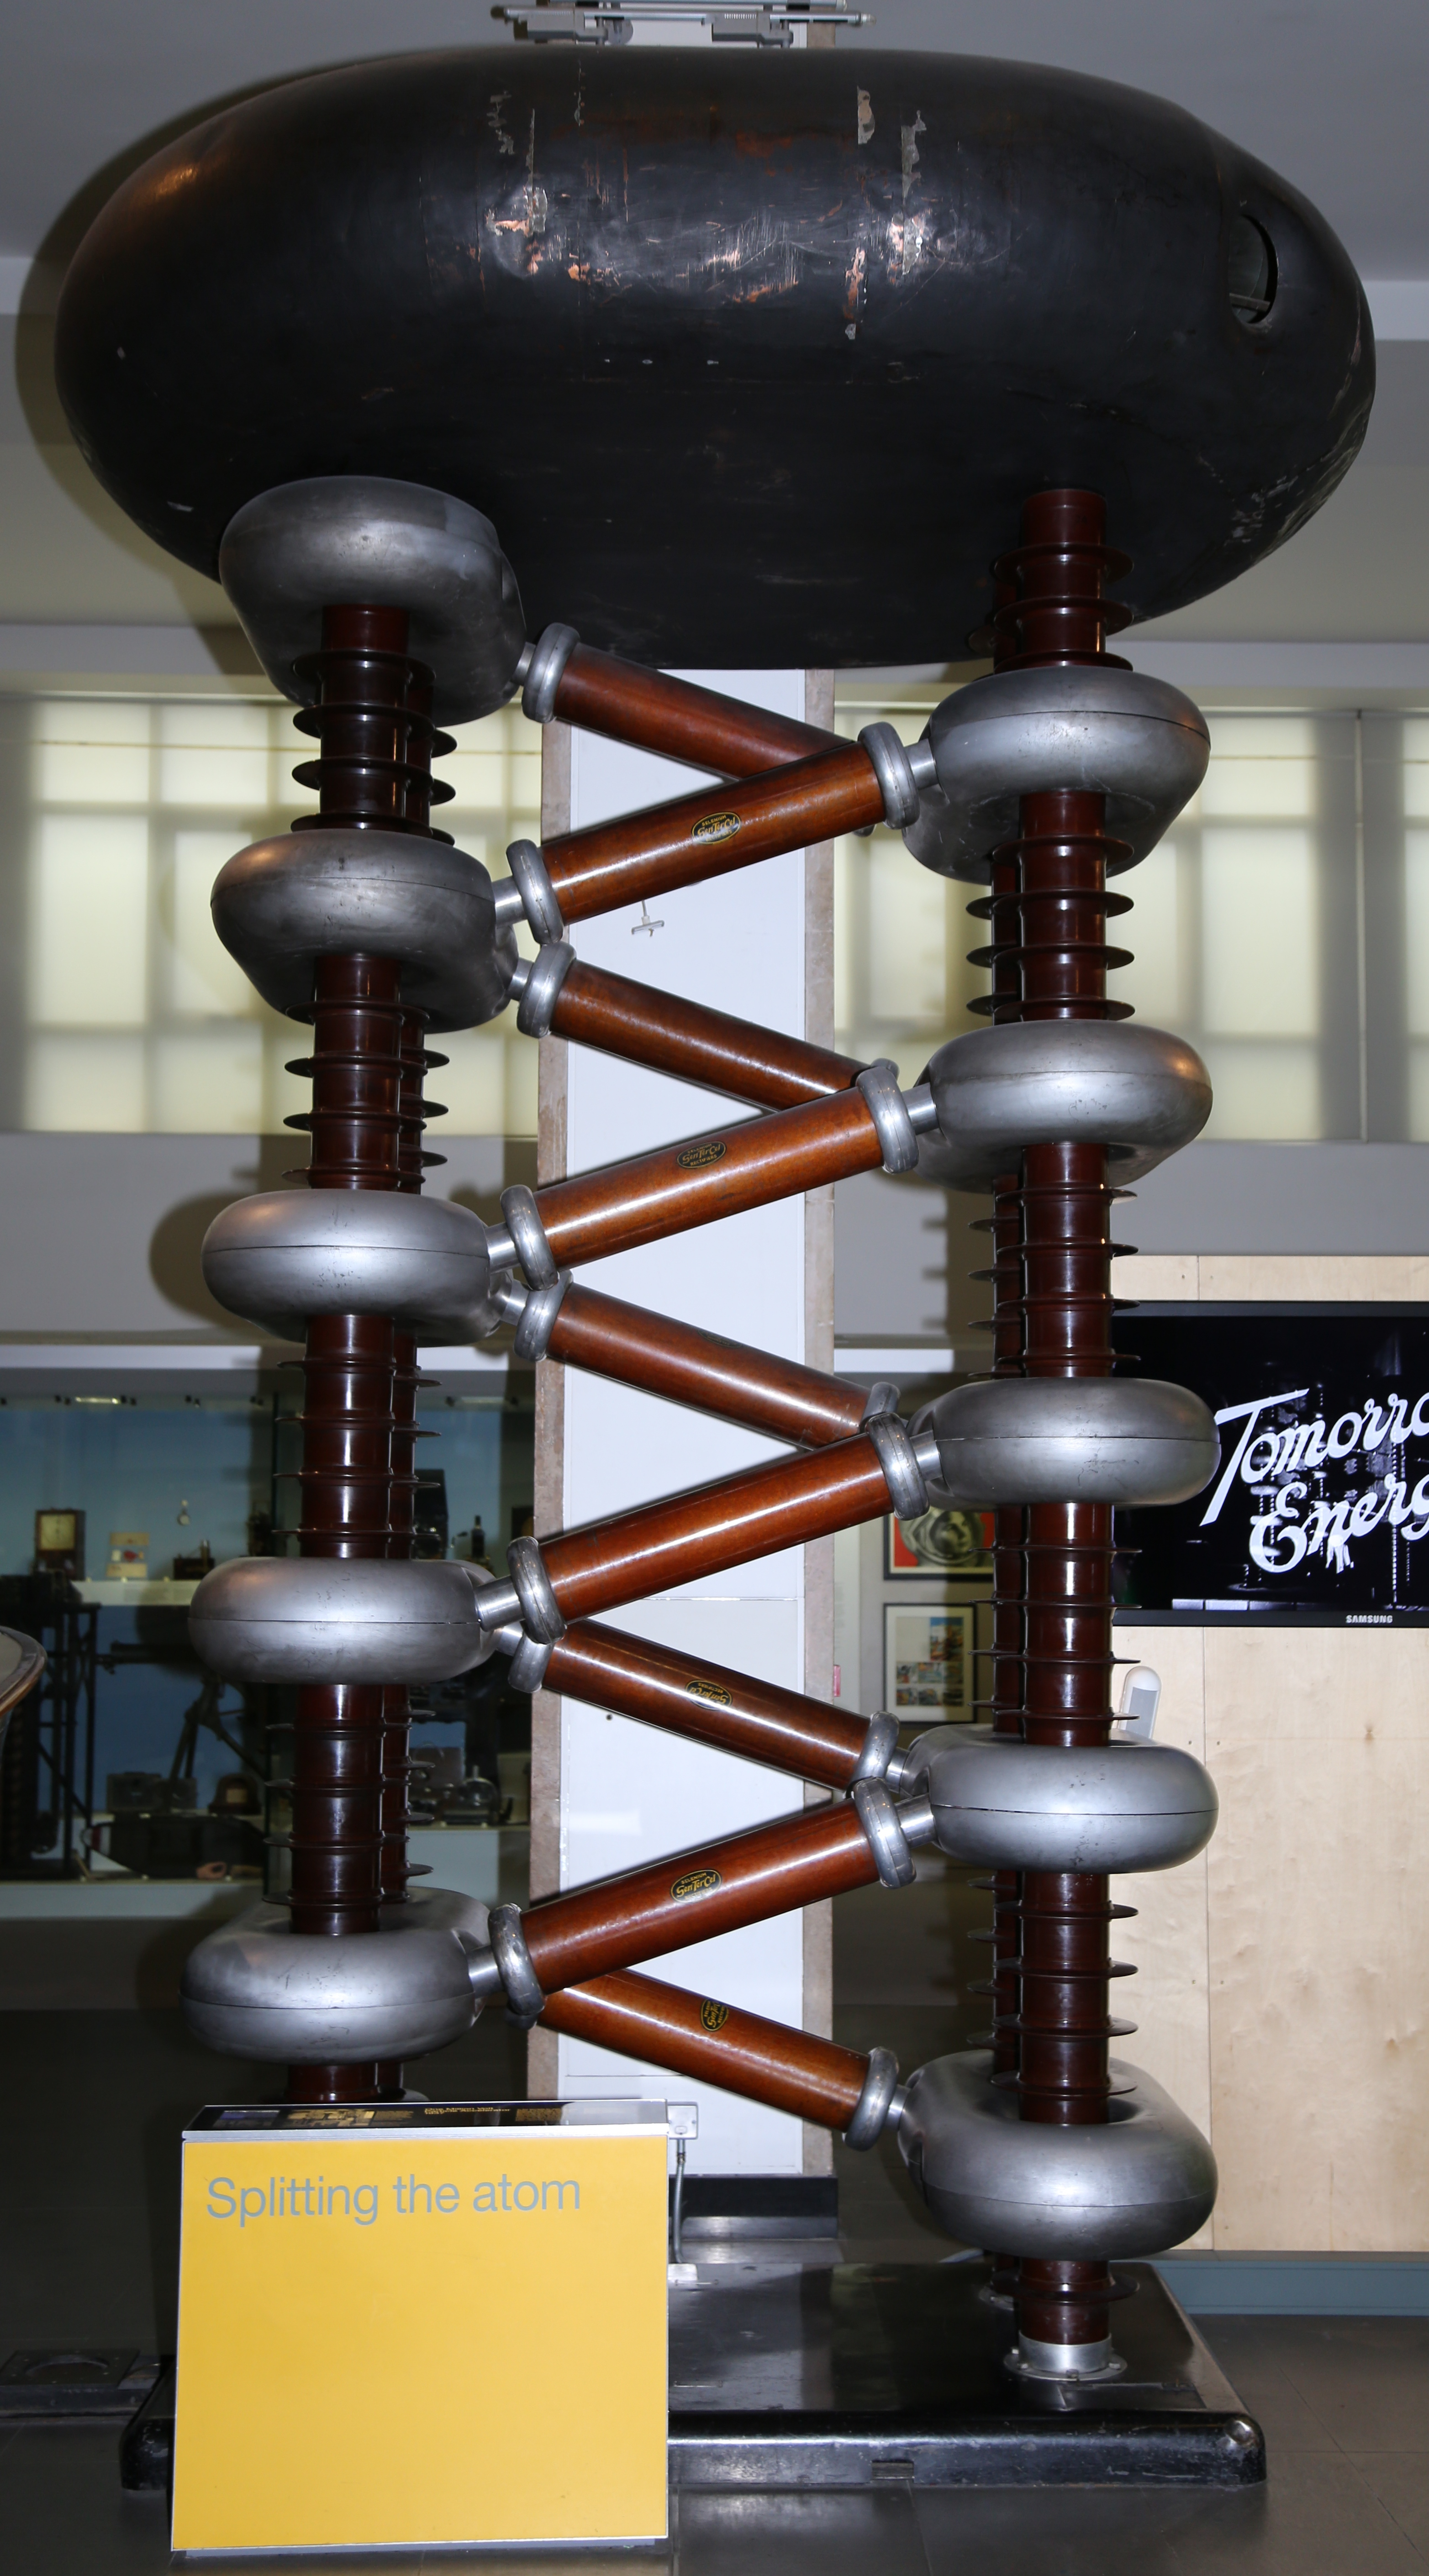
\includegraphics[width=6cm]{./1_modeling/img/CockcroftWaltonGenerator.jpg}
%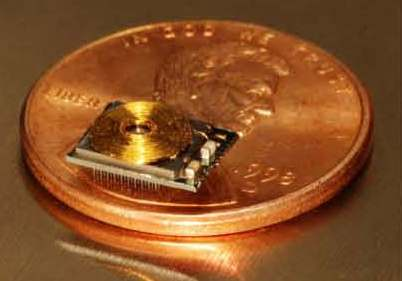
\includegraphics[width=6cm]{./0_intro/img/FSolzbacher01.jpg}
\caption{Cockcroft-Walton voltage multiplier built in 1937 by \emph{Philips Research Labs} in Eindhoven, now exposed in the \emph{Natural Science Museum} of London\\
\emph{Source:"Cockcroft–Walton generator 2012" by Geni. Licensed under GFDL via Wikimedia Commons  %http://commons.wikimedia.org/wiki/File:Cockcroft%E2%80%93Walton_generator_2012.JPG#/media/File:Cockcroft%E2%80%93Walton_generator_2012.JPG
}}
\label{fig:Cockcroft_VMR}
\end{figure}


In 1976, J.F. Dickson ~\cite{76Dickson} introduced a modification of the Cockcroft-Walton circuit to enable the integration of a voltage multiplier in an MNOS non volatile memory IC. The so-called Dickson charge-pump boosted the DC supply voltage proportionally to the number of stages in the pump. At same time, the new circuit mitigated the effects of the integrated capacitor stray capacitances on the voltage gain and reduced the output impedance of the converter increasing the current throughput. After the Dickson charge-pump other topologies~\cite{09Seeman} have been reported, such as the series-parallel converter ~\cite{94Ngo,94Cheong}, which allowed rational conversion ratios. F. Ueno \textit{et al.} ~\cite{91Ueno} presented yet another topology with conversion ratios corresponding to Fibonacci series,$k=1,2,3,5,8,..$ ,achieving higher conversion ratios using fewer capacitors ~\cite{95Makowski,09Allasasmeh}.  F.L. Luo  ~\cite{02Luo} proposed a topology cascading voltage doublers cells where the conversion ratio follows a quadratic relationship with the number of cells, and J. A. Starzyk ~\cite{01Starzyk} reviewed the same concept with a multi-phase topology that can achieve the same gain with fewer capacitors.



Two important concepts have been introduced to SC converters in order to reduce the current ripples and conduced Electromagnetic Interferences (EMI):
\begin{description}
  \item[Interleaving] also improves the efficiency since the it can reduce the value for the output capacitor. There are different reported implementations of 2-phase ~\cite{07Chang,99Chung}, 16-phase ~\cite{09Breussegem,14Andersen}, 32-phase~\cite{10Le} 64-phase~\cite{15Andersen}.
  \item[Current Mode] Charge-Pumps ~\cite{96Zhu,09Das} where the process of charge or discharge -or both- are controlled with a current source.
\end{description}

There are other innovative approaches where SCCs are combined with inductor based converters, also referred as \emph{hybrid} SCCs. The combination of both achieve large conversion ratios with tighter regulation. There are a large number of hybrid solutions where a SC cell is integrated into an inductor based converter ~\cite{05Axelrod,08Axelrod, 11Mayo,11Miranda,12Kline}. Lately, a couple of papers ~\cite{12Zhigang,11Dazhong} presented a Maximum Power Point Tracking (MPPT) converter for Photovoltaic (PV) cells employing a SC converter in parallel with an inductor based converter. This hybrid combinations offer another family of converters known as \emph{Resonant Switched Capacitor Converters} (RSCC), where the capacitors are charged through resonant transitions, thus eliminating the capacitor charge transfer losses.  K.W.E. Cheng ~\cite{01Cheng} in 2001 presented an early  work where in the topic using inductors limit the currents thought the capacitors and charging and discharging the capacitors with resonant transitions.  Subsequently, many publications appeared ~\cite{05Lee,10Cao,11Gebben,07Shoyama} presenting applications and uses of this converter family. Initial RSCC topologies made use of multiple inductors to guarantee a resonant transition for all capacitors, recent works~\cite{13Kesarwani,13Schaef,14Kesarwani,15Schaef} presented new topologies that reduced the number of inductors to achieve these resonant transitions.


\section{Sate of the Art of Switched Capacitor LED drivers}

One of the most popular application of SCCs is indeed as LED drivers for portable devices. Low power White LEDs (W-LEDs) are widely applied for back-lighting Liquid Crystal Display (LCD) in devices such as laptops, mobile phones and tablets. These applications require to generate a voltage above the LED forward voltage ($v_f$) from the battery, what can not been achieved with just using a linear drivers since the battery voltage is easily below to $v_f$  as it discharges. Normally theses drivers implement step-up or step-down to convert the battery right above the $v_f$.

\begin{figure}[t]
    \centering
    \begin{circuitikz} [scale=0.65]
    \ctikzset{bipoles/length=0.85cm}
   \draw[thick] (2.5,0.25) --
                (2.5,6.5) --
                (11.5,6.5) --
                (11.5,0.25) --
                (2.5,0.25);

    %Draw SCC block with capacitors
    \draw (3,1) --
          (3,6) --
          (5,6) --
          (5,1) --
          (3,1);

    \draw (4,1.25) node[rotate=90,anchor=west] {\emph{Multi-ratio SCC}};

    \draw (3,2) --
          (1.5,2) to[capacitor]
          (1.5,3) --
          (3,3);

    \draw (3,4) --
          (1.5,4) to[capacitor]
          (1.5,5) --
          (3,5);

    \draw (5,5.5) to[short,-o] (14,5.5);
    \draw (13,5.5) to[capacitor] (13,4.5) node[sground]{};

    \draw (4,1) -- (4,0) node[sground,scale=0.75]{};

   %Draw linear drivers
   \draw  (4,0.5) -- (10.5,0.5) -- (10.5,1);

   %First transitor
   \draw   (10,1) -- (10,1.5) node[npn,anchor=E,scale=0.5](npn1){}
           (npn1.C) -- (10,2.75) to[short,-o] (12,2.75);

   %Second transitor
   \draw  (10,1) -- (11,1)
           node[npn,anchor=E,scale=0.5](npn2){}
           (npn2.C) -- (11,2.25) to[short,-o] (12,2.25);

   %Controller box
   \draw (5.5,1) -- (8.5,1) -- (8.5,3) -- (5.5,3) -- (5.5,1);
   \draw (5.75,2) node[anchor=west, text width = 1.75cm]{Intensity Controller};
   \draw (npn2.B) -| (8.5,2);
   \draw (npn1.B) -| (8.5,2);

   %LEDs

   \draw [dashed] (14.25,5.5) to[short,o-] (15,5.5)
                    to[leD*] (15,2.75) to[short,-o] (12.25,2.75);

   \draw [dashed] (15,5.5) -- (17,5.5)
                    to[leD*] (17,2.25) to[short,-o] (12.25,2.25);

   %Add battery

   \draw (-1,0) node[sground,scale=0.75]{};
   \draw (-1,0) to[battery] (-1,6)
         -- (2.5,6);

    \end{circuitikz}
    \caption{Block diagram of a generic driver for backlighting applications.}
    \label{fig:backlight_LED}
\end{figure}

There is a large portfolio of available ICs, designated as Charge-Pumps (CPs), for driving LEDs in portable devices. Some commercial products are for instance  the \emph{MAX88779} \footnote{Maxim\textsuperscript{\textregistered} Charge Pump for Backlight/Flash/RGB LEDs with Safety Timer } or the \emph{MCP1252/3} \footnote{Microchip\textsuperscript{\textregistered} Low noise, Positive-Regulated Charge Pump}. These circuits  can drive withe, RGB or Flash LEDs from a Lithium-Ion battery only by adding a few external capacitors capacitors.  Generally these chips integrate an multi-target SCC with different conversion ratios (1:1, 3:2, 2:1) along with a series current regulator for each LED channel a shown in the block diagram of Figure~\ref{fig:backlight_LED}. Various publications ~\cite{07Feng,09Wu,10Yin} proposed enhancements in the architectures in order to reduce the parasitic losses bringing the efficiency close to the theoretical limit. Such drivers are used in applications below a 1$W$ and currents below hundred $mA$, their efficiency derates as the LED voltage moves away from the target voltage.

Besides the backlighting ICs, there are no other commercial LED drivers based on SCC. However that topic has been present in several research publications for the last years with few interesting publications targeting mains connected drivers. In 2008, K.H. Lee \emph{et al.}~\cite{08Lee} presented a SC step-down converter composed of several cascaded Series-Parallel that supplied from rectified 220$V_{rms}$ an LED string of 75V at 15W. In the proposed solution the LEDs are directly supplied using flying capacitors what produces pulsating currents in the string and its average values is controlled modulating the frequency of the converter. The cascaded topology minimized the number of components, switched and capacitors, for the required conversion ration (fixed by the LED string).

In 2012, M. Kline \emph{et al.} ~\cite{12Kline} proposed a isolated \emph{DC}/\emph{DC} converter that combined a SCC stage with series-LC resonant converter.  The SCC stage decreased  the rectified mains voltage, reducing the voltage stress in switches, capacitors and the elements of the resonant tank. The lower voltage stress allows a reduction in the volume of the passive components and the total area in the silicone. By controlling the frequency and the duty cycle of the SCC stage current through the LEDs can be regulated, resulting in a very efficient solution. In a recent publication they presented an implementation where power train and control where integrated in different stackable ICs modules~\cite{13Kline}.

The different applications show an increasing interest in using SCC for LED drivers. It is evident that the approach used in portable devices can no be further extended in for high powers and higher voltages. The use of a bear SCC can never satisfy the requirements of LED drivers due to the following facts:
\begin{itemize}
  \item Only provide voltage-to-voltage conversion
  \item Fixed conversion ratios
  \item Regulation is provided by series shunting
\end{itemize}
These limitations combined with the abrupt characteristics I-V of the LEDs makes barely impossible to provide high efficient solutions with the single use of SCC. The converters would require to have a large number of conversion ratios with a very large granularity to avoid uncontrolled currents flowing through the LEDs.

The research presented in this work aims to explore the possibilities of the SCC for LED drivers and the conducting path is based in the combination of the with inductors. The overall solution improves the power density and reduced form factor of the present solutions.



\section*{Power Levels and Integration}

There are not intrinsic implications that limit the output power of a Switched Capacitor converter, but the boundary conditions. There are implementations ranging from tens of milliwatts to tens of kilowatts, where the difference only relies in the used technology. They can be classified in 3 groups: Fully integrated circuits, integrated circuits with external capacitors and discrete solutions.

Full integrated converter are suitable for very lower power applications from some microwatts up to some tens of milliwatts. These solutions are implemented in standard processes (CMOS, BiCMOS or Bipolar) where the priority is in achieve an integrated solution rather than efficient. These converters have very poor efficiency up to 60\%, due to the low energy density and poor quality of the capacitors available in those processes. The second group overcomes this problem using external capacitors. These converters integrate the control and the power train in a single chip with a stadard CMOS process, offering  output power up to one watt and peak efficiencies of 95\%. In this case, the CMOS switches limit the converter efficiency and scalavility in power.
The implementations with discrete components enable output powers up to kilowatts with peak efficiencies above 95\%. Discrete semiconductor switches can offer lower channel resitance and better switching characterisitcs, reducing ohmic resitance and enabeling higher switching frequencies.  \emph{ \color{red} Silicon power MOSFET are the dominant in discrete implementations, but recent publications used Galiun-Nitride HEMT switches ~\cite{11Scott,12Scott}}.

The limiting factor of the output power of a SC converter is driven by the boundary conditions of the technology. Up to now, integrated SC converters designs have been covered addressing the problem with the standard process in VLSI, in order to have compact power conversion units at the lowest cost. The current technologies can easily improve the present solutions, for instance, a Power-System on Package (PSoC) integrating switches and capacitors would already reduce the series resistance of the pins and optimize the silicon die area of the present integrated converters with external capacitors. The current technologies offer the possibility to achieve integrated SC converters processing higher powers, but it would require to combine them in non-standard processes.

\emph{\color{red} Missing refs!}


%\bibliographystyle{plainnat}
%\bibliography{phd_bib} 


%\bibliographystyle{numerical}
%\bibliography{phd_bib}

%

\chapter[Advanced Modeling of SCC]{Advanced Modeling of Switched Capacitor Converters}

\section{Introduction}

\section{Single Output Converters}
Switched Capacitor Converters (SCCs) are considered to be a two-port converter with single input and a single output as shown in Fig.\ref{fig:two_port}. The input port is connected to a voltage source and the output port feeds the load. The SCC provides between input, $v_i$, and output, $v_o$, a voltage conversion, $m$,  that  steps up, steps down or/and inverts the polarity of the input voltage. Up to present all the circuit theory devoted SCCs is valid only for the two-port configuration, therefore this section is dedicated to revisit the classical concepts of single output SCC and to introduce new ones that enable a broader use of such converters.

\begin{figure}[!h]
\centering
\ctikzset { bipoles/length=1cm}
\begin{circuitikz}[scale=0.65]
\draw
    (1,0) to[short,o-]
    (0,0) to[V = $V_{supply}$]
    (0,3) to[short,-o]
    (1,3) ;

\draw
    (2,3) --
    (2.5,3)

    (2,0) --
    (2.5,0)

    node[ocirc]  (IC)  at (2,0) {}
    node[ocirc]  (I) at (2,3) {}
    (I) to[open,v=$v_{i}$] (IC);


\draw [thick]
    (2.5,-0.5) --
    (2.5,3.5)  --
    (5.5,3.5)  --
    (5.5,-0.5) --
    (2.5,-0.5);

\draw (4,2)node[anchor=north]{$\frac{v_o}{v_{i}}=m$} ;
\draw
    (5.5,3) -- (6,3)
    (5.5,0) -- (6,0)
    node[ocirc]  (O)  at (6,3) {}
    node[ocirc]  (OC) at (6,0) {}
    (O) to[open,v^<=$v_{o}$] (OC);

\draw
    (7,0) to[short,o-]
    (8,0) to[ R= $Load$,mirror]
    (8,3) to[short,-o]
    (7,3) ;
\end{circuitikz}
\label{fig:two_port}
\caption{General two port configuration of a Switched Capacitor Converter. }
\end{figure}


\subsection[Introducing H-SCC]{The Hybrid-SCC: Identifying Outputs in Switched Capacitor Converters}

Two types of nodes can be identified in a Switched Capacitor Converter, as shown in Fig. \ref{fig:dc_pwm_nodes}:
\begin{itemize}
  \item Fixed voltage \emph{dc}-nodes, node $a$ % node $a$ in Fig. \ref{fig:dc_pwm_nodes}
  \item Floating voltage \emph{pulsed width modulated}-nodes (\emph{pwm}-nodes),  node $b$ % in Fig. \ref{fig:dc_pwm_nodes}
\end{itemize}



\begin{figure}[!h]
\centering
\ctikzset { bipoles/length=1cm}
\begin{circuitikz}[american voltages,scale=0.65]
\draw
        %Draw Switches
        (0,0)  to[V=$V_{in}$]
        (0,8)  --
        (5,8)   to[switch=$\phi_1$]
        (5,6)   to[switch=$\phi_2$]
        (5,4)   to[switch=$\phi_1$]
        (5,2)   to[switch=$\phi_2$]
        (5,0)  --
        (0,0)

        (5,6) to[short,-o]
        (8,6) node[anchor=west] {$b \rightarrow$  \emph{pwm}  node}

        (5,4) to[short,-o]
        (8,4) node[anchor=west] {$a \rightarrow$ \emph{dc} node}

%Draw Capacitors
        (5,2) --
        (3,2) to[C=$C_{fly}$]
        (3,6)--
        (5,6)

        (5,0) --
        (7,0) to[C=$C_{dc}$,mirror]
        (7,4)--
        (5,4);
 \draw (5,7) node[anchor=east]{$S_1$}
       (5,5) node[anchor=east]{$S_2$}
       (5,3) node[anchor=east]{$S_3$}
       (5,1) node[anchor=east]{$S_4$} ;

  \begin{scope}[xshift=13cm,yshift=0.2cm]
  \draw [->] (-0.1,0) -- (5,0) node[anchor=west]{$t$};
  \draw [->] (0,-0.1) -- (0,2.5) node[anchor=east]{$v_a$};
  %\draw (0,-1) node[anchor=south]{0}
%        (1.25,-1) node[anchor=south] {$T$}
%        (2.5,-1)  node[anchor=south] {$2T$}
%        (3.75,-1) node[anchor=south] {$3T$} ;

  \draw [thick] (0,1) -- (0.75,0.75) -- (0.75,0.95) -- (1.25,0.80)
                      -- (1.25,1)-- (2,0.75) -- (2,0.95) -- (2.5,0.80)
                      -- (2.5,1)-- (3.25,0.75) -- (3.25,0.95) -- (3.75,0.80);

  \draw [dashed] (0,0.875) -- (4,0.875) node[anchor=west]{$v_a$} ;
  \end{scope}

  \begin{scope}[xshift=13cm,yshift=4 cm]
  \draw [->] (-0.1,0) -- (5,0) node[anchor=west]{$t$};
  \draw [->] (0,-0.1) -- (0,2.5) node[anchor=east]{$v_b$};
  %\draw (0,-1) node[anchor=south]{0}
%        (1.25,-1) node[anchor=south] {$T$}
%        (2.5,-1)  node[anchor=south] {$2T$}
%        (3.75,-1) node[anchor=south] {$3T$} ;

  \draw [thick] (0,2) -- (0.75,1.85) -- (0.75,1) -- (1.25,0.80) --
                (1.25,2) -- (2,1.85) -- (2,1) -- (2.5,0.80) --
                (2.5,2)-- (3.25,1.85) -- (3.25,1) -- (3.75,0.80);

  \draw [dashed] (0,1.515) -- (4,1.515) node[anchor=west]{$v_b$} ;
  \end{scope}

\end{circuitikz}
\caption {Nodes types in a SCC. Node $a$ is a \emph{dc}-node; its voltage, $v_a$ is plotted in the bottom graph. Node $b$ is a \emph{pwm}-node; its voltage, $v_b$, is plotted in the top graph.   }
\label{fig:dc_pwm_nodes}
\end{figure}

 The fixed voltage \emph{dc}-nodes are the common used nodes to supply a \emph{dc} load. They provide a fixed voltage conversion defined by the topology with a low \emph{ac} ripple, and they always have connected a capacitor between the node and the ground by the so called \emph{dc}-capacitor as shown in the Fig. \ref{fig:dc_pwm_nodes}. Depending on the topology the number of \emph{dc}-nodes can vary between one or more, however topologies that reduce the number of \emph{dc}-capacitors ($C_{dc}$) trend to have a better utilization of the capacitors since \emph{dc}-capacitors do not contribute to transport charge \cite{09Seeman}.\\


 The floating \emph{Pulsed Width Modulated}-nodes (\emph{pwm}-nodes) have been rarely used as outputs until a recently  couple of publications \cite{12Kumar,12Kline} presented the advantages of using them. \emph{pwm}-nodes have been normally considered just internal to the converter with any added value, but actually the conversion possibilities of SCCs can be further exploited by using these nodes as outputs.


A \emph{pwm}-node is located a the terminal of a \emph{flying capacitor} ($C_{fly}$) and provides a floating \emph{Pulsed-Width-Modulate} voltage with an added \emph{dc} offset of a fraction of the input voltage. The magnitudes are related to the SCC topology. The pulsated voltages can be filtered using an inductive-capacitive filter (\emph{LC}) allowing to supply \emph{dc} load with averaged voltage of the node. Actually the \emph{pwm} voltage at the node can be controlled adjusting the duty
cycle of the SCC, enhancing the regulation capabilities of these outputs compared to the fixed value of the \emph{dc}-nodes.
The switched capacitor converters that combine the \emph{pwm}-outputs with inductors will be referred from now on as
\emph{Hybrid}-Switched Capacitor Converters (H-SCC).




\subsection{The Output Impedance Model}


\begin{figure}[!h]
\centering
\ctikzset { bipoles/length=1cm}
\begin{circuitikz}[scale=0.65]
\draw
    (5,0) to[short,o-]
    (0,0) to[V = $V_{target}$]
    (0,3) to[R=$R_{scc}$,-o]
    (5,3)

    (5,0) to[open,v_>=$v_o$] (5,3);


\end{circuitikz}
\label{fig:OI_model}
\caption{The Output Impedance Model for SCCs. }
\end{figure}

\begin{figure}[!h]
\centering
%\input{./1_modeling/imgs/test_plot.tex}
\label{fig:SINE}
\caption{The Output Impedance Model for SCCs. }
\end{figure}






\subsection{Identifying the source of losses in the charge transfer}
\subsection{Re-formulating the charge flow analysis}
\subsubsection[SSL Capacitor Charge Flow]{Slow Switching Limit: Re-defining the Capacitor Charge Flow Vectors}
\subsubsection[FSL Switch Charge Flow]{Fast Switching Limit: Re-defining the Switch Charge Flow Vectors}

\subsection{Load Model: Voltage Sink versus Current Sink}
\subsection{Sensitivity of the inductor current ripple}

\section{Multiple Output Converters}
\subsection{The Output Trans-Resistance Model}
\subsection{Obtaining the Trans-Resistance parameters with the charge flow analysis }














%\chapter[Optimization and Design]{Optimization and Design of Hybrid-Switched Capacitor Converters}
\section{Introduction}
\section{Study in the correlation of the design parameters and the Output Impedance}
\section{Encapsulating the Switches and Capacitors area breakdown in an optimization procedure}
\section{Insights towards a complete optimization}

%\chapter[Dynamic Study]{Dynamic Study of Hybrid-Switched Capacitor Converters}
\section{Small Signal Analysis}


%\part{Hybrid Switched Capacitor Converter based architectures for LED Drivers }

\chapter{An experimental setup for validating the proposed model}
\section{Circuit description}
\section{Identifying the losses}
\subsection{Switching Losses}
\subsection{Characterization the switches $R_{ON}$ }
\subsection{Fast Switching Limit Losses}
\subsection{Slow Switching Limit Losses}
\section{Playing with the design space}
\subsection{Validating the SSL optimization}
\subsection{Validating the FSL optimization}

\section{Results}
\section{Conclusions}
%\chapter{12W H-SCC LED Architecture}
\section{Introduction}
\section{Circuit Description}
\section{Design and Implementation}
\section{Results}



%\chapter{AC/DC Architecture}
\section{Introduction}
\section{Circuit Description}
\section{Design and Implementation}
\section{Results}
\subsection{Model verification}
%\part{Guidelines towards integration}
\section*{Introduction}

\chapter{Mega-LED platform}


%\bibliographystyle{plain}
%\bibliography{phd_bib}

\begin{appendices}
\appendixpage
\noappendicestocpagenum
\addappheadtotoc

\chapter{Modeling of Switched Capacitors Converters}

\section{3:1 Dickson converter vectors}
\label{apx:31_dick_charge_flows}



\end{appendices}



\end{document}


